% !TeX program = pdflatex
\documentclass{article}
% ICML 2027 draft: the official 2027 style URL returned 404 on 2026-11-02.
% Use the latest verified official release unchanged until 2027 is available.
\usepackage{hyperref}
\usepackage{icml2026}
\usepackage[utf8]{inputenc}
\usepackage[T1]{fontenc}
\usepackage{microtype}
\usepackage{graphicx}
\usepackage{booktabs}
\usepackage{array,pifont,colortbl}
\usepackage{longtable}
\usepackage{placeins}
\usepackage{amsmath,amssymb,amsthm}
\usepackage{algorithm}
\usepackage{algorithmic}
\usepackage{enumitem}
\usepackage{xcolor}
\usepackage{etoolbox}
\definecolor{oursbg}{RGB}{230,244,233}
\definecolor{checkgreen}{RGB}{21,128,61}
\definecolor{crossred}{RGB}{190,35,45}
\newsavebox{\reviewtablebox}
\newcommand{\reviewfit}[1]{%
  \sbox{\reviewtablebox}{#1}%
  \ifdim\wd\reviewtablebox>\linewidth
    \resizebox{\linewidth}{!}{\usebox{\reviewtablebox}}%
  \else\usebox{\reviewtablebox}\fi}
\AtBeginEnvironment{table}{\renewcommand{\arraystretch}{1.16}}
\AtBeginEnvironment{table*}{\renewcommand{\arraystretch}{1.16}}
\AtBeginEnvironment{longtable}{\renewcommand{\arraystretch}{1.12}}
\setlength{\emergencystretch}{1em}
\providecommand{\theHalgorithm}{\arabic{algorithm}}
\makeatletter
\renewcommand{\Notice@String}{ICML 2027 working draft.}
\makeatother
\hypersetup{pdfsubject={ICML 2027 working draft}}
\newtheorem{theorem}{Theorem}
\newtheorem{lemma}{Lemma}
\newtheorem{assumption}{Assumption}
\newtheorem{definition}{Definition}
\newtheorem{proposition}{Proposition}
\newtheorem{corollary}{Corollary}
\newcommand{\yes}{\textcolor{checkgreen}{\ding{51}}}
\newcommand{\no}{\textcolor{crossred}{\ding{55}}}
\allowdisplaybreaks[1]
\icmltitlerunning{GrassRoute: Online Gradient Routing on the Grassmann Manifold}
\begin{document}
\twocolumn[
\icmltitle{GrassRoute: Online Gradient Routing on the Grassmann Manifold}
\begin{icmlauthorlist}
\icmlauthor{Anonymous Authors}{anon}
\end{icmlauthorlist}
\icmlaffiliation{anon}{Anonymous Institution}
\icmlcorrespondingauthor{}{}
\icmlkeywords{Manifold optimization, Grassmann manifold, memory-efficient training}
\vskip 0.3in
]
\printAffiliationsAndNotice{}
\begin{abstract}
GrassRoute learns an online Grassmann routing subspace, applies adaptive
updates in its coordinates, and preserves the orthogonal gradient residual
through a stateless branch. We derive sharp QR pullback and normalized-covariance
constants using CS/Poincar\'e geometry and a Householder identity, while a Ky Fan
variational argument controls moving-target tracking. A virtual iterate and
an averaged quadratic-root argument analyze the transported Adam recursion;
full-state coupling, exact Gaussian orientation costs, Seeger--Maurer inversion
and a Haar-mixture prior give conditional stability and PAC-Bayes guarantees.
Archived Burgers experiments record best training loss $1.97\times10^{-3}$
versus AdamW's $1.10\times10^{-2}$ and periodic SVD's $3.27\times10^{-3}$,
with 84.1\% less optimizer state and a reported $1.78\times$ step cost.
One Cora comparison improves on AdamW and corrected periodic
routing with 93.0\% less state than AdamW; three new initializations do not
consistently preserve that accuracy gain. The new SMS comparison
retains 87.0\% less state at a 0.85 percentage-point macro-F1 cost.
The original proposal matrix completed 117 of 162 representative comparisons
before a disclosed compute reprioritization. Six additional public-data tasks,
controlled tracking and focused seed replications retain complete outcomes
and protocol versions alongside selected evidence.
\end{abstract}
\section{Introduction}
Adaptive optimizer states can be expensive even when useful gradient directions occupy a much smaller subspace than the parameter matrix. Low-rank optimizers exploit this observation by maintaining adaptive statistics in projected coordinates \cite{zhao2024galore,hao2024flora,chen2024fira,zhu2024apollo,liang2024osd,robert2024ldadam,rajabi2025subtrackpp}. The scientific question is how to update that subspace as training changes, while accounting for the gradient outside it and the coordinate dependence of the adaptive states.

GrassRoute maintains one right routing subspace per selected matrix. It updates the subspace through a Grassmann tangent step with momentum and QR retraction, applies Adam to projected coordinates, and updates the orthogonal residual with normalized SGD. The parameter remains unconstrained and receives a full-dimensional update. Persistent optimizer state can be much smaller than AdamW's, although routing adds computation.

A rigorous account must distinguish several issues. Normalizing each covariance sample changes the population being estimated. A subspace is invariant to a basis change but diagonal Adam is not. Unbiased gradients do not imply unbiased adaptive directions. A nonzero residual branch also prevents treating its spectral tail as a universally irreducible optimization error. Our theory addresses these issues explicitly. The fixed-covariance landscape has a principal-angle PL bound; stochastic tracking adds noise, drift, and momentum-lag budgets. Parameter convergence retains an adaptive-direction defect. Generalization is analyzed through the full stored state and through an alternative PAC-Bayes perturbation bound. Detailed proofs occupy Appendix~\ref{app:theory}.

The empirical evidence identifies useful operating regimes for selective adaptive state. Archived Burgers/PINN trajectories show a favorable training-loss--state trade-off, while the independent Cora comparison improves on AdamW and corrected periodic routing with substantially less state. These observations concern specific objectives and resource budgets; they do not make GrassRoute the highest-accuracy optimizer in every comparison. Section~\ref{sec:new-public-tasks} adds six public-data tasks under a frozen protocol and explicitly distinguishes primary-metric gains from Pareto-efficient memory--quality trade-offs. The complete attempted evaluation, including unfavorable and unfinished cases, is retained in Appendices~\ref{app:full-results} and~\ref{app:new-task-full}.

We supplement that archive with a representative-model matrix designed to cover each task or dataset named in the proposal, using seed 42 and 1000 or 2000 complete epochs. It fixes historical rank overrides and GrassRoute's diagonal covariance transport, uses validation data for selection, and includes the official SubTrack++ implementation. After 117 of 162 planned formal runs, we stopped the remaining high-cost queue and documented that post-hoc scope change. An independent follow-up corrects the local periodic comparator's omitted second-moment transport. New and archived algorithm versions remain separate. Tables report only completed formal runs; the coverage audit records pending or failed comparisons instead of filling them with predictions. Additional actual-implementation experiments test tracking against instantaneous and full-covariance EMA spectral estimators, and expose the noise--lag--state trade-off across the entire declared drift grid.

Our contributions are a detailed geometric and conditional convergence analysis, full-state and PAC-Bayesian generalization analyses with explicit scope, an auditable experimental pipeline, and a task-by-task assessment of accuracy, memory, and compute. The angular PL factor is related to existing Rayleigh-quotient theory \cite{alimisis2024geodesic}; it is not presented as a uniquely established empirical predictor of optimizer rankings.

% WWW table style: three rules, bold headers, reference green highlight.
\section{Related Work}
\begin{table*}[t]
\centering
\caption{\textbf{Mechanisms in memory-efficient adaptive optimization.} Keywords identify the subspace rule and the use of gradient information outside it. \yes: explicitly present; \no: absent from the specified design; --: not a coordinate-alignment operation. ``No refresh SVD'' excludes initialization and refers only to a full-gradient SVD, not a small tangent decomposition. Alignment checks denote projection-aware \emph{approximations}, not exact covariance transport. EF denotes generalized error feedback; it differs from an immediate residual branch.}
\label{tab:related-mechanisms}
\setlength{\tabcolsep}{3.2pt}
\renewcommand{\arraystretch}{1.24}
\small
\reviewfit{\begin{tabular}{@{}l l l c c@{}}
\toprule {\bfseries Method} & {\bfseries Subspace rule} & {\bfseries Outside subspace} & {\bfseries Moment} & {\bfseries No refresh}\\{\bfseries } & {\bfseries } & {\bfseries } & {\bfseries alignment} & {\bfseries SVD}\\
\midrule
GaLore~\cite{zhao2024galore}  &  Periodic SVD  &  Discarded  &  \no  &  \no\\
Fira~\cite{chen2024fira}  &  Periodic SVD  &  Scaled residual \yes  &  \no  &  \no\\
APOLLO~\cite{zhu2024apollo}  &  Random / SVD  &  Full-gradient scaling  &  --  &  \yes$^{a}$\\
LDAdam~\cite{robert2024ldadam}  &  Block power + QR  &  Generalized EF  &  \yes  &  \yes\\
SubTrack++~\cite{rajabi2025subtrackpp}  &  Grassmann geodesic  &  Scaled residual \yes  &  \yes  &  \yes\\
\rowcolor{oursbg}
\textbf{GrassRoute}  &  \textbf{Grassmann QR}  &  \textbf{Norm-matched residual \yes}  &  \yes  &  \yes\\
\bottomrule
\end{tabular}}
\par\vspace{3pt}
\begin{minipage}{\linewidth}\footnotesize
$^{a}$Random-projection APOLLO; its SVD variant uses refresh decompositions.
GrassRoute's additional analysis covers the normalized-covariance landscape, moving-target tracking, adaptive parameter convergence, and conditional full-state stability/PAC-Bayes generalization. These are separate statements with explicit hypotheses, rather than a universal superiority claim.
\end{minipage}
\end{table*}

Low-rank optimizer state has become a major strategy for reducing training memory. GaLore projects gradients onto periodically recomputed low-rank subspaces \cite{zhao2024galore}, while FLoRA, Fira, APOLLO, OSD, LDAdam, and related methods refine projection, residual, or adaptive-state design \cite{hao2024flora,chen2024fira,zhu2024apollo,liang2024osd,robert2024ldadam,he2024golore,su2025galore2,mo2025loro}. These methods differ in projector updates, error feedback, and adaptive coordinate handling. GrassRoute studies one online Grassmann routing design and explicitly documents both successful and unfavorable regimes.

Grassmann geometry identifies bases related by right orthogonal rotations \cite{edelman1998geometry,absil2008optimization,boumal2014manopt}. GROUSE and related streaming algorithms study online subspace estimation \cite{balzano2011grouse,balzano2018streaming}. SubTrack++ is the closest optimizer-side work, combining Grassmann geodesic updates, projection-aware Adam, and recovery scaling \cite{rajabi2025subtrackpp}. GrassRoute instead uses a right-sided QR tracker and a specified normalized residual rule. Online manifold tracking and moment-coordinate handling are established ingredients; our analysis makes their assumptions and approximation errors explicit and the non-LLM experiments examine their empirical trade-offs.

Theoretical ingredients include Rayleigh-quotient geometry \cite{alimisis2024geodesic}, spectral perturbation \cite{yu2015useful}, adaptive-direction analysis \cite{reddi2018adam,chen2019adamtype}, and stability \cite{bousquet2002stability,hardt2016stability}. Our analysis composes these tools while distinguishing normalized population covariance, basis-dependent Adam states, and residual-preserving parameter updates. The angular PL dependence is related to existing eigenproblem theory; captured energy is not a substitute for its eigengap and oracle-angle hypotheses. Generalization is treated through full-state stability and a separate PAC-Bayes argument, retaining the Seeger--Maurer binary-KL form \cite{seeger2002pacbayes,maurer2004note}. The spectral and statistical bridges use the separated Davis--Kahan theorem and variance-sensitive matrix concentration \cite{davis1970rotation,tropp2012user}; these classical tools are cited at their exact use in the proofs.

\section{Problem Setup}
For a matrix $W_t\in\mathbb R^{m\times d}$ with stochastic gradient $G_t$, GrassRoute stores $U_t\in\mathbb R^{d\times r}$ with $U_t^\top U_t=I_r$. The routing object is $[U_t]\in\mathrm{Gr}(r,d)$, represented by $P_t=U_tU_t^\top$. Gradient routing is the orthogonal decomposition
\begin{align}
Z_t&=G_tU_t,\qquad G_t^\parallel=Z_tU_t^\top,\\
G_t^\perp&=G_t-G_t^\parallel.
\end{align}
The routed moments have $2mr$ entries, while the basis and subspace momentum have $2dr$ entries. Fallback optimizer states are additional. These persistent optimizer-state counts differ from total peak GPU memory.

With $\mathcal F_t$ denoting the pre-batch state, the normalized implementation tracks the leading eigenspace of
\begin{align}
C_t&=\mathbb E_t\left[\frac{G_t^\top G_t}{\|G_t\|_F^2+\varepsilon_c}\right],\\
\Phi_t(U)&=-\tfrac12\operatorname{tr}(U^\top C_tU).
\end{align}
This generally differs from the leading eigenspace of $S_t=\mathbb E_t[G_t^\top G_t]$. Let $\Delta_t$ be the rank-$r$ eigengap of the covariance under analysis. Relative to its leading subspace, principal angles define $R_t=(\sum_i\theta_i^2)^{1/2}$ and $\theta_{\max,t}=\max_i\theta_i$. The local theory requires spectral separation and angles bounded away from $\pi/2$ on the analyzed interval. It does not infer these hypotheses from small changes between consecutive optimizer bases. Captured sample-gradient energy and compressed-coordinate spectral gaps are useful diagnostics, but neither is the population eigengap.

\section{GrassRoute and Theoretical Guarantees}
Table~\ref{tab:method-update} specifies the parameter and routing-state updates.
% WWW table style: three rules, bold headers, reference green highlight.
\begin{table*}[t]
\centering\footnotesize
\caption{\textbf{One GrassRoute iteration.} The parameter branch preserves the full orthogonal residual; the routing branch changes the basis and aligns stored coordinates. Second-moment transport is a diagonal approximation. Elementwise operations use $\oslash$ and $\odot$.}
\label{tab:method-update}
\setlength{\tabcolsep}{5pt}
\reviewfit{\begin{tabular}{@{}p{.17\linewidth}p{.62\linewidth}p{.14\linewidth}@{}}
\toprule {\bfseries Stage} & {\bfseries Update} & {\bfseries Stored state}\\
\midrule
Project gradient  &  $Z_t=G_tU_t,\quad G_t^\perp=G_t-Z_tU_t^\top$  &  $U_t\in\mathbb R^{d\times r}$\\
Adaptive moments  &  $M_t=\beta_1M_{t-1}+(1-\beta_1)Z_t,\quad V_t=\beta_2V_{t-1}+(1-\beta_2)Z_t^{\odot2}$  &  $2mr$ entries\\
Bias correction  &  $\widehat M_t=M_t/(1-\beta_1^t),\quad\widehat V_t=V_t/(1-\beta_2^t)$  &  Moment ages\\
Adaptive branch  &  $D_t^\parallel=\widehat M_t\oslash(\sqrt{\widehat V_t}+\varepsilon)$  &  No $m\times d$ moments\\
Residual branch  &  $s_t=\operatorname{clip}(\|G_t\|_F/(\|G_t^\perp\|_F+\varepsilon_r);s_{\min},s_{\max})$  &  Stateless\\
\rowcolor{oursbg}
Parameter update  &  $W_{t+1}=(1-\eta_t\lambda_{\rm wd})W_t-\eta_tD_t^\parallel U_t^\top-\eta_{\perp,t}s_tG_t^\perp$  &  Full $W_t$\\
\midrule
Horizontal direction  &  $Q_t=(I-U_tU_t^\top)G_t^\top Z_t/(\|G_t\|_F^2+\varepsilon_c)$  &  No full covariance\\
Transported momentum  &  $H_t=\mu_H\Pi_{U_t}H_{t-1}+(1-\mu_H)Q_t$  &  $dr$ entries\\
\rowcolor{oursbg}
Grassmann update  &  $U_{t+1}=\operatorname{qf}(U_t+\rho_tH_t)$  &  $dr$ basis entries\\
Coordinate alignment  &  $R_t=\operatorname{Polar}(U_{t+1}^\top U_t),\quad M_t\leftarrow M_tR_t^\top$  &  $r\times r$ rotation\\
Diagonal transport  &  $V_t\leftarrow V_t(R_t^\top)^{\odot2}$  &  Same moment age\\
\bottomrule
\end{tabular}}
\end{table*}

The routed branch maintains Adam moments of $Z_t$, producing $D_t^\parallel$. The residual branch uses
\begin{align}
s_t&=\operatorname{clip}\left(\frac{\|G_t\|_F}{\|G_t^\perp\|_F+\varepsilon_r};s_{\min},s_{\max}\right),\\
W_{t+1}&=(1-\eta_t\lambda_{\rm wd})W_t-\eta_tD_t^\parallel U_t^\top\notag\\
&\quad-\eta_{\perp,t}s_tG_t^\perp.
\end{align}
For $\widehat C_t=G_t^\top G_t/(\|G_t\|_F^2+\varepsilon_c)$, the tracker ascends along $Q_t=(I-P_t)\widehat C_tU_t$. Computing $G_t^\top(G_tU_t)$ avoids constructing a $d\times d$ covariance.



The positive sign in QR maximizes captured energy. Residual norm matching is relative to the raw gradient, not the Adam update; Proposition~\ref{prop:branch-scale} shows why the branch step scales can still differ substantially. The second-moment transformation is the diagonal of a rotated diagonal covariance; unavailable cross-correlations are omitted. It is not exact covariance transport, and Adam remains coordinate dependent. Archived amplitude-rotation and hard-reset variants retain separate labels. Lemma~\ref{lem:moments} quantifies the differences. Lemma~\ref{lem:qr} proves a cubic quotient-level discrepancy between QR and the exponential map for the same tangent step.

\paragraph{Landscape and tracking.}
Theorem~\ref{thm:landscape} gives, for $\theta_{\max}\le R_0<\pi/2$,
\begin{equation}
\|\operatorname{grad}\Phi_t(U)\|_F^2\ge2\Delta_t\cos^2R_0\{\Phi_t(U)-\Phi_t(U_t^\star)\}.
\end{equation}
The proof uses exact principal-coordinate Rayleigh quotients. A CS/Poincar\'e reduction also gives the sharp QR pullback constant $L_R=\lambda_1(C_t)-\lambda_d(C_t)$, with no ambient-dimension factor. Quadratic growth and PL on this region do not imply geodesic strong convexity throughout it. Theorem~\ref{thm:tracking} proves a stochastic objective-excess recursion with noise, covariance drift, and momentum-bias terms. Its steady-state trade-off contains $\rho\sigma^2/\mu$, $B^2/\mu$, and $v^2/(\rho^2\mu^2\Delta_0)$, where $\mu=\Delta_0\cos^2R_0$ and $v$ bounds covariance change.

\paragraph{Convergence.}
Theorem~\ref{thm:convergence} gives a nonconvex stationarity bound retaining every adaptive-direction defect. Theorem~\ref{thm:actual-adam} additionally closes that budget for the actual transported moments and current-batch denominator under bounded gradients and conditionally radial unimodal noise. A virtual-iterate identity cancels first-moment history; averaging before Cauchy--Schwarz and Minkowski produces a scalar quadratic-root bound. The denominator defect is bounded by $c_t=(1-\beta_2)/(1-\beta_2^t)$. With $\eta,\rho\asymp T^{-1/2}$ and $\beta_2=1-1/T$, its bound is $O(T^{-1/2})+O((\log T)/T)+O(\varepsilon_r^2)$; the last term disappears for a positive residual floor under the same noise assumptions. These additional hypotheses are not asserted for the benchmark runs. Corollary~\ref{cor:deterministic-adam} separately treats the deterministic bounded-gain regime. Residual preservation removes a compulsory rank-tail floor (Proposition~\ref{prop:no-tail-floor}).

\paragraph{Generalization.}
Theorem~\ref{thm:generalization} couples all stored states on neighboring i.i.d. data sets. Proposition~\ref{prop:explicit-state-constants} supplies an explicit five-state sensitivity matrix; Proposition~\ref{prop:spectral-feedback} derives its spectral and feedback conditions. A separate PAC-Bayes argument keeps the exact Gaussian orientation cost and applies the Seeger--Maurer binary-KL inverse (Theorems~\ref{thm:angle-KL} and~\ref{thm:Seeger-Maurer}). A Davis--Kahan residual bound and McDiarmid--Tropp concentration give its tracking interpretation; the observed-angle certificate itself does not require an eigengap (Theorem~\ref{thm:tracking-PAC}). For a fixed-feature Gaussian head, one-dimensional conditioning evaluates the empirical Gibbs error exactly (Proposition~\ref{prop:pb-margin}). Validation selection has its own finite-candidate bound in Appendix~\ref{app:validation-selection}. These are conditional guarantees, rather than numerical generalization certificates for the present deep-network experiments.

\paragraph{Compatibility and sharper local results.}
Theorem~\ref{thm:gap-collapse} proves that spherical gradient noise and a fixed positive covariance offset imply $\Delta_{r,t}\le2\|\nabla f(W_t)\|^2/\varepsilon_c$. A uniform positive-gap tracking theorem therefore cannot simply be extended through the stationarity limit. Theorem~\ref{thm:basin-certificate} supplies a finite-window basin certificate. Theorems~\ref{thm:modal-tracking-covariance} and~\ref{thm:rankone-QR-Lyapunov} derive, respectively, exact additive-oracle modal error and a nonlinear invariant neighborhood for the actual deterministic rank-one tracker. Theorem~\ref{thm:neutral-routing-stability} allows noncontractive routing states with summable feedback; Theorems~\ref{thm:angle-KL} and~\ref{thm:tracking-PAC} quantify how a valid independent prior turns a tracking-angle bound into Gaussian posterior complexity. A Haar mixture prior and the Gibbs variational principle charge learned orientation through an explicit orbital partition function, whose large-concentration leading term is $\tfrac12r(d-r)\log c$, rather than a loose chart covering. Table~\ref{tab:proof-sharpness} identifies the equality cases and the remaining conservative budgets.

\section{Experiments}
\label{sec:experiments}
\begin{figure*}[t]
\centering
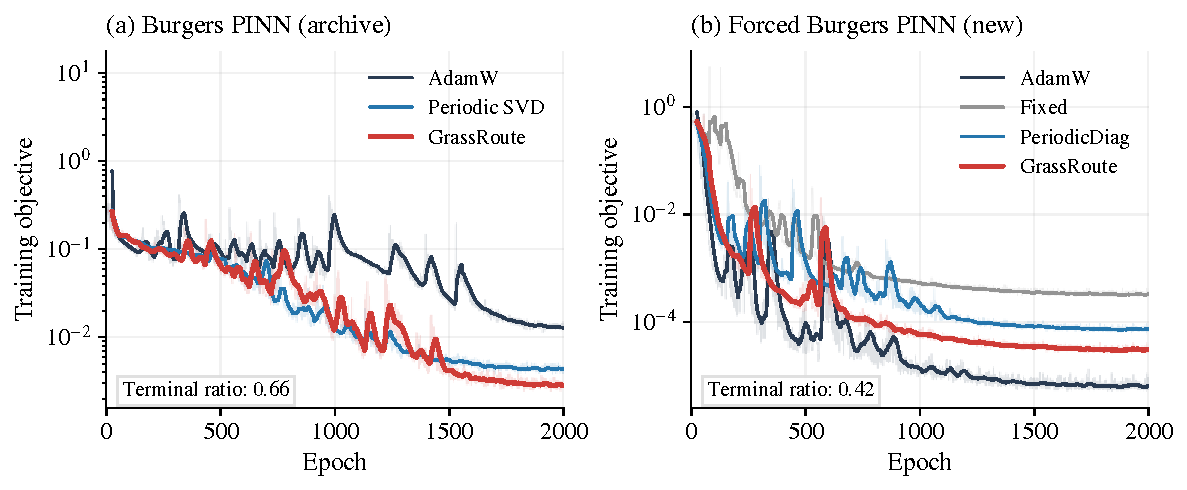
\includegraphics[width=\linewidth]{figures/fig_core_loss.pdf}
\caption{Core loss trajectories supporting the scientific-learning advantage,
with the competing outcomes retained. All panels show 2000 stored epochs:
faint lines are the raw objectives, solid lines are 25-epoch trailing means.
``Terminal ratio'' is the ratio of the final-100-epoch mean losses,
GrassRoute / periodic comparator; below one favors GrassRoute.
(a) Three archived Burgers trajectories: GrassRoute ends below AdamW and
periodic SVD. These stored curves are distinct from the tuned scalar summaries
in Table~\ref{tab:archive}; the objective is the archived residual-plus-initial-condition
loss, with its boundary-condition specification in Appendix~\ref{app:audit}.
(b) Independent validation-selected forced Burgers with corrected periodic
moment transport. GrassRoute improves on the matched-state periodic run;
AdamW remains stronger. The Poisson loss control appears in
Figure~\ref{fig:poisson-loss-control}. No best epoch is selected and no
cross-protocol loss magnitude is pooled. Seed 42 only.}
\label{fig:core-loss}
\end{figure*}
We distinguish archived results from a new validation-selected extension. They use different state-transport versions and, for several tasks, different data/model protocols. Their numerical endpoints are not pooled. All formal runs use seed 42, as specified by the proposal. The extension includes the official SubTrack++ optimizer; the historical B6 was an unofficial geodesic surrogate.

Figure~\ref{fig:core-loss} makes the positive loss evidence explicit rather
than inferring it from endpoint tables. The stored archived GrassRoute run
ends at $2.978\times10^{-3}$, compared with $1.368\times10^{-2}$ for AdamW
and $3.881\times10^{-3}$ for periodic SVD, with every intermediate epoch
retained. The independent follow-up panel shows where that advantage
transfers and where the strongest competing method remains better. Lower
training objective is not equated with lower held-out solution error.

\subsection{Scientific-learning and graph evidence}
The archived Burgers PINN supplies the clearest joint training-loss--state
observation: its tuned best loss is $1.97\times10^{-3}$ versus AdamW's
$1.10\times10^{-2}$ and periodic SVD's $3.27\times10^{-3}$, with 84.1\%
less persistent optimizer state. Figure~\ref{fig:core-loss} separately shows
all epochs of the stored trajectories. The archive reports a 1.78$\times$
step cost, and its residual-plus-initial-condition objective omits an explicit
spatial boundary penalty. This supports a scoped training-loss--memory result,
not a claim of superior physical solution accuracy. All recovered endpoints,
including the unsuccessful task families, remain in
Appendix~\ref{app:full-results}.

In the independent expanded-search Cora comparison, GrassRoute obtains
78.6\% test accuracy versus AdamW's 77.5\%, corrected periodic routing's
77.7\%, and official SubTrack++'s 77.3\%. Its persistent optimizer state is
207,368 bytes versus AdamW's 2,950,224, a 93.0\% reduction. SGD reaches
79.7\% with 1,475,100 bytes; thus GrassRoute supplies a favorable
accuracy--state operating point rather than the highest accuracy across
all six methods. The comparison uses the same nine-candidate validation budget
and fresh 1000-epoch formal runs (Table~\ref{tab:graph-strength}).

\input{figures/focused_gcn_main}
With the seed-42 Cora GraphSAGE hyperparameters frozen, three new initializations give mean final test accuracy 76.90\% for GrassRoute, 77.63\% for AdamW and 79.23\% for SGD-M. GrassRoute exceeds AdamW in 1/3 paired seeds. Corrected periodic SVD records 78.10\%, 78.60\% on its completed seeds and a retained numerical failure on the other. The favorable seed-42 accuracy--state observation is therefore not consistent across these new initializations; all endpoints and the failure appear in Table~\ref{tab:focused-cora-replication}.\par


\input{figures/revision_main_positive}

\subsection{Evaluation scope and complete reporting}
We distinguish strict primary-metric gains from accuracy--memory trade-offs.
The original proposal extension specified 27 representative configurations
and six methods, selected by validation before 1000 or 2000 complete formal
epochs. After 117 of 162 task--method runs finished, we stopped its remaining
high-cost image and continual-learning queue and redirected computation to
focused exploratory checks. This scope decision followed inspection of
completed results and cannot support a claim of prospective full coverage.
The original outcome matrix retains every completed, unfavorable and pending
cell in Appendix~\ref{app:full-results}. A controlled drifting-regression
study and a second Cora architecture are reported separately in
Appendix~\ref{app:focused-followup}. New public-data domains use another
frozen protocol below. All experiments use seed 42;
finite tuning budgets and one-seed observations do not imply statistical
significance or a universal optimizer ranking.

\subsection{Testing the mathematical mechanisms}
The controlled diagnostics isolate angle dependence at a fixed eigengap, QR/exponential discrepancy, and tracking under known population drift. They use full covariance spectra and actual oracle subspaces, with 600 random landscape checks and a 27-setting tracking bed. A separate neighboring-data experiment replaces one CIFAR-100 image while training a linear probe on frozen random ResNet features for 1000 epochs. It measures parameter and bounded-loss sensitivity, rather than equating a train--test gap with uniform stability. These auxiliary tests are not counted as additional end-to-end task-family wins. Their protocols and diagnostic tables appear in Appendix~\ref{app:audit}.

The complete mechanism grids, resource tables and expanded-search follow-ups are reported in Appendix~\ref{sec:strength-followup}.

\subsection{New public-data task domains}
\label{sec:new-public-tasks}
We add six tasks in three domains: raw-text classification (20 Newsgroups
and SMS Spam), structured-data classification (Adult and Spambase), and inverse
imaging (Optdigits denoising and missing-pixel completion)
\cite{sklearn20newsdata,uci2011sms,uci1996adult,uci1999spambase,uci1998optdigits}.
The two inverse tasks share the same image corpus and constitute two settings
within one domain, not two independent task-family replications. Dataset and
split definitions are fixed before formal training.

\begin{figure*}[htbp]\centering
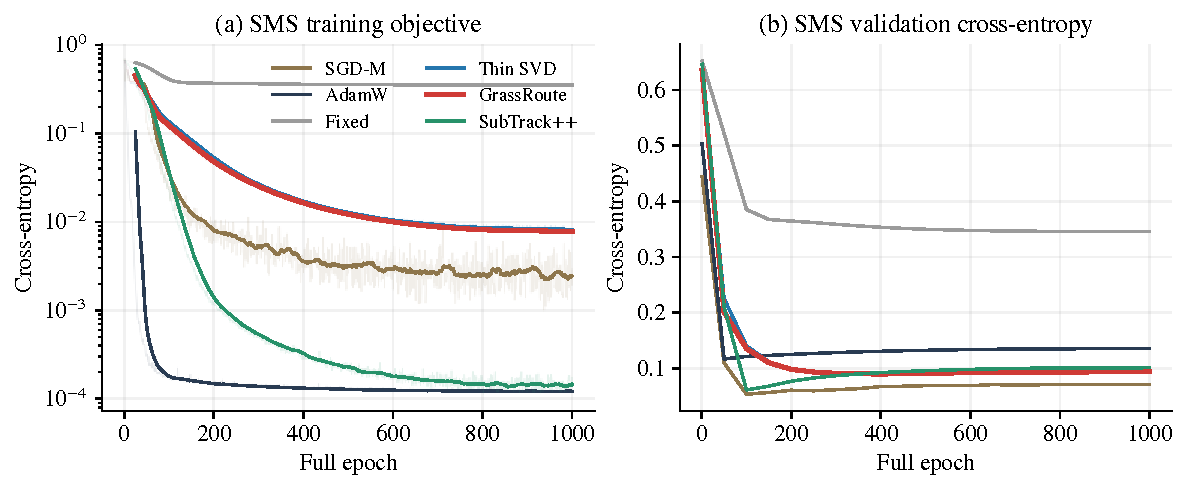
\includegraphics[width=\linewidth]{figures/fig_newtask_losses_selected.pdf}
\caption{SMS memory--quality operating point, with all six validation-selected methods. Left: the full 1000-epoch training objectives (raw losses faint, 25-epoch trailing means solid). Right: all saved validation cross-entropies. Hyperparameters were selected by final validation macro-F1; secondary cross-entropy did not replace that criterion. The full primary-metric matrix and every classifier endpoint remain in Tables~\ref{tab:newtasks-full} and~\ref{tab:newtasks-secondary}.}
\label{fig:newtasks-selected}
\end{figure*}


Every task compares SGD-M, AdamW, fixed routing, thin periodic SVD,
GrassRoute, and pinned official SubTrack++. All six receive nine 200-epoch
validation candidates and a fresh 1000-epoch selected run. Each epoch passes
through the complete training split in one full-data update. The routed grids
explicitly vary the residual/parallel learning-rate ratio across
$\{1,10,100\}$, since an SGD residual and an adaptive branch need not have
the same useful step-size scale. This changes the search protocol relative to
the original extension and is not silently pooled with it.

The periodic comparator directly factorizes the gradient matrix,
$G=L\Sigma V^\top$, and uses its top right singular vectors. This avoids
forming the full $G^\top G$ and transports both the first moment and the
diagonal second moment. Fixed and periodic methods store no unused routing
momentum. The complete search, sources and data hashes are frozen in the
new-task protocol; Appendix~\ref{app:new-task-full} reports every outcome.

The main-text subset uses an explicit reporting rule. A primary-metric gain
requires a better final held-out score than both AdamW and thin periodic SVD
after all six methods finish. A separate memory--quality trade-off requires
at least 50\% less state than AdamW, a primary classification score within
0.01 or an image MSE within 5\%, and a nondominated score--state point among
the six methods. The corresponding quality cost is stated explicitly. These are descriptive
one-seed criteria; statistical significance is not estimated.
The new public-data suite has completed 36 of 36 selected formal runs and 6 of six full comparisons. No completed new task currently establishes the predeclared gain over both AdamW and thin periodic SVD. Separate Pareto-efficient memory--quality trade-offs satisfy the predefined quality band on SMS / TF-IDF MLP. All attempted tasks and outcomes, including numerical failures and unfinished cells, remain in Appendix~\ref{app:new-task-full}; none is deleted after observing test results.

\par
% WWW table style: three rules, bold headers, reference green highlight.
\begin{table}[t]\centering\footnotesize
\caption{\textbf{SMS memory--quality trade-off.} Validation macro-F1 selects the configurations; test CE is secondary. The complete six-task comparison is in Table~\ref{tab:newtasks-full}. Persistent state is decimal MB.}
\label{tab:newtasks-selected}
\setlength{\tabcolsep}{5pt}
\reviewfit{\begin{tabular}{lrrr}\toprule {\bfseries Method} & {\bfseries F1 $\uparrow$} & {\bfseries Test CE $\downarrow$} & {\bfseries State MB $\downarrow$}\\\midrule
AdamW  &  95.48  &  0.1752  &  1.050\\
Thin SVD  &  94.29  &  0.0952  &  0.071\\
\rowcolor{oursbg}\textbf{GrassRoute} &  94.63  &  0.0931  &  0.137\\
\bottomrule\end{tabular}}\end{table}


On SMS, GrassRoute retains 0.137 MB versus AdamW's 1.050 MB (87.0\% less), with macro-F1 94.63 versus 95.48. Its separately retained test cross-entropy is 0.0931 versus 0.1752, and AUROC is 99.08 versus 98.28. These secondary probabilistic-quality observations did not determine the selected hyperparameters or redefine the primary F1 criterion. Every classifier endpoint is retained in Table~\ref{tab:newtasks-secondary}.

With the seed-42 validation choices frozen, the three new SMS initializations yield 94.74\% mean macro-F1 for GrassRoute, 95.48\% for AdamW and 94.29\% for thin periodic SVD. The GrassRoute state is 87.0\% smaller than AdamW's; its mean F1 is 0.74 points below AdamW. The one-point quality band holds in 1/3 seeds, and GrassRoute exceeds periodic SVD in 2/3 seeds. This is a descriptive mean memory--quality trade-off, with visible seed variability. All seeds and SGD appear in Table~\ref{tab:focused-sms-replication}.\par

\par

\section{Conclusion}
GrassRoute allocates adaptive state to an online Grassmann routing subspace
and preserves a full-dimensional residual update. Principal-plane geometry,
Householder identities and Ky Fan variational analysis yield sharp local
constants; a virtual iterate gives an averaged quadratic-root convergence
bound for the transported adaptive recursion. Full-state coupling and exact
Gaussian orientation costs connect the routing dynamics to conditional
stability and PAC-Bayes generalization, with Seeger--Maurer inversion and a
Haar-mixture prior retaining the geometry of learned directions.

The archived Burgers PINN, independent Cora comparison and new SMS task
identify favorable loss--state, accuracy--state and memory--quality operating
points under their specified protocols. Additional fixed-hyperparameter seeds
show that the Cora accuracy advantage is not consistent across initializations,
while the SMS average memory--quality trade-off varies by seed. The complete drift/noise grid
separates temporal averaging from tracking lag and state cost. Completed
endpoints, unfinished cells, the subsequent scope change and numerical-recovery
policies are recorded with the experimental protocols in the appendix.

\clearpage
\bibliographystyle{icml2026}
\bibliography{references}
\appendix
\onecolumn
% WWW table style: three rules, bold headers, reference green highlight.
\section{Detailed Theoretical Analysis}
\label{app:theory}

The proof is organized around three reductions: orthogonal routing to
independent principal planes; spectral perturbation to a separated Sylvester
equation; and generalization to an exact Gaussian KL followed by binary-KL
inversion. Their classical ingredients and their exact roles are explicit.
The parameter matrix is unconstrained, and a rank-$r$ optimizer state is not
a rank-$r$ parameter constraint. The table distinguishes sharp atomic
inequalities from the sufficient adaptive-state budgets used to combine them.

\begin{table}[htbp]
\centering\small
\caption{\textbf{Proof structure and sharpness.} Exactness concerns the stated
model or atomic inequality, not universal optimality of the complete optimizer
or of every composed finite-sample bound.}
\label{tab:proof-sharpness}
\setlength{\tabcolsep}{4pt}\renewcommand{\arraystretch}{1.18}
\reviewfit{\begin{tabular}{@{}p{.25\linewidth}p{.31\linewidth}p{.37\linewidth}@{}}
\toprule {\bfseries Reduction / classical tool} & {\bfseries Retained quantity} & {\bfseries Equality or scope}\\
\midrule
CS + Poincar\'e separation  &  QR pullback $L_R=\lambda_1-\lambda_d$  &  Two extremal eigenvectors; dimension-free and attained.\\
Ky Fan + square completion  &  Moving-excess coefficient $(1+a^{-1})/(4\Delta)$  &  Optimal to second order in a two-plane perturbation.\\
Principal-angle Rayleigh quotient  &  PL factor $2\Delta\cos^2R$  &  Rank one at angle $R$ attains it.\\
Householder involution  &  $\|D^2\mathcal C_\epsilon[E,E]\|_{\rm op}\le2\|E\|_F^2/\epsilon$  &  Attained at zero with rank-one $E$.\\
Davis--Kahan / Rosenblum  &  Off-diagonal residual divided by the mixed gap  &  Unit residual constant is exact for one Sylvester entry.\\
Descent + Minkowski  &  Quadratic-root stationarity  &  The reference quadratic attains the zero-defect noise coefficient.\\
Yule--Walker / Polyak  &  Exact modal stationary covariance  &  Additive tangent oracle; no multiplicative-noise identification.\\
Gaussian entropy identity  &  Exact prior--posterior angle cost  &  Identity for every positive two-variance covariance.\\
Seeger--Maurer  &  Exact $\Xi_n$ and binary-KL inverse  &  Bernoulli moment is exact; final confidence bound need not be optimal.\\
\bottomrule
\end{tabular}}
\end{table}
The actual Adam defect and the coupled state Lipschitz constants remain
sufficient upper bounds; sharpness is not claimed for those worst-case
budgets. A positive-gap tracking regime is also kept separate from a
stationarity limit in which that gap may vanish.

\subsection{Notation, filtration, and the population being tracked}
\label{app:population}

Write $\langle A,B\rangle=\operatorname{tr}(A^\top B)$ and let $\|\cdot\|$
denote the Frobenius norm unless the operator norm is explicitly indicated.
The pre-sampling filtration $\mathcal F_t$ contains the data set, parameters,
bases, and all optimizer states before drawing the current mini-batch.
Thus $W_t,U_t,M_{t-1},V_{t-1},H_{t-1}$ are measurable with respect to
$\mathcal F_t$. The sampled gradient $G_t$ generally is not. We use two
covariances:
\begin{align}
 S_t&=\mathbb E[G_t^\top G_t\mid\mathcal F_t],\label{eq:raw-cov}\\
 C_t&=\mathbb E\left[\frac{G_t^\top G_t}{\|G_t\|^2+\varepsilon_c}
                 \,\middle|\,\mathcal F_t\right].\label{eq:normalized-cov}
\end{align}
The implemented normalized tracker is unbiased for the tangent gradient of
$\Phi_t(U)=-\operatorname{tr}(U^\top C_tU)/2$. Its eigenspace is not in
general the leading eigenspace of $S_t$. Normalization preserves the eigenvectors
of a \emph{single} covariance sample; it need not preserve eigenvectors after
expectation. For example, let $G^\top G$ equal $100e_1e_1^\top$ with
probability $0.1$ and $e_2e_2^\top$ with probability $0.9$. With
$\varepsilon_c=0$, the unnormalized population selects $e_1$, whereas the
normalized population selects $e_2$. All tracking statements refer to $C_t$;
raw residual-energy statements refer to $S_t$. They coincide up to scale only
under an additional structural assumption, such as deterministic gradient norm.

For a fixed covariance $C\succeq0$, put
\begin{equation}
 \lambda_1\ge\cdots\ge\lambda_d,\quad
 \Delta=\lambda_r-\lambda_{r+1}>0,\quad
 \Lambda=\lambda_1-\lambda_d,\quad
 P=UU^\top,\quad P_\star=U_\star U_\star^\top.
\end{equation}
Here $U_\star$ spans the leading eigenspace. Let
$\theta_1,\ldots,\theta_r\in[0,\pi/2]$ be the principal angles and define
\begin{equation}
 R(U)=\|\Theta\|_F,\quad \theta_{\max}(U)=\max_i\theta_i,
 \quad s(U)=\|\sin\Theta\|_F,\quad h_C(U)=\Phi(U)-\Phi(U_\star).
\end{equation}
The angle $\theta_{\max}$ controls transversality to the optimal subspace;
$R$ is geodesic distance. They must not be identified with the distance between
two consecutive optimizer bases. Constants in the analysis are specific to a
layer, rank, and time interval. A positive average captured energy across layers
does not verify a uniform lower bound on their individual eigengaps.

\subsection{Quotient geometry and implemented operations}

The canonical quotient metric on $\mathrm{Gr}(r,d)$ has horizontal lift
\begin{equation}
 \mathcal H_U=\{\xi:U^\top\xi=0\},\qquad
 \Pi_U(A)=(I-P)A,\qquad g_U(\xi,\zeta)=\langle\xi,\zeta\rangle.
\end{equation}
Equivalently, for projector tangent vectors the metric is half the ambient
Frobenius inner product. These normalizations agree under
$\dot P=\xi U^\top+U\xi^\top$ \cite{bendokat2024grassmann}.
This metric has nonnegative sectional curvature bounded by $2$; the upper
bound need not be attained in every low-dimensional case
\cite{zimmermann2024curvature}. The injectivity radius is $\pi/2$.
The cut locus relative to $[U_\star]$ consists of subspaces having at least
one principal angle $\pi/2$. Consequently $\theta_{\max}<\pi/2$ ensures
the usual graph chart exists, while $R<\pi/2$ is a sufficient, stronger
condition. Neither condition implies geodesic convexity of $\Phi$ throughout
that region.

\begin{lemma}[Projection and exact energy accounting]
\label{lem:decomposition}
For every $G$ and orthonormal $U$,
\begin{equation}
 G=GP+G(I-P),\qquad
 \|G\|^2=\|GU\|^2+\|G(I-P)\|^2.
\end{equation}
For a covariance $S=\mathbb E[G^\top G]$, an
$\mathcal F_t$-measurable projector satisfies
\begin{equation}
 \mathbb E_t\|G(I-P)\|^2
 =\operatorname{tr}(S)-\operatorname{tr}(U^\top SU)
 =\tau_r(S)+2h_S(U),\label{eq:tail-exact}
\end{equation}
where $\tau_r(S)=\sum_{j>r}\lambda_j(S)$.
\end{lemma}
\begin{proof}
The two gradient components are orthogonal because $P(I-P)=0$. Also
$\|GP\|^2=\operatorname{tr}(U^\top G^\top GU)=\|GU\|^2$.
Taking conditional expectation yields the first equality in
\eqref{eq:tail-exact}; adding and subtracting the leading $r$ eigenvalues
yields the second. If $P$ is chosen from the \emph{current} sampled gradient,
the conditional-expectation step requires separate justification.
\end{proof}

\begin{lemma}[QR retraction and its quotient error]
\label{lem:qr}
Let $\xi\in\mathcal H_U$ have compact singular value decomposition
$\xi=A\operatorname{diag}(\sigma_i)B^\top$. The projector of
$\mathrm{qf}(U+\xi)$ is
\begin{equation}
 P_{\mathrm{QR}}=(U+\xi)(I+\xi^\top\xi)^{-1}(U+\xi)^\top.
 \label{eq:qr-projector}
\end{equation}
In the principal planes of $\xi$, QR and the exponential map rotate through
$\arctan\sigma_i$ and $\sigma_i$, respectively. If $\|\xi\|\le1/4$,
\begin{equation}
 d_{\mathrm{Gr}}([\mathrm{qf}(U+\xi)],\operatorname{Exp}_{[U]}\xi)
 \le\frac13\Big(\sum_i\sigma_i^6\Big)^{1/2}
 \le\frac13\|\xi\|^3.\label{eq:qr-exp}
\end{equation}
Projection transport $\mathcal T_{U\to V}\xi=(I-VV^\top)\xi$ is
nonexpansive and satisfies
\begin{equation}
 \|\mathcal T_{U\to V}\xi-\xi\|
 \le\|VV^\top-UU^\top\|_{\mathrm{op}}\|\xi\|.
\end{equation}
\end{lemma}
\begin{proof}
Horizontal tangency gives $(U+\xi)^\top(U+\xi)=I+\xi^\top\xi$,
which is positive definite for every $\xi$. The orthogonal projector onto its
column span is therefore \eqref{eq:qr-projector}. The polar representative
$(U+\xi)(I+\xi^\top\xi)^{-1/2}$ has exactly the same span as its QR
representative. In the $i$th principal plane its coefficients are
$(1,\sigma_i)/\sqrt{1+\sigma_i^2}$, giving angle
$\arctan\sigma_i$. The exponential coefficients are
$(\cos\sigma_i,\sin\sigma_i)$. The small-step condition prevents angle
wrapping. Since
$0\le x-\arctan x=\int_0^x t^2/(1+t^2)\,dt\le x^3/3$,
summing squared angular differences proves \eqref{eq:qr-exp}.
Finally, orthogonal projection cannot increase norm and
$(I-VV^\top)\xi-\xi=(UU^\top-VV^\top)\xi$.
\end{proof}

This calculation identifies the retraction error on the quotient, where the
algorithm actually tracks a subspace. The QR basis itself can also contain a
within-subspace rotation. That rotation affects coordinatewise Adam even when
it has no effect on the routing objective. Numerical orthogonality error,
retraction approximation error, and statistical tracking error are three
different quantities; a small value of the first does not establish either of
the others.

\subsection{The routing landscape: exact principal-angle analysis}
\label{app:landscape}

\begin{theorem}[Landscape, local PL inequality, and its boundary]
\label{thm:landscape}
For $C\succeq0$ with gap $\Delta>0$, the unique minimizing subspace of
$\Phi(U)=-\operatorname{tr}(U^\top CU)/2$ is $[U_\star]$.
Its horizontal gradient and Hessian quadratic form are
\begin{align}
 \operatorname{grad}\Phi(U)&=-(I-P)CU,\label{eq:grass-grad}\\
 \langle\xi,\operatorname{Hess}\Phi(U)[\xi]\rangle
 &=\operatorname{tr}(\xi^\top\xi\,U^\top CU)
   -\operatorname{tr}(\xi^\top C\xi).\label{eq:grass-hess}
\end{align}
Globally,
\begin{equation}
 \frac\Delta2s(U)^2\le h_C(U)\le\frac\Lambda2s(U)^2,
 \qquad \frac2\pi R(U)\le s(U)\le R(U).\label{eq:gap-bounds}
\end{equation}
Whenever $\theta_{\max}(U)\le R_0<\pi/2$,
\begin{equation}
 \|\operatorname{grad}\Phi(U)\|^2
 \ge2\Delta\cos^2 R_0\,h_C(U).\label{eq:PL}
\end{equation}
At the minimum the Hessian eigenvalues are
$\lambda_i-\lambda_j$, $i\le r<j$. Every nonoptimal critical subspace
has a tangent direction of curvature at most $-\Delta$.
Quadratic growth in \eqref{eq:gap-bounds} and PL in \eqref{eq:PL} do
\emph{not} assert geodesic strong convexity on the entire normal neighborhood.
\end{theorem}

\begin{proof}
The variational characterization of eigenvalues gives
$\max_{U^\top U=I}\operatorname{tr}(U^\top CU)=\sum_{i\le r}\lambda_i$.
The gap separates this maximizing subspace from its complement, giving
uniqueness on the quotient. Differentiating $\Phi$ in the ambient space gives
$-CU$; horizontal projection proves \eqref{eq:grass-grad}.
For a Grassmann geodesic with $\dot U(0)=\xi$, one can choose a horizontal
lift satisfying $\ddot U(0)=-U\xi^\top\xi$. Differentiating
$-\operatorname{tr}(U(t)^\top CU(t))/2$ twice proves
\eqref{eq:grass-hess}.

Choose principal vectors $x_i\in[U_\star]$ and
$y_i\in[U_\star]^\perp$ so the columns of a representative of $U$ are
\begin{equation}
 u_i=x_i\cos\theta_i+y_i\sin\theta_i.
\end{equation}
Terms with $\theta_i=0$ need no complementary vector; when the complement
has dimension smaller than $r$, only the nonzero-angle pairs are used.
The $x_i$ form an orthonormal basis for $[U_\star]$ and the relevant
$y_i$ are orthonormal. Since this leading subspace is invariant under $C$,
$x_i^\top Cy_j=0$. Put $a_i=x_i^\top Cx_i$,
$b_i=y_i^\top Cy_i$, and $c_i=a_i-b_i$. Then
\begin{equation}
 h_C(U)=\frac12\sum_i c_i\sin^2\theta_i,
 \qquad \Delta\le c_i\le\Lambda.\label{eq:CS-excess}
\end{equation}
This is an exact excess formula in principal coordinates. The coefficients
$c_i$ are Rayleigh quotients, not generally individual eigenvalue
differences. The bounds on $c_i$ prove the first part of
\eqref{eq:gap-bounds}; $2x/\pi\le\sin x\le x$ on $[0,\pi/2]$
proves the second.

For every nonzero angle set
$e_i=-x_i\sin\theta_i+y_i\cos\theta_i$. The matrix tangent directions
which place $e_i$ in column $i$ and zero elsewhere are orthonormal and
horizontal. Direct differentiation gives their gradient components
$c_i\sin\theta_i\cos\theta_i$. Bessel's inequality therefore gives
\begin{align}
 \|\operatorname{grad}\Phi(U)\|^2
 &\ge\sum_i c_i^2\sin^2\theta_i\cos^2\theta_i\\
 &\ge\Delta\cos^2R_0\sum_i c_i\sin^2\theta_i
 =2\Delta\cos^2R_0\,h_C(U).
\end{align}
This proves PL without a curvature-comparison shortcut. It is consistent
with prior analyses of the block Rayleigh quotient
\cite{alimisis2024geodesic}; the angular factor is not claimed as a new
standalone manifold theorem.

At $U_\star$, diagonalize $C$ in its invariant subspaces. A tangent
coordinate moving selected eigenvector $i$ toward unselected eigenvector
$j$ has Hessian eigenvalue $\lambda_i-\lambda_j$. For a critical point,
$(I-P)CU=0$, so its selected subspace is invariant. If it is not leading,
some selected eigenvector has eigenvalue at most $\lambda_{r+1}$ and some
unselected one has eigenvalue at least $\lambda_r$. Rotating the former
toward the latter gives Hessian curvature at most $-\Delta$.
Finally, for $r=1,d=2$,
\begin{equation}
 h(\theta)=\frac\Delta2\sin^2\theta,\qquad
 h''(\theta)=\Delta\cos(2\theta).
 \label{eq:nonconvex-counterexample}
\end{equation}
Thus the Hessian is negative for $\pi/4<\theta<\pi/2$ even though
quadratic growth and the positive PL bound still hold.
\end{proof}

The distinction in the last sentence is essential for tracking and stability.
PL controls objective decrease along one trajectory. Contraction of the
distance between \emph{two} trajectories requires additional hypotheses;
it does not follow from PL alone. Nor does \eqref{eq:PL} prove that the
scalar $\Delta\cos^2R_0$ predicts the ranking of complete neural-network
optimizers. Gradient noise, covariance normalization, parameter-state
conditioning, and computational cost remain independent factors.

\subsection{Coordinate transport and the limits of diagonal Adam}
\label{app:transport}

\begin{lemma}[First moments and diagonal second moments]
\label{lem:moments}
Let $U_+=UQ$ for $Q\in O(r)$, representing a pure basis change. Then
$Z_+=ZQ$ and exact first-moment consistency requires $M_+=MQ$.
For a row-wise full second moment $B_i=\mathbb E[z_i^\top z_i]$,
the exact transformation is $B_{i,+}=Q^\top B_iQ$. If only its diagonal
$v_i$ is stored, the diagonal-covariance approximation is
\begin{equation}
 v_{i,+}=v_i Q^{\odot2},\label{eq:diag-transport}
\end{equation}
and its error is precisely
\begin{equation}
 \operatorname{diag}(Q^\top B_iQ)-v_iQ^{\odot2}
 =\operatorname{diag}\{Q^\top(B_i-\operatorname{Diag}v_i)Q\}.
 \label{eq:offdiag-error}
\end{equation}
The error need not be second order in the basis rotation. Furthermore,
coordinatewise Adam is not invariant under general $Q$, even with an
exactly transformed diagonal.
\end{lemma}
\begin{proof}
$G(UQ)=(GU)Q$ gives the first claim and
$(MQ)(UQ)^\top=MU^\top$ verifies the lifted first moment.
For second moments, expand $(z_iQ)^\top(z_iQ)$ and take expectation.
Its diagonal under the approximation $B_i=\operatorname{Diag}v_i$ is
$\sum_k v_{ik}Q_{kj}^2$, proving \eqref{eq:diag-transport} and
\eqref{eq:offdiag-error}. For $Q=I+\epsilon A+O(\epsilon^2)$,
the omitted off-diagonal covariance can contribute a linear term through
$\operatorname{diag}(B_iA-AB_i)$.
Finally, entrywise division by a diagonal square root does not commute with
orthogonal mixing. For example, the zero-history, negligible-$\varepsilon$
Adam direction for $z=(2,1)$ is $(1,1)$. A generic rotation followed by
coordinatewise normalization and rotation back does not reproduce that
vector. Signed coordinate permutations are a special invariant case.
\end{proof}

For consecutive, genuinely different subspaces we use
$R=\operatorname{Polar}(U_+^\top U)$ and align $M_+=MR^\top$.
This minimizes basis mismatch, but cannot restore the part of a historical
ambient moment orthogonal to the new span. If an ambient moment is $A$,
then
\begin{equation}
 \|AP-AP_+\|\le\|A\|\|P-P_+\|_{\mathrm{op}}
 =\|A\|\sin\theta_{\max}(U,U_+).
\end{equation}
This is a first-order perturbation bound, not an exact transport identity.
The covariance error from omitted correlations must be added separately.

The archived implementation used $(\sqrt v\,Q)^{\odot2}$ rather than
\eqref{eq:diag-transport}. These differ even for diagonal covariance:
with $v=(1,1)$ and a $45$-degree rotation the former gives $(2,0)$ up to
column order, while the correct diagonal is $(1,1)$. New experiments use
\eqref{eq:diag-transport}; historical outcomes retain their original
algorithm label. Resetting $v$ to zero is another distinct algorithm. A
reset is a deterministic state transformation, not a generic additive
statistical error, and its effect on descent must be analyzed through the
resulting parameter direction.

\subsection{Stochastic online tracking with an explicit perturbation budget}
\label{app:tracking}

The landscape result concerns a fixed covariance. During training both its
eigenvectors and eigenvalues change, and the tracked basis is driven by noisy
mini-batches. We first establish a finite-horizon bound on objective excess.
This avoids silently replacing PL by a two-trajectory contraction property.

\begin{assumption}[Bounded, separated tracking interval]
\label{ass:tracking}
On the interval considered, $C_t\succeq0$,
$\|C_t\|_{\mathrm{op}}\le C_0$, and
$\lambda_r(C_t)-\lambda_{r+1}(C_t)\ge\Delta_0>0$.
Every update remains in the region
$\theta_{\max}(U_t,U_t^\star)\le R_0<\pi/2$.
Its descent representation is
\begin{equation}
 U_{t+1}=\operatorname{Retr}_{U_t}\{-\rho_t(g_t+\zeta_t+b_t)\},
 \qquad g_t=\operatorname{grad}\Phi_t(U_t),\label{eq:tracking-update}
\end{equation}
where $\mathbb E_t\zeta_t=0$,
$\mathbb E_t\|\zeta_t\|^2\le\sigma_t^2$, and
$\mathbb E_t\|b_t\|^2\le B_t^2$.
The retraction pullback satisfies
\begin{equation}
 \Phi_t(\operatorname{Retr}_U\xi)
 \le\Phi_t(U)+\langle\operatorname{grad}\Phi_t(U),\xi\rangle
                    +\frac{L_R}{2}\|\xi\|^2\label{eq:pullback-smooth}
\end{equation}
for all actual steps, and
$\|C_{t+1}-C_t\|\le v_t$ almost surely, with deterministic $v_t$.
\end{assumption}

Proposition~\ref{prop:qr-calculus} verifies \eqref{eq:pullback-smooth}
with the sharp, dimension-free choice
$L_R=\sup_t[\lambda_1(C_t)-\lambda_d(C_t)]\le C_0$.
No small-angle assumption is required for this pullback inequality itself;
the principal-angle restriction is used only by the PL inequality.

The bias $b_t$ records deviations from a fresh stochastic tangent-gradient
step. It includes the Grassmann momentum lag, deterministic approximation
errors, and any clipping bias. It is permitted to correlate with $\zeta_t$.
This is useful for the implemented momentum, whose error cannot be treated
as independent zero-mean noise.

\begin{lemma}[Ky Fan completion of squares for moving objective excess]
\label{lem:excess-drift}
Let $C,C'$ be symmetric, let $C$ have rank-$r$ gap at least $\Delta_0>0$,
and put $v=\|C'-C\|_F$. No gap assumption on $C'$ is needed. For every
rank-$r$ projector $P$ and every $a>0$,
\begin{equation}
 h_{C'}(P)\le(1+a)h_C(P)+\frac{1+a^{-1}}{4\Delta_0}v^2.
 \label{eq:excess-drift}
\end{equation}
For fixed $a$, the coefficient $(1+a^{-1})/4$ is optimal to second order.
\end{lemma}
\begin{proof}
Let $P_\star,P_\star'$ maximize the respective Ky Fan traces
\cite{fan1951maximum}, $E=C'-C$, and $D=P_\star'-P_\star$. Then
\begin{align}
 h_{C'}(P)-h_C(P)
 &=\tfrac12\operatorname{tr}\{E(P_\star-P)\}
                      +\tfrac12\operatorname{tr}(C'D),\\
 \tfrac12\operatorname{tr}(C'D)
 &=-h_C(P_\star')+\tfrac12\langle E,D\rangle\\
 &\le-\tfrac14\Delta_0\|D\|_F^2+\tfrac12v\|D\|_F
 \le\frac{v^2}{4\Delta_0}.
\end{align}
The last line completes a square, retaining the curvature term which a
plain perturbation-norm estimate discards. Also,
\begin{equation}
 \tfrac12|\langle E,P_\star-P\rangle|
 \le v\sqrt{h_C(P)/\Delta_0}
 \le a h_C(P)+\frac{v^2}{4a\Delta_0}.
\end{equation}
For sharpness take $r=1,d=2$,
$C=\gamma I+\operatorname{Diag}(\Delta_0,0)$, $\gamma>0$,
$E_e=\left(\begin{smallmatrix}0&e\\e&0\end{smallmatrix}\right)$,
and $P_e=u_eu_e^\top$ with $u_e=(\cos\theta_e,\sin\theta_e)$,
$\theta_e=-e/(a\Delta_0)$. Direct diagonalization gives
\begin{equation}
 \lim_{e\to0}\frac{\Delta_0\{h_{C+E_e}(P_e)-(1+a)h_C(P_e)\}}
                         {\|E_e\|_F^2}=\frac{1+a^{-1}}4.
\end{equation}
\end{proof}

\begin{theorem}[Tracking with unrounded contraction and perturbation constants]
\label{thm:tracking}
Under Assumption~\ref{ass:tracking}, let
$\mu=\Delta_0\cos^2R_0$, $\alpha_t=\rho_t\mu$,
$L_R\rho_t\le1/4$, and $\alpha_t\le1/2$. Define
\begin{align}
 q_t&=(1+\alpha_t/2)(1-\alpha_t),\\
 A_t&=2(1+\alpha_t/2)
                 (L_R\rho_t^2\sigma_t^2+\rho_tB_t^2)
                  +\left(\frac1{2\alpha_t}+\frac14\right)
                                      \frac{v_t^2}{\Delta_0}.
\end{align}
For $h_t=h_{C_t}(U_t)$,
\begin{align}
 \mathbb E h_{t+1}&\le q_t\mathbb E h_t+A_t,
 \label{eq:tracking-recursion}\\
 \mathbb E h_T&\le h_0\prod_{j<T}q_j+
                  \sum_{t<T}A_t\prod_{j=t+1}^{T-1}q_j.
 \label{eq:tracking-unrolled}
\end{align}
For constant bounds and step $\rho$, with
$\alpha=\rho\mu$ and $\chi_\alpha=(1+\alpha/2)/(1+\alpha)$,
\begin{equation}
 \limsup_T\mathbb E h_T\le\chi_\alpha\left[
       \frac{4L_R\rho\sigma^2}{\mu}+\frac{4B^2}{\mu}
                      +\frac{v^2}{\rho^2\mu^2\Delta_0}\right].
 \label{eq:tracking-floor}
\end{equation}
Moreover $\mathbb E d_{\rm Gr}(U_T,U_T^\star)^2
\le\pi^2\mathbb Eh_T/(2\Delta_0)$.
\end{theorem}
\begin{proof}
For $h_t^+=h_{C_t}(U_{t+1})$, sharp QR pullback smoothness,
$\mathbb E_t\zeta_t=0$, and Young's inequality give
\begin{align}
 \mathbb E_t h_t^+
 &\le h_t-\rho_t\|g_t\|^2
       -\rho_t\langle g_t,\mathbb E_tb_t\rangle
       +\tfrac12L_R\rho_t^2\mathbb E_t\|g_t+\zeta_t+b_t\|^2\\
 &\le h_t-\tfrac12\rho_t\|g_t\|^2
                          +2L_R\rho_t^2\sigma_t^2+2\rho_tB_t^2\\
 &\le(1-\alpha_t)h_t+2L_R\rho_t^2\sigma_t^2+2\rho_tB_t^2.
 \label{eq:frozen-tracking}
\end{align}
Here $\rho_t|\langle g_t,\mathbb E_tb_t\rangle|
\le\rho_t\|g_t\|^2/4+\rho_tB_t^2$ and
$\mathbb E_t\|g_t+\zeta_t+b_t\|^2
\le2\|g_t\|^2+4\sigma_t^2+4B_t^2$; the step condition gives the
second line. Apply Lemma~\ref{lem:excess-drift} pathwise at $U_{t+1}$
with $a=\alpha_t/2$ and keep its constants to obtain the stated recursion.
Unroll it and use $1-q=\alpha(1+\alpha)/2$ for the steady bound.
The angle bound follows from quadratic growth and
$\sin\theta\ge2\theta/\pi$. Only the atomic smoothness and excess-drift
constants are claimed sharp; the stochastic bias budget is sufficient.
\end{proof}

The noise term increases with $\rho$, whereas the drift term decreases
with $\rho^2$. For the noise-and-drift terms, dropping
$\chi_\alpha\le1$ gives the envelope $A\rho+D/\rho^2$, whose minimizer is $\rho=(2D/A)^{1/3}$, subject to the
admissible-step restrictions. This is an explicit tracking trade-off, not a
claim that larger drift always increases GrassRoute's advantage over SVD.
If covariance changes are driven by the parameter update and
$\|C(W')-C(W)\|\le L_C\|W'-W\|$, then
\begin{equation}
 v_t\le L_C\eta_t\|D_t\|.
 \label{eq:coupling-drift}
\end{equation}
With bounded directions, a sufficient scaling for the drift contribution
in \eqref{eq:tracking-floor} to be $O(T^{-1/2})$ is
$\rho=O(T^{-1/2})$ and $v=O(T^{-3/4})$. The weaker assertion
$v=o(T^{-1/2})$ only implies a vanishing drift floor, without that rate.
Different schedules can trade parameter speed for tracking accuracy.

\paragraph{Momentum and retraction have separate costs.}
For the implemented update,
$H_t=\mu_H\Pi_{U_t}H_{t-1}+(1-\mu_H)\widehat Q_t$.
Writing $\widehat Q_t=Q_t+\epsilon_t$ and subtracting $Q_t$ gives
\begin{equation}
 H_t-Q_t=\mu_H\Pi_{U_t}(H_{t-1}-Q_{t-1})
 +\mu_H(\Pi_{U_t}Q_{t-1}-Q_t)+(1-\mu_H)\epsilon_t.
 \label{eq:momentum-lag}
\end{equation}
Minkowski's inequality and nonexpansiveness imply an $L_2$ lag bound
$e_t\le\mu_He_{t-1}+\mu_HD_t+(1-\mu_H)\sigma_t$, where
$D_t$ bounds the transported population-direction change. In a stationary
region with $D_t\le D$, this gives
$\limsup e_t\le\mu_HD/(1-\mu_H)+\sigma$.
The familiar variance reduction factor $(1-\mu_H)/(1+\mu_H)$ holds for
an EMA of independent noise at a \emph{frozen} basis; it cannot be assumed
for moving, data-dependent bases. Equation~\eqref{eq:momentum-lag}
states exactly which additional terms must be controlled.

If QR is compared with an exponential step of the \emph{same} tangent
direction, Lemma~\ref{lem:qr} gives a local $O(\rho_t^3\|H_t\|^3)$
subspace difference. When QR is analyzed directly through
\eqref{eq:pullback-smooth}, that error is already accounted for in the
pullback constant; adding it again as independent noise would double count.
Neither the curvature upper bound nor positive curvature alone supplies a
universal signed correction to the tracking recursion.

\paragraph{Continuous motion and jumps.}
Davis--Kahan also gives
$s(U_{t+1}^\star,U_t^\star)\le\sqrt2v_t/\Delta_0$.
A small covariance increment therefore bounds target motion. The converse
does not hold, since eigenvalues can change without rotating the target.
Theorem~\ref{thm:tracking} uses $v_t$ as a conservative observable control.
An abrupt change that violates the angle neighborhood invalidates the local
guarantee; it need not cause divergence, and no deterministic ordering
between online tracking and periodic recomputation follows. Boundary
experiments should test the effect of jump size while holding the spectrum
and gradient noise fixed.

\subsection{Explicit differential calculus, graph coordinates, and discrete contraction}
\label{app:formal-geometry}
Throughout this subsection $C=C^\top$, $\Delta>0$, and $\|\cdot\|=\|\cdot\|_F$.

\begin{proposition}[Two-plane QR calculus; sharp pullback constant]
\label{prop:qr-calculus}
Let $C=C^\top$, $\Lambda_C=\lambda_1(C)-\lambda_d(C)$, and $U^\top\xi=0$.
For $P=UU^\top$,
\begin{align}
 T_P\mathrm{Gr}&=\{J=J^\top:PJ+JP=J\},\\
 J&=\xi U^\top+U\xi^\top,&\|J\|_F^2&=2\|\xi\|_F^2,\\
 \mathcal P_P(A)&=[P,[P,A]],&\dot P&=[P,[P,C]].
 \label{eq:double-bracket}
\end{align}
The QR pullback $F_U(s)=\Phi(\mathrm{qf}(U+s\xi))$ obeys, for all real $s$,
\begin{align}
 |F_U''(s)|&\le\Lambda_C\|\xi\|_F^2,\\
 \Phi(\mathrm{qf}(U+\xi))
 &\le\Phi(U)+\langle\operatorname{grad}\Phi(U),\xi\rangle
                                  +\tfrac12\Lambda_C\|\xi\|_F^2.
 \label{eq:explicit-pullback}
\end{align}
The constant $\Lambda_C$ is optimal uniformly over $U,\xi$.
\end{proposition}
\begin{proof}
The projector identities follow from $D(P^2-P)[J]=PJ+JP-J$.
For the quantitative bound use the singular-vector/CS decomposition
\citep[Chapters 2 and 8]{golub2013matrix}. After a right orthogonal change,
write $\xi_i=\sigma_iv_i$, with $(u_i,v_i)$ orthonormal for each
$\sigma_i>0$. Its QR span has the orthonormal polar representative
\begin{equation}
 q_i(s)=\frac{u_i+s\sigma_iv_i}{\sqrt{1+s^2\sigma_i^2}}.
\end{equation}
Zero singular values contribute constant columns.
Put $a_i=u_i^\top Cu_i$, $b_i=u_i^\top Cv_i$, $c_i=v_i^\top Cv_i$.
Poincar\'e separation for the $2\times2$ compression of $C$ gives
\begin{equation}
 \sqrt{(a_i-c_i)^2+4b_i^2}\le\Lambda_C.
\end{equation}
The trace is a sum of scalar Rayleigh quotients:
\begin{align}
 F_U(s)&=-\frac12\sum_i
       \frac{a_i+2s\sigma_ib_i+s^2\sigma_i^2c_i}{1+s^2\sigma_i^2},\\
 F_{U,i}''(s)&=\sigma_i^2
 \frac{(a_i-c_i)(1-3z_i^2)+2b_i z_i(3-z_i^2)}{(1+z_i^2)^3},
 \qquad z_i=s\sigma_i.
\end{align}
The cancellation
\begin{equation}
 (1-3z^2)^2+z^2(3-z^2)^2=(1+z^2)^3
\end{equation}
yields $|F_{U,i}''(s)|\le
\Lambda_C\sigma_i^2/(1+z_i^2)^{3/2}\le\Lambda_C\sigma_i^2$.
Sum and integrate the second derivative. At $s=0$, take $r=1$,
$u$ a lowest eigenvector and $\xi$ a unit highest eigenvector;
$F_U''(0)=-\Lambda_C$. Interchanging them gives $+\Lambda_C$.
Thus both the absolute and upper pullback constants are attained.
\end{proof}

\begin{lemma}[Stored QR frames and aligned moment transport]
\label{lem:qr-frame}
Let $U^\top\xi=0$, let $Q(s)R(s)=U+s\xi$ be the thin QR decomposition
with positive diagonal in $R(s)$, and put $U_+=Q(1)$,
$O=\operatorname{Polar}(U_+^\top U)$. Then
\begin{align}
 \sigma_{\min}(U+s\xi)&\ge1, &\|U_+-U\|&\le\sqrt3\|\xi\|,\\
 \|O-I\|&\le2\sqrt3\|\xi\|, &
 \|U_+O-U\|_{\rm op}&=2\sin(\theta_{\max}/2)
                      \le d_{\rm Gr}(U_+,U)\le\|\xi\|.\label{eq:frame-bounds}
\end{align}
The row-vector transport $\mathcal T(XU^\top)=XO^\top U_+^\top$ is an
isometry on the old routed space and satisfies
\begin{equation}
 \|\mathcal T(XU^\top)-XU^\top\|\le\|X\|\,\|\xi\|.\label{eq:transport-near-identity}
\end{equation}
On a segment of full-rank matrices with $\sigma_{\min}\ge s_0>0$,
\begin{equation}
 \|\mathrm{qf}(A)-\mathrm{qf}(B)\|
       \le\frac{\sqrt3}{s_0}\|A-B\|.\label{eq:qr-explicit-lip}
\end{equation}
\end{lemma}
\begin{proof}
Differentiate $A=QR$ and set $K=Q^\top\dot A R^{-1}$:
\begin{align}
 \dot Q&=(I-QQ^\top)\dot A R^{-1}+Q\Omega,\\
 \Omega&=Q^\top\dot Q=-\Omega^\top,\qquad
 \operatorname{strictlower}(\Omega)=\operatorname{strictlower}(K),\\
 \|\Omega\|^2&=2\|\operatorname{strictlower}(K)\|^2\le2\|K\|^2,\\
 \|\dot Q\|^2
 &\le3\|\dot A R^{-1}\|^2
 \le\frac{3\|\dot A\|^2}{\sigma_{\min}(A)^2}.
\end{align}
Integrate along $U+s\xi$ or the stipulated segment. For $B=U_+^\top U$,
\begin{equation}
 \|\operatorname{Polar}(B)-I\|
 \le\frac{2\|B-I\|}{\sigma_{\min}(B)+1}
 \le2\|U_+-U\|.
\end{equation}
This polar perturbation inequality follows from the Sylvester equation for
the polar differential, or its integrated two-point form. Singular-value
decomposition of $U_+^\top U$ gives the aligned-frame singular values
$2\sin(\theta_i/2)$; Lemma~\ref{lem:qr} gives
$\theta_i=\arctan\sigma_i(\xi)$. Isometry and
\eqref{eq:transport-near-identity} follow by right multiplication.
\end{proof}

\begin{proposition}[An exact graph flow and contraction of the implemented QR step]
\label{prop:graph-flow}
Let $E=(E_1,E_2)$ diagonalize $C$, with blocks
$\Lambda_1=\operatorname{Diag}(\lambda_1,\ldots,\lambda_r)$ and
$\Lambda_2=\operatorname{Diag}(\lambda_{r+1},\ldots,\lambda_d)$.
For $K\in\mathbb R^{(d-r)\times r}$ define
\begin{align}
 S_K&=I+K^\top K,&B_K&=S_K^{-1/2},\\
 U(K)&=(E_1+E_2K)B_K,&P(K)&=U(K)U(K)^\top.
\end{align}
Then
\begin{align}
 \tan\theta_i&=\sigma_i(K),&
 h_C(K)&=\tfrac12\operatorname{tr}
  \big[(\Lambda_1K^\top K-K^\top\Lambda_2K)S_K^{-1}\big].\label{eq:graph-excess}
\end{align}
The exact continuous Grassmann ascent flow and its solution are
\begin{align}
 \dot K&=\Lambda_2K-K\Lambda_1=:\mathcal L K,\\
 K(t)&=e^{t\Lambda_2}K(0)e^{-t\Lambda_1},&
 \|K(t)\|&\le e^{-\Delta t}\|K(0)\|.\label{eq:exact-graph-flow}
\end{align}
For the discrete update
$U_+=\mathrm{qf}(U+\rho(I-P)CU)$, set
\begin{equation}
 A=U^\top CU,\quad T=B_KAB_K^{-1},\quad
 J=I+\rho(\Lambda_1-T),\quad L_J=\|\Lambda_1-T\|_{\rm op}.
\end{equation}
Whenever $\rho L_J<1$,
\begin{align}
 K_+&=K+\rho\mathcal LK J^{-1},\label{eq:exact-graph-qr}\\
 \|K_+-(K+\rho\mathcal LK)\|
 &\le\frac{\rho^2\Lambda L_J}{1-\rho L_J}\|K\|.
\end{align}
Consequently, if $\rho\Lambda\le1$, $\rho L_J\le1/2$,
and $\rho\le\Delta/(4\Lambda L_J)$, then
\begin{equation}
 \|K_+\|\le(1-\rho\Delta/2)\|K\|.\label{eq:qr-chart-contraction}
\end{equation}
For $\|K\|_{\rm op}\le k_0$ one may take
$L_J\le C_0(1+\sqrt{1+k_0^2})$ after a fixed scalar shift with
$\|C\|_{\rm op}\le C_0$.
\end{proposition}
\begin{proof}
\begin{align}
 E_1^\top U(K)&=B_K,&E_2^\top U(K)&=KB_K,\\
 \operatorname{tr}(U^\top CU)
 &=\operatorname{tr}[(\Lambda_1+K^\top\Lambda_2K)S_K^{-1}].
\end{align}
Subtract from $\operatorname{tr}(\Lambda_1)$ to obtain
\eqref{eq:graph-excess}. The solution of $\dot X=CX$ is
$X(t)=e^{tC}X(0)$; its span satisfies \eqref{eq:double-bracket}.
Taking the lower-to-upper coordinate ratio gives
\eqref{eq:exact-graph-flow}. Entrywise,
\begin{equation}
 K_{ji}(t)=e^{-(\lambda_i-\lambda_{r+j})t}K_{ji}(0),\qquad
 \frac{d}{dt}\|K\|^2
 =-2\sum_{ji}(\lambda_i-\lambda_{r+j})K_{ji}^2
 \le-2\Delta\|K\|^2.
\end{equation}
For the discrete step, QR does not change the span, and
\begin{align}
 E_1^\top(U+\rho Q)&=JB_K,\\
 E_2^\top(U+\rho Q)&=(KJ+\rho\mathcal LK)B_K.
\end{align}
Division yields \eqref{eq:exact-graph-qr}. The Neumann bound gives
$\|J^{-1}-I\|_{\rm op}\le\rho L_J/(1-\rho L_J)$.
Also
\begin{align}
 \|\mathcal LK\|&\le\Lambda\|K\|,\\
 \|K+\rho\mathcal LK\|^2
 &=\sum_{ji}[1-\rho(\lambda_i-\lambda_{r+j})]^2K_{ji}^2
 \le(1-\rho\Delta)^2\|K\|^2.
\end{align}
Thus the additional remainder is at most
$2\rho^2\Lambda L_J\|K\|\le\rho\Delta\|K\|/2$.
Finally $\|B_K\|_{\rm op}\le1$ and
$\|B_K^{-1}\|_{\rm op}\le\sqrt{1+k_0^2}$.
\end{proof}

\subsection{Covariance normalization, eigenspace derivatives, and probabilistic tracking}
\label{app:formal-tracking}

\begin{lemma}[Normalization mismatch and the Sylvester derivative]
Let $N=\|G\|^2$, $\bar N=\mathbb EN$, $S=\mathbb E[G^\top G]$,
$\widetilde S=S/(\bar N+\varepsilon_c)$, and
$C=\mathbb E[G^\top G/(N+\varepsilon_c)]$. Then
\begin{align}
 C-\widetilde S
 &=\mathbb E\frac{(\bar N-N)G^\top G}
                  {(N+\varepsilon_c)(\bar N+\varepsilon_c)},\\
 \|C-\widetilde S\|
 &\le\frac{\mathbb E|N-\bar N|}{\bar N+\varepsilon_c}
 \le\frac{\sqrt{\operatorname{Var}N}}{\bar N+\varepsilon_c}.\label{eq:normalization-mismatch}
\end{align}
For a differentiable symmetric path $C(s)$ with gap $\Delta(s)>0$,
a horizontal leading-eigenspace derivative satisfies
\begin{align}
 \dot U_\star&=U_\perp K,&
 K\Lambda_1-\Lambda_2K&=U_\perp^\top\dot C U_\star,\\
 K_{ji}&=\frac{u_{r+j}^\top\dot C u_i}{\lambda_i-\lambda_{r+j}},&
 \|\dot U_\star\|&\le\frac{\|U_\perp^\top\dot C U_\star\|}{\Delta},\\
 \|\dot P_\star\|&\le\frac{\sqrt2\|\dot C\|}{\Delta}.\label{eq:sylvester-eigenspace}
\end{align}
\end{lemma}
\begin{proof}
Use $\|G^\top G\|\le\|G\|^2=N$ and $N/(N+\varepsilon_c)\le1$.
Differentiate $CU_\star=U_\star\Lambda_1$ and left multiply by
$U_\perp^\top$:
\begin{equation}
 U_\perp^\top\dot C U_\star+\Lambda_2K=K\Lambda_1.
\end{equation}
The entrywise solution and the projector tangent norm give the result.
\end{proof}

\begin{corollary}[Finite normalization perturbation with a mixed gap]
If $\widetilde S$ has gap $\delta>0$ and
$e=\|C-\widetilde S\|_{\rm op}<\delta$, then
\begin{align}
 \|\sin\Theta(U_C,U_S)\|_F
 &\le\frac{\min\{\|C-\widetilde S\|_F,\sqrt{\min(r,d-r)}e\}}
                  {\delta-e}\\
 &\le\frac{\sqrt{\operatorname{Var}N}}
                {(\delta-e)(\bar N+\varepsilon_c)}.
 \label{eq:normalization-angle}
\end{align}
\end{corollary}
\begin{proof}
Combine the normalized-covariance mismatch with the mixed-gap
Davis--Kahan bound of Lemma~\ref{lem:sharp-Davis-Kahan}.
\end{proof}

\begin{theorem}[High-probability frozen-target tracking and almost-sure consistency]
\label{thm:tracking-probability}
Suppose $C_t=C$, $\theta_{\max}(U_t,U_\star)\le R_0<\pi/2$,
$\mu=\Delta\cos^2R_0$, $g_t=\operatorname{grad}\Phi(U_t)$, and
\begin{equation}
 U_{t+1}=\mathrm{qf}\{U_t-\rho(g_t+\zeta_t+b_t)\},\quad
 \mathbb E_t\zeta_t=0,\quad\|\zeta_t\|\le\sigma,\quad
 \|b_t\|\le B,\quad\|g_t\|\le\Gamma.
\end{equation}
All three tangent terms are horizontal at $U_t$. Let
$L_R=\Lambda_C=\lambda_1(C)-\lambda_d(C)$,
$L_R\rho\le1/4$, $\mu\rho\le1$, and $q=1-\mu\rho$.
For any fixed $T$ and $\delta\in(0,1)$, with probability at least $1-\delta$,
\begin{align}
 h_T\le q^Th_0
 &+\frac{2L_R\rho^2\sigma^2+2\rho B^2}{1-q}(1-q^T)\notag\\
 &+\rho\Gamma\sigma
 \sqrt{\frac{2(1-q^{2T})\log(1/\delta)}{1-q^2}}.\label{eq:tracking-highprob}
\end{align}
If instead $\rho_t$ varies, $\sum_t\rho_t=\infty$,
$\sum_t\rho_t^2\sigma_t^2<\infty$,
$\sum_t\rho_t B_t^2<\infty$, and the same neighborhood and step
conditions hold almost surely, then
\begin{equation}
 h_t\longrightarrow0\quad\text{a.s.},\qquad
 d_{\rm Gr}(U_t,U_\star)\longrightarrow0\quad\text{a.s.}\label{eq:tracking-as}
\end{equation}
\end{theorem}
\begin{proof}
The pathwise pullback inequality and Young's inequality give
\begin{align}
 h_{t+1}
 &\le h_t-\rho\|g_t\|^2-\rho\langle g_t,b_t\rangle
       -\rho\langle g_t,\zeta_t\rangle
       +\tfrac12L_R\rho^2\|g_t+b_t+\zeta_t\|^2\\
 &\le h_t-\tfrac12\rho\|g_t\|^2
       +2L_R\rho^2\sigma^2+2\rho B^2+\mathfrak m_t\\
 &\le qh_t+a+\mathfrak m_t,
 \quad a=2L_R\rho^2\sigma^2+2\rho B^2,
 \quad\mathfrak m_t=-\rho\langle g_t,\zeta_t\rangle.
\end{align}
Now $\mathbb E_t\mathfrak m_t=0$, $|\mathfrak m_t|\le\rho\Gamma\sigma$,
and iteration yields
\begin{equation}
 h_T\le q^Th_0+a\sum_{k=0}^{T-1}q^k+
             \sum_{t=0}^{T-1}q^{T-1-t}\mathfrak m_t.
\end{equation}
Conditional Hoeffding bounds imply, for every $u>0$,
\begin{equation}
 \mathbb E\exp\left(u\sum_tq^{T-1-t}\mathfrak m_t\right)
 \le\exp\left(\frac{u^2\rho^2\Gamma^2\sigma^2}{2}
                        \sum_tq^{2(T-1-t)}\right).
\end{equation}
Chernoff minimization proves \eqref{eq:tracking-highprob}.
For varying steps, the conditional expectation recurrence is
\begin{equation}
 \mathbb E_t h_{t+1}\le h_t-\mu\rho_t h_t+a_t,\qquad
 \sum_ta_t<\infty.
\end{equation}
The Robbins--Siegmund almost-supermartingale theorem
\cite{robbins1971convergence} gives convergence of
$h_t$ and $\sum_t\rho_t h_t<\infty$ almost surely. A positive limiting
$h_t$ would contradict $\sum_t\rho_t=\infty$. Quadratic growth then
proves \eqref{eq:tracking-as}. The neighborhood is a stated hypothesis;
this argument does not silently assert invariance of that neighborhood.
\end{proof}

\subsection{Accumulated diagonal-covariance error and tracking-momentum estimation}
\label{app:moment-error-calculus}
The reference covariance below is a full $r\times r$ \emph{transported
history}; it is not the covariance of gradients discarded before projection.
For a fixed row, let $z_t\in\mathbb R^r$ be its routed gradient as a column,
let $B_0=0$, $v_0=0$, and define
\begin{align}
 \widetilde B_t&=\beta_2B_{t-1}+(1-\beta_2)z_tz_t^\top,&
 B_t&=R_t\widetilde B_tR_t^\top,\\
 \widetilde v_t&=\beta_2v_{t-1}+(1-\beta_2)z_t^{\odot2},&
 v_t&=R_t^{\odot2}\widetilde v_t,\\
 e_t^v&=\operatorname{diag}(B_t)-v_t,&
 O_t&=\widetilde B_t-\operatorname{Diag}(\operatorname{diag}\widetilde B_t).
\end{align}
Here $R_t$ is exactly the new-coordinate rotation; the column-vector form
$v_t=R_t^{\odot2}\widetilde v_t$ equals the row-wise update in the algorithm.

\begin{proposition}[Exact covariance-error recursion and rotation accumulation]
\label{prop:accumulated-covariance}
With $\delta_t=\|R_t-I\|_{\rm op}$,
\begin{align}
 e_t^v&=\beta_2R_t^{\odot2}e_{t-1}^v
                    +\operatorname{diag}(R_tO_tR_t^\top),\label{eq:diag-error-recursion}\\
 \|e_t^v\|_2&\le\beta_2\|e_{t-1}^v\|_2+2\delta_t\|O_t\|_F,\\
 \|e_T^v\|_2&\le2\sum_{t=1}^T\beta_2^{T-t}\delta_t\|O_t\|_F.
 \label{eq:diag-error-unrolled}
\end{align}
Thus if $\delta_t\le\delta$ and $\|O_t\|_F\le B_O$,
\begin{equation}
 \frac{\|e_T^v\|_2}{1-\beta_2^T}
          \le\frac{2\delta B_O}{1-\beta_2}.\label{eq:diag-error-steady}
\end{equation}
The trace is nevertheless exact:
\begin{equation}
 \mathbf1^\top e_t^v=0,\qquad
 \mathbf1^\top v_t=\operatorname{tr}(B_t).
\end{equation}
\end{proposition}
\begin{proof}
Separate the diagonal and off-diagonal parts before rotation:
\begin{align}
 \operatorname{diag}\widetilde B_t-\widetilde v_t
 &=\beta_2(\operatorname{diag}B_{t-1}-v_{t-1}),\\
 \operatorname{diag}(R_t\widetilde B_tR_t^\top)
 &=R_t^{\odot2}\operatorname{diag}\widetilde B_t
                          +\operatorname{diag}(R_tO_tR_t^\top).
\end{align}
Subtract the implemented $v_t$. Since $R_t^{\odot2}$ is doubly stochastic,
$\|R_t^{\odot2}\|_2\le
\sqrt{\|R_t^{\odot2}\|_1\|R_t^{\odot2}\|_\infty}=1$.
Moreover $\operatorname{diag}O_t=0$, and
\begin{align}
 R_tO_tR_t^\top-O_t
 &=(R_t-I)O_tR_t^\top+O_t(R_t^\top-I),\\
 \|\operatorname{diag}(R_tO_tR_t^\top)\|_2
 &\le\|R_tO_tR_t^\top-O_t\|_F
 \le2\delta_t\|O_t\|_F.
\end{align}
Unroll the recursion and sum the geometric series. Orthogonal similarity
preserves the full covariance trace, and double stochasticity preserves
the sum of the diagonal approximation. Both have identical EMA trace
injections $(1-\beta_2)\|z_t\|^2$, proving the trace identities.
\end{proof}

\begin{corollary}[Coordinatewise adaptive-direction error]
Let $\widehat b_t=\operatorname{diag}(B_t)/(1-\beta_2^t)$ and
$\widehat v_t=v_t/(1-\beta_2^t)$. For a common first-moment row $m$,
\begin{align}
 \left\|m\oslash(\sqrt{\widehat b_t}+\varepsilon_a)
       -m\oslash(\sqrt{\widehat v_t}+\varepsilon_a)\right\|_2^2
 &\le\|m\|_\infty^2\varepsilon_a^{-4}
                           \|\widehat b_t-\widehat v_t\|_1\\
 &\le\|m\|_\infty^2\varepsilon_a^{-4}\sqrt r\,
                       \frac{\|e_t^v\|_2}{1-\beta_2^t}.
 \label{eq:diag-direction-error}
\end{align}
For QR tracking with $\|H_t\|\le H_0$ one may use
$\delta_t\le2\sqrt3\rho_tH_0$ in
\eqref{eq:diag-error-unrolled}. The resulting comparison budget can scale
as $\rho/(1-\beta_2)$; it need not vanish under every simultaneous choice
of $\rho$ and $\beta_2$. Theorem~\ref{thm:actual-adam} analyzes the
implemented diagonal states directly and does not assume this comparison
error vanishes.
\end{corollary}
\begin{proof}
For each coordinate use
$|1/(\sqrt x+\varepsilon_a)-1/(\sqrt y+\varepsilon_a)|^2
\le\varepsilon_a^{-4}|x-y|$, then sum and apply
$\|e\|_1\le\sqrt r\|e\|_2$.
\end{proof}

\begin{proposition}[A first-order rotation error with exact coefficient]
For
\begin{equation}
 B=\begin{pmatrix}a&c\\c&b\end{pmatrix}\succeq0,\quad
 R(\theta)=\begin{pmatrix}\cos\theta&-\sin\theta\\
                            \sin\theta&\cos\theta\end{pmatrix},
\end{equation}
the diagonal-covariance discrepancy is exactly
\begin{equation}
 \operatorname{diag}(RBR^\top)-R^{\odot2}\operatorname{diag}B
     =\binom{-2c\sin\theta\cos\theta}{2c\sin\theta\cos\theta}.
\end{equation}
Consequently its norm is $\sqrt2|c\sin(2\theta)|$
and its derivative norm at $\theta=0$ is $2\sqrt2|c|$.
Small rotations alone do not make omitted-covariance error quadratic.
\end{proposition}
\begin{proof}
Multiply the three $2\times2$ matrices and subtract their diagonal terms.
\end{proof}

\begin{proposition}[Moving-basis EMA error with explicit drift and noise]
\label{prop:tracker-momentum-error}
Let $q_t=(I-P_t)C_tU_t$ and
$\widehat q_t=q_t+\zeta_t$, with
$\mathbb E_t\zeta_t=0$ and $\mathbb E_t\|\zeta_t\|^2\le\sigma_t^2$.
For
\begin{equation}
 H_t=\mu\Pi_{U_t}H_{t-1}+(1-\mu)\widehat q_t,\quad
 a_t=H_t-q_t,\quad
 d_t=\Pi_{U_t}q_{t-1}-q_t,\quad0<\mu<1,
\end{equation}
one has the exact recursion and conditional bound
\begin{align}
 a_t&=\mu\Pi_{U_t}a_{t-1}+\mu d_t+(1-\mu)\zeta_t,\\
 \mathbb E_t\|a_t\|^2
 &\le(1+\gamma)\mu^2\|a_{t-1}\|^2
      +(1+\gamma^{-1})\mu^2\|d_t\|^2
      +(1-\mu)^2\sigma_t^2\qquad(\gamma>0).\label{eq:EMA-full-recursion}
\end{align}
If $\|d_t\|\le D$ and $\sigma_t\le\sigma$, put
$q_\mu=(1+\mu^2)/2$. Then
\begin{align}
 \mathbb E\|a_T\|^2
 &\le q_\mu^T\mathbb E\|a_0\|^2
  +\left\{\frac{2\mu^2(1+\mu^2)}{(1-\mu^2)^2}D^2
             +\frac{2(1-\mu)}{1+\mu}\sigma^2\right\}(1-q_\mu^T).
 \label{eq:EMA-drift-noise}
\end{align}
If $D=0$, the sharper noise-only steady bound is
$(1-\mu)\sigma^2/(1+\mu)$.
\end{proposition}
\begin{proof}
Subtract $q_t$ and insert $\Pi_{U_t}q_{t-1}$.
Everything except $\zeta_t$ is $\mathcal F_t$-measurable, so the cross
term with current noise has zero conditional expectation. Apply
$\|x+y\|^2\le(1+\gamma)\|x\|^2+(1+\gamma^{-1})\|y\|^2$
and $\|\Pi_{U_t}a_{t-1}\|\le\|a_{t-1}\|$.
Choose $\gamma=(1-\mu^2)/(2\mu^2)$:
\begin{align}
 (1+\gamma)\mu^2&=q_\mu,\\
 (1+\gamma^{-1})\mu^2&=\frac{\mu^2(1+\mu^2)}{1-\mu^2},\\
 1-q_\mu&=(1-\mu^2)/2.
\end{align}
Summation gives \eqref{eq:EMA-drift-noise}. If $D=0$, omit Young's
inequality: the contraction coefficient is $\mu^2$ exactly.
\end{proof}

\begin{corollary}[A closed drift budget from parameter and basis motion]
Suppose $C_t=C(W_t)$, $\|C(W)\|_{\rm op}\le C_0$, and
$\|C(W)-C(W')\|\le L_C\|W-W'\|$. Then
\begin{align}
 \|d_t\|&\le\|C_t-C_{t-1}\|+2C_0\|U_t-U_{t-1}\|\\
 &\le L_C\eta_{t-1}D_0+2\sqrt3C_0\rho_{t-1}H_0.\label{eq:closed-EMA-drift}
\end{align}
If each sampled gradient is $L_g$-Lipschitz in $W$, then the normalized
population covariance admits $L_C=2L_g/\sqrt{\varepsilon_c}$.
For $\epsilon=1-\mu\in(0,1)$, the steady upper bound in
\eqref{eq:EMA-drift-noise} is at most
\begin{equation}
 \frac{4D^2}{\epsilon^2}+2\epsilon\sigma^2.
\end{equation}
If $(4D^2/\sigma^2)^{1/3}<1$, this latter expression is minimized at
$\epsilon=(4D^2/\sigma^2)^{1/3}$, with value
$3\,4^{1/3}D^{2/3}\sigma^{4/3}$.
\end{corollary}
\begin{proof}
Since $q_{t-1}=C_{t-1}U_{t-1}-U_{t-1}A_{t-1}$ with
$\|A_{t-1}\|_{\rm op}\le C_0$,
\begin{align}
 d_t&=(I-P_t)\{C_{t-1}U_{t-1}-C_tU_t-U_{t-1}A_{t-1}\},\\
 \|(I-P_t)U_{t-1}A_{t-1}\|
 &\le C_0\|U_{t-1}-U_t\|.
\end{align}
The other difference contributes
$\|C_t-C_{t-1}\|+C_0\|U_t-U_{t-1}\|$.
The normalized-covariance Lipschitz constant follows by taking expectation
in \eqref{eq:cov-lip}. Finally,
\begin{align}
 \frac{2\mu^2(1+\mu^2)}{(1-\mu^2)^2}&\le\frac4{(1-\mu)^2},&
 \frac{2(1-\mu)}{1+\mu}&\le2(1-\mu),
\end{align}
and elementary differentiation proves the optimization claim. These are
estimation-error budgets for the tracker momentum; they are not a
replacement for the neighborhood assumption in the tracking theorem.
\end{proof}

\subsection{Parameter convergence: retaining the adaptive-direction defect}
\label{app:convergence}

Unlike the routing variable, the parameter is updated in Euclidean space.
The appropriate smoothness inequality is always valid for an Adam direction;
what is not automatic is a positive conditional alignment between that
direction and the population gradient. We make this distinction explicit.
Let $f$ be the objective under analysis, either empirical risk on a fixed
training set or population risk. Those objectives must not be interchanged
when claiming unbiasedness.

\begin{assumption}[Smooth objective and a predictable comparison metric]
\label{ass:parameter}
$f$ is $L$-smooth and bounded below by $f_\star$.
$g_t=\nabla f(W_t)$ and
$\mathbb E_tG_t=g_t$,
$\mathbb E_t\|G_t-g_t\|^2\le\sigma_G^2$.
An $\mathcal F_t$-measurable self-adjoint linear map
$\mathcal B_t$ on matrix parameters satisfies
\begin{equation}
 a\|X\|^2\le\langle X,\mathcal B_tX\rangle,
 \qquad\|\mathcal B_tX\|\le b\|X\|,
 \qquad 0<a\le b<\infty.\label{eq:metric-bounds}
\end{equation}
The implemented parameter direction is decomposed \emph{exactly} as
\begin{equation}
 D_t=\mathcal B_tG_t+e_t,\qquad
 \mathbb E_t\|e_t\|^2\le E_t^2.\label{eq:parameter-defect}
\end{equation}
The learning rates are deterministic, positive, and
$\eta_t\le a/(4Lb^2)$.
\end{assumption}

This assumption isolates a measurable error budget rather than presuming
that Adam is a fresh gradient step. For example, row $i$ can use the
predictable operator
\begin{equation}
 \mathcal B_{t,i}=U_t A_{t,i}U_t^\top+\gamma_t(I-P_t),
 \quad aI_r\preceq A_{t,i}\preceq bI_r,
 \quad a\le\gamma_t\le b.\label{eq:routed-metric}
\end{equation}
Here $A_{t,i}$ may be a clipped inverse square root of the \emph{previous}
second moment. It is not the denominator formed from the current batch.
The actual direction minus this comparison direction defines $e_t$; this
difference includes moment lag, same-batch denominator dependence,
diagonal-transport approximation, and sampled residual normalization. With
weight decay, its direction is included in $e_t$ when $f$ is unregularized;
alternatively one can formulate the objective and comparison update for the
regularized problem. A decoupled decay term must not simply disappear from
the proof.

\begin{theorem}[Nonconvex convergence with explicit adaptive defects]
\label{thm:convergence}
Under Assumption~\ref{ass:parameter}, let
$S_T=\sum_{t<T}\eta_t$ and draw $\tau\in\{0,\ldots,T-1\}$ with
$\Pr(\tau=t)=\eta_t/S_T$. For
$W_{t+1}=W_t-\eta_tD_t$,
\begin{align}
 \mathbb E\|\nabla f(W_\tau)\|^2
 &\le\frac{4(f(W_0)-f_\star)}{aS_T}
       +\frac{2}{a^2S_T}\sum_{t<T}\eta_t\mathbb E E_t^2\notag\\
 &\quad+\frac{4L}{aS_T}\sum_{t<T}\eta_t^2
                         (b^2\sigma_G^2+\mathbb EE_t^2).
 \label{eq:parameter-convergence}
\end{align}
For $\eta_t=\eta_0/\sqrt T$, the noise and initial-suboptimality terms
are $O(T^{-1/2})$. The same stationarity rate follows if
$T^{-1}\sum_{t<T}\mathbb EE_t^2=O(T^{-1/2})$.
For an arbitrary actual Adam run the displayed defect terms remain in the
bound; unbiased raw gradients alone do not make them vanish.
\end{theorem}

\begin{proof}
Predictability is needed at precisely the following step:
\begin{equation}
 \mathbb E_t\langle g_t,\mathcal B_tG_t\rangle
 =\langle g_t,\mathcal B_tg_t\rangle\ge a\|g_t\|^2.
\end{equation}
Using Cauchy--Schwarz and Young on the remaining term gives
\begin{align}
 \mathbb E_t\langle g_t,D_t\rangle
 &\ge a\|g_t\|^2-\|g_t\|\sqrt{\mathbb E_t\|e_t\|^2}\\
 &\ge\tfrac a2\|g_t\|^2-\tfrac{E_t^2}{2a}.
 \label{eq:alignment-bound}
\end{align}
Furthermore,
\begin{equation}
 \mathbb E_t\|D_t\|^2
 \le2b^2(\|g_t\|^2+\sigma_G^2)+2E_t^2.
 \label{eq:direction-bound}
\end{equation}
Smoothness applied to the actual update yields
\begin{align}
 \mathbb E_tf(W_{t+1})
 &\le f(W_t)-\eta_t\mathbb E_t\langle g_t,D_t\rangle
                   +\tfrac L2\eta_t^2\mathbb E_t\|D_t\|^2\\
 &\le f(W_t)-\tfrac a4\eta_t\|g_t\|^2
      +\tfrac{\eta_tE_t^2}{2a}
      +L\eta_t^2(b^2\sigma_G^2+E_t^2).
\end{align}
The last line uses $L\eta_tb^2\le a/4$.
Taking expectation, summing, and using $f(W_T)\ge f_\star$ proves
\eqref{eq:parameter-convergence}. Weighted output sampling gives its
left side exactly. Substituting the constant-in-horizon step proves the
rate statements.
\end{proof}

\begin{corollary}[A deterministic guarantee for the implemented Adam branch]
\label{cor:deterministic-adam}
Consider full-gradient GrassRoute without weight decay, with zero initial
first moments, Procrustes first-moment alignment, and fixed
$\beta_1\in[0,1)$. Assume $\|\nabla f(W_t)\|\le G_0$, the
bias-corrected routed inverse denominators have eigenvalues in $[a,b]$,
and the actual residual gain is in the same interval, $a>0$.
Suppose $\|D_t\|\le D_0$, $\|H_t\|\le H_0$, and the horizon-dependent
steps $\eta,\rho$ are constant within the run and satisfy the small-step
conditions above. Then the actual first-moment contribution to the
direction defect satisfies
\begin{equation}
 E_t\le \frac{b\beta_1}{1-\beta_1}
                 (LD_0\eta+2G_0H_0\rho).\label{eq:deterministic-lag}
\end{equation}
Consequently $\eta,\rho=\Theta(T^{-1/2})$ give
\begin{equation}
 \frac1T\sum_{t<T}\|\nabla f(W_t)\|^2=O(T^{-1/2}).
\end{equation}
The second moments may depend on the current full gradient: no
predictability assumption is needed in this deterministic specialization.
This is a guarantee for the actual Adam first-moment update under bounded
gains, not a claim for arbitrary stochastic Adam.
\end{corollary}
\begin{proof}
Let $m_t=M_tU_t^\top$ denote the ambient first moment immediately after
its EMA update and before transport. Norm preservation of Procrustes
alignment and $\|G_tU_t\|\le G_0$ give
$\|M_t\|\le(1-\beta_1^t)G_0$ by induction.
Write $\delta_{t-1}=d_{\mathrm{Gr}}(U_t,U_{t-1})$.
The aligned frame mismatch has operator norm
$2\sin(\theta_{\max}/2)\le\delta_{t-1}$, so the preceding moment's
ambient transport error is at most
$(1-\beta_1^{t-1})G_0\delta_{t-1}$.
Also
\begin{equation}
 \|g_tP_t-g_{t-1}P_{t-1}\|
 \le LD_0\eta+G_0\delta_{t-1}.
\end{equation}
For $r_t=\|m_t-(1-\beta_1^t)g_tP_t\|$, subtract the target from the
EMA recursion and use these two inequalities:
\begin{equation}
 r_t\le\beta_1r_{t-1}
 +\beta_1(1-\beta_1^{t-1})(LD_0\eta+2G_0\delta_{t-1}).
\end{equation}
Lemma~\ref{lem:qr} gives $\delta_{t-1}\le\rho H_0$.
Starting from $r_1=0$, summing the geometric recursion and dividing by
$1-\beta_1^t$ bounds the bias-corrected ambient moment error by
$\beta_1(LD_0\eta+2G_0H_0\rho)/(1-\beta_1)$.
Lifting is isometric in the routed coordinates; multiplication by the
current inverse denominator has norm at most $b$. This proves
\eqref{eq:deterministic-lag}. Choose the comparison metric using that
current denominator and the actual residual gain. Pathwise positive
definiteness gives the alignment step in the proof of
Theorem~\ref{thm:convergence}, without a stochastic conditional
expectation. The resulting bound with $\sigma_G=0$ has terms
$O((\eta T)^{-1})+O((\eta+\rho)^2)$, proving the stated rate.
\end{proof}

The gain restrictions have concrete interpretations. A positive Adam
denominator offset bounds inverse gains above; bounded corrected second
moments bound them below. With normalized covariance samples, tangency
projection is nonexpansive and $\|\widehat Q_t\|\le1$, so zero-initialized
Grassmann EMA has $H_0\le1$. A positive residual clipping lower bound
ensures residual coercivity. If the implementation instead permits its
gain to approach zero, that uniform lower-bound assumption has not been
verified. The result therefore applies to its bounded-gain regime or a
specified positive-floor configuration, not automatically to every run.

\paragraph{A rigorous specialization and a counterexample.}
The theorem applies without an adaptive defect to a predictable, bounded
routed preconditioner with a positive residual branch. In deterministic
training it also applies directly to a current-gradient positive definite
preconditioner, using pathwise alignment instead of predictability and the
corresponding elementary descent argument. These are genuine sufficient
conditions. Standard Adam with exponential moments and a same-batch
denominator is more delicate \cite{reddi2018adam,chen2019adamtype}.
For a simple illustration, take a scalar unbiased gradient with
$G=10$ with probability $0.1$ and $G=-1$ otherwise. Then
$\mathbb EG=0.1>0$, but a fresh zero-history Adam step with negligible
$\varepsilon$ has $\mathbb E\operatorname{sign}(G)=-0.8$.
The expected direction is uphill for this positive population gradient.
Unbiasedness of $G$ therefore cannot justify the cancellation used above
for a denominator depending on $G$. Momentum can also temporarily point
uphill after a gradient sign change. These examples explain why
\eqref{eq:parameter-defect} is retained for the implemented algorithm.

\subsection{How tracking, moment transport, and rank tails enter convergence}

The theorem can be connected to the routing analysis without conflating
their covariances. Let $\mathcal B_t^\star$ be an ideal predictable metric
constructed in a chosen oracle subspace, with the same positive bounds as
\eqref{eq:metric-bounds}, and write
\begin{equation}
 D_t=\mathcal B_t^\star G_t+
       (\mathcal B_t-\mathcal B_t^\star)G_t+e_t^{\rm state}.
\end{equation}
If, after consistent coordinate alignment,
\begin{equation}
 \|\mathcal B_t-\mathcal B_t^\star\|_{\rm op}
 \le K_P\|P_t-P_t^\star\|_{\rm op}+d_t^{\rm metric},
 \label{eq:metric-perturbation}
\end{equation}
and $\mathbb E_t\|G_t\|^2\le G_0^2$, then
\begin{align}
 \mathbb E_t\|e_t\|^2
 \le 3G_0^2K_P^2\sin^2\theta_{\max,t}
       +3G_0^2(d_t^{\rm metric})^2
       +3\mathbb E_t\|e_t^{\rm state}\|^2.
 \label{eq:tracking-to-convergence}
\end{align}
The projector perturbation term is geometric; the metric term is separate
because different coordinatewise diagonal preconditioners can act
differently in the \emph{same} subspace. Equation
\eqref{eq:metric-perturbation} is an extra operator-consistency condition,
not a consequence of matching projectors.
If its oracle is the leading eigenspace of the normalized covariance,
Theorem~\ref{thm:tracking} controls the first term. If the oracle instead
uses $S_t$, normalization mismatch adds another projector perturbation,
which can be bounded by Davis--Kahan only when the corresponding raw
covariance gap is available.

\begin{proposition}[Residual preservation removes a mandatory rank-tail floor]
\label{prop:no-tail-floor}
For the metric \eqref{eq:routed-metric} with $\gamma_t\ge a>0$,
\eqref{eq:parameter-convergence} contains no obligatory
$\overline{\tau_r}$ term. Even rank zero reduces to a scaled full-gradient
method and can converge. If the residual is deliberately removed,
the missing population-gradient energy can be bounded by
\begin{equation}
 \|g_t(I-P_t)\|^2
 \le\mathbb E_t\|G_t(I-P_t)\|^2
 =\tau_r(S_t)+2h_{S_t}(U_t).\label{eq:dropped-tail}
\end{equation}
Consequently a rank-tail floor is a valid upper-bound contribution for a
\emph{projection-only} analysis, not an impossibility theorem for full
GrassRoute.
\end{proposition}
\begin{proof}
Orthogonality of the two branches gives
\begin{equation}
 \langle X,\mathcal B_tX\rangle
 =\sum_i\langle X_iU_t,A_{t,i}X_iU_t\rangle
       +\gamma_t\|X(I-P_t)\|^2\ge a\|X\|^2.
\end{equation}
The comparison direction is therefore coercive on the full parameter
space, regardless of $r$ and its covariance tail. Jensen's inequality for
the projected gradient, followed by Lemma~\ref{lem:decomposition}, proves
\eqref{eq:dropped-tail} when the residual is omitted.
\end{proof}

For a scalar routed gain $a_t$ and residual gain $\gamma_t$, there is an
even simpler identity:
\begin{equation}
 D_t=a_tG_t+(\gamma_t-a_t)G_t(I-P_t),\qquad
 \mathbb E_t\|D_t-a_tG_t\|^2
 =(\gamma_t-a_t)^2\{\tau_r(S_t)+2h_{S_t}(U_t)\}.
 \label{eq:tail-gain}
\end{equation}
Here a heavy tail increases the discrepancy from an isotropic reference
only when the branch gains differ. Large residual energy can hurt an
optimization mechanism empirically, but cannot by itself establish an
irreducible stationarity error for a method that retains it.

\paragraph{Bounding moment-induced defects.}
The scalar map $a\mapsto1/(a+\varepsilon)$ on $a\ge0$ is
$\varepsilon^{-2}$-Lipschitz. Working with the root-amplitude state
$A=\sqrt V$ therefore avoids an unjustified derivative bound for
$V\mapsto V^{-1/2}$ near zero. For bounded $\|M\|\le M_0$,
\begin{equation}
 \left\|\frac{M}{A+\varepsilon}-
              \frac{M'}{A'+\varepsilon}\right\|
 \le\varepsilon^{-1}\|M-M'\|
        +M_0\varepsilon^{-2}\|A-A'\|.\label{eq:adam-lipschitz}
\end{equation}
Bias correction contributes its explicit finite factors
$(1-\beta_1^t)^{-1}$ and $(1-\beta_2^t)^{-1/2}$.
For a fixed-coordinate momentum EMA,
\begin{equation}
 M_t=(1-\beta_1)\sum_{k=0}^{t-1}\beta_1^k Z_{t-k},
\end{equation}
and thus
\begin{equation}
 \|M_t-(1-\beta_1^t)Z_t\|
 \le(1-\beta_1)\sum_{k<t}\beta_1^k\|Z_{t-k}-Z_t\|.
\end{equation}
If consecutive aligned coordinates change by at most $D_Z$, the
right side is at most $\beta_1D_Z/(1-\beta_1)$.
Moving coordinates additionally contribute the first-moment projection
error and second-moment covariance error in Lemma~\ref{lem:moments}.
Combining these bounds with \eqref{eq:adam-lipschitz} gives explicit
state contributions to $E_t$ once their magnitudes are controlled.
It does not establish that those magnitudes vanish in arbitrary neural
training. Resetting a denominator may increase its reciprocal toward
$1/\varepsilon$ and amplify precisely these terms.

\begin{proposition}[Gradient norm matching does not balance branch steps]
\label{prop:branch-scale}
Consider prescribed nonzero gradient histories $G_1,\ldots,G_t$ and
$cG_1,\ldots,cG_t$, $c>0$, with identical initial basis and zero moments.
In the zero-offset idealization of normalized covariance routing, diagonal
moment transport, and residual norm matching, the two basis histories agree,
their first and second moments scale by $c$ and $c^2$, respectively, and
\begin{equation}
 D_{t,c}^{\parallel}=D_t^{\parallel},\qquad
 D_{t,c}^{\perp}=cD_t^{\perp}.
 \label{eq:branch-scaling}
\end{equation}
The statement applies to coordinates with nonzero second moments, and a
zero residual remains zero. For a fixed branch learning-rate ratio, the
routed-to-residual update norm ratio consequently scales as $1/c$.
With positive offsets this is an approximate statement in the regime where
the corresponding scaled norms dominate the offsets.
\end{proposition}
\begin{proof}
Normalized covariance samples are invariant under positive scaling of $G$,
so the tangent directions, subspace momentum, QR bases, and Procrustes
rotations are the same. Induction in the moment updates gives
$M_{t,c}=cM_t$ and $V_{t,c}=c^2V_t$; diagonal covariance transport is
homogeneous and preserves these relations. Bias correction has identical
factors. Thus $c\widehat M_t/\sqrt{c^2\widehat V_t}
=\widehat M_t/\sqrt{\widehat V_t}$ coordinatewise.
The norm ratio $\|G\|/\|G^\perp\|$, including its fixed clipping limits,
is scale invariant, whereas its product with $G^\perp$ scales by $c$.
This proves \eqref{eq:branch-scaling}.
\end{proof}

For an unclipped, negligible-offset residual rule,
$\|D_t^\perp\|\simeq\|G_t\|$, while the routed Adam direction can
remain approximately scale invariant. A small gradient therefore does not
make the two branch \emph{update} norms comparable. This provides an
additional finite-budget failure mechanism beyond subspace tracking:
residual directions can be updated too slowly relative to the adaptive
branch even while their gradient is preserved. In particular, identical
normalized eigengaps, captured-energy fractions, and principal angles do
not determine the entire parameter dynamics. This observation does not
establish a nonzero asymptotic error floor, nor identify the sole cause of
any benchmark outcome; measuring actual branch step norms would be needed
for that causal claim. It is consistent with the importance of recovery
scaling studied in related optimizers \cite{chen2024fira,rajabi2025subtrackpp}.

\paragraph{Iteration and time complexity.}
When the theorem's defect condition holds, a target
$\mathbb E\|\nabla f\|^2\le\epsilon$ requires
$O(\epsilon^{-2})$ iterations for the stated stochastic schedule, with
constants depending on $a,b,L,\sigma_G$. This is a stationarity statement,
not global optimality or a test-accuracy guarantee. Routing costs
$O(mdr)$ for $GU$, $G^\top(GU)$, and lifting, plus $O(dr^2+r^3)$ for QR
and the small Procrustes polar factor. No $d\times d$ covariance need be
formed by the optimizer. Persistent routed tensors $M,V,U,H$ use exactly
$2mr+2dr$ scalar entries, before fallback states. Temporary full gradients,
activations, and parameter memory are additional. A step-complexity
advantage must therefore be multiplied by actual per-step time before
making a wall-clock claim.

\subsection{Averaging before relaxation: a quadratic-root stationarity bound}
\label{app:sharp-descent}

\begin{proposition}[Descent lemma with Hilbert-space Minkowski]
\label{prop:root-stationarity}
Let $f\ge f_\star$ be $L$-smooth, $\mathbb E_tG_t=g_t=\nabla f(W_t)$,
and let the predictable self-adjoint metric $\mathcal B_t$ satisfy
$aI\preceq\mathcal B_t\preceq bI$. For
$D_t=\mathcal B_tG_t+e_t$, $W_{t+1}=W_t-\eta D_t$, define
\begin{align}
 z_T^2&=T^{-1}\sum_{t<T}\mathbb E\|g_t\|^2,&
 e_T^2&=T^{-1}\sum_{t<T}\mathbb E\|e_t\|^2,\\
 s_T^2&=T^{-1}\sum_{t<T}\mathbb E
                   \|\mathcal B_t(G_t-g_t)\|^2,&
 A_\eta&=a-L\eta b^2/2.
\end{align}
If $0<\eta<2a/(Lb^2)$, put
\begin{equation}
 C_T=\frac{f(W_0)-f_\star}{\eta T}
                          +\frac{L\eta}{2}(s_T+e_T)^2.
\end{equation}
Then
\begin{equation}
 z_T\le\frac{e_T(1+L\eta b)+
       \sqrt{e_T^2(1+L\eta b)^2+4A_\eta C_T}}{2A_\eta}.
 \label{eq:root-stationarity}
\end{equation}
The variance $s_T^2$ is the actual metric-noise energy, not necessarily the
worst-case replacement $b^2\sigma_G^2$.
\end{proposition}
\begin{proof}
The descent lemma, conditional predictability, and Cauchy--Schwarz on the
product space of time and randomness give
\begin{equation}
 a z_T^2\le\frac{f(W_0)-f_\star}{\eta T}
                +z_Te_T+\frac{L\eta}{2T}\sum_t\mathbb E\|D_t\|^2.
\end{equation}
The cross term between $\mathcal B_tg_t$ and
$\mathcal B_t(G_t-g_t)$ has zero mean. Minkowski therefore yields
\begin{align}
 \left(T^{-1}\sum_t\mathbb E\|D_t\|^2\right)^{1/2}
 &\le\sqrt{b^2z_T^2+s_T^2}+e_T,\\
 T^{-1}\sum_t\mathbb E\|D_t\|^2
 &\le b^2z_T^2+2be_Tz_T+(s_T+e_T)^2.
\end{align}
In the second line, only the defect cross term uses
$\sqrt{b^2z_T^2+s_T^2}\le bz_T+s_T$; no artificial cross term between
metric-gradient energy and metric-noise energy is introduced.
Rearrange to $A_\eta z_T^2-e_T(1+L\eta b)z_T-C_T\le0$
and take its positive root.
\end{proof}

\begin{corollary}[A sharp quadratic reference]
If $e_T=0$, \eqref{eq:root-stationarity} reduces to
\begin{equation}
 z_T^2\le\frac{f(W_0)-f_\star}{\eta T(a-L\eta b^2/2)}
                   +\frac{L\eta s_T^2}{2(a-L\eta b^2/2)}.
\end{equation}
For $f(w)=Lw^2/2$, $\mathcal B_t=aI$, and additive martingale noise of
constant variance $\sigma^2$, the stability threshold is exactly
$\eta aL<2$, and the stationary gradient variance is
\begin{equation}
 \lim_t\mathbb E|\nabla f(w_t)|^2
       =\frac{L\eta a\sigma^2}{2-\eta aL}.
\end{equation}
This equals the noise term above, since $s_T^2=a^2\sigma^2$.
The step-size threshold and noise coefficient cannot be uniformly improved
for this reference class.
\end{corollary}
\begin{proof}
Here $w_{t+1}=(1-\eta aL)w_t-\eta a\xi_t$.
The AR(1) Yule--Walker equation \cite{brockwell1991time} gives
$\operatorname{Var}(w)=\eta^2a^2\sigma^2/[1-(1-\eta aL)^2]$.
The descent lemma is an equality for this quadratic.
\end{proof}

\subsection{A closed stochastic bound for the actual transported Adam recursion}
\label{app:actual-adam}
We now analyze the current-batch denominator itself. This result uses the
additional noise and schedule hypotheses below; it is not a consequence of
unbiasedness alone. Indices in this subsection start at $t=1$.

\begin{assumption}[Actual-recursion specialization]
\label{ass:actual-adam}
There is one routed matrix $W\in\mathbb R^{m\times d}$, no weight decay,
and $f\ge f_\star$ is $L$-smooth on the ambient parameter space.
With $g_t=\nabla f(W_t)$,
\begin{align}
 G_t&=g_t+\xi_t,&\mathbb E_t\xi_t&=0,&\|G_t\|&\le G_0\quad\text{a.s.}
\end{align}
Conditional on $\mathcal F_t$, either $\xi_t=0$, or its vectorization has
an integrable density $p_t(x)=\varphi_t(\|x\|)$ with
$\varphi_t$ nonincreasing. The stored basis $U_t$ is
$\mathcal F_t$-measurable. The two branch learning rates equal $\eta>0$,
and $\rho>0$ is constant within the horizon. Let
\begin{equation}
 0\le\beta_1<1,\quad0<\beta_2<1,\quad
 \varepsilon_a,\varepsilon_r,\varepsilon_c>0,\quad s_{\max}\ge1.
\end{equation}
All moment states start at zero, QR uses a fixed positive-diagonal
convention, and the Procrustes factor is computed exactly. The residual gain
is $s_t=\operatorname{clip}(\|G_t\|/(\|G_t(I-P_t)\|+\varepsilon_r);0,s_{\max})$.
The tracker is precisely the normalized-covariance momentum tracker in
Table~\ref{tab:method-update}, with $0\le\mu_H<1$.
\end{assumption}

Write $M_t^-$ and $V_t^-$ for the preceding states after alignment to $U_t$,
and $M_t,V_t$ for the fresh moments before the next alignment:
\begin{align}
 Z_t&=G_tU_t,&M_t&=\beta_1M_t^-+(1-\beta_1)Z_t,\\
 V_t&=\beta_2V_t^-+(1-\beta_2)Z_t^{\odot2},&
 \widehat M_t&=M_t/(1-\beta_1^t),\quad
 \widehat V_t=V_t/(1-\beta_2^t),\\
 R_t&=\operatorname{Polar}(U_{t+1}^\top U_t),&
 M_{t+1}^-&=M_tR_t^\top,\quad
 V_{t+1}^-=V_t(R_t^\top)^{\odot2}.\label{eq:actual-recursion}
\end{align}
For row-wise coordinate multiplication, define the lifted operator
\begin{equation}
 [\mathcal A(U,a)X]_{i,:}
   =(X_{i,:}U)\operatorname{Diag}(a_{i,:})U^\top,
 \quad
 a_{t,ij}=(\sqrt{\widehat V_{t,ij}}+\varepsilon_a)^{-1}.
\end{equation}
It has support $P=UU^\top$ and is self-adjoint, although it is not
strictly positive on the full ambient space.

\begin{lemma}[Uniform state bounds without an eigengap]
\label{lem:actual-invariants}
Under Assumption~\ref{ass:actual-adam}, for every $t$,
\begin{align}
 \|M_t\|&\le(1-\beta_1^t)G_0,&
 \|V_t\|_1&\le(1-\beta_2^t)G_0^2,\\
 \|\widehat M_t\|&\le G_0,&
 \|\sqrt{\widehat V_t}\|&\le G_0,\\
 a\le a_{t,ij}&\le b,&a&=(G_0+\varepsilon_a)^{-1},\quad b=\varepsilon_a^{-1},\\
 \|Q_t\|&\le1,&\|H_t\|&\le1,\\
 d_{\rm Gr}(U_{t+1},U_t)&\le\rho,&
 \|U_{t+1}-U_t\|&\le\sqrt3\rho,\quad
 \|R_t-I\|\le2\sqrt3\rho.\label{eq:actual-invariants}
\end{align}
\end{lemma}
\begin{proof}
Orthogonality gives $\|M R^\top\|=\|M\|$. Nonnegativity and double
stochasticity of $R^{\odot2}$ give
\begin{align}
 \|V(R^\top)^{\odot2}\|_1
 &=\sum_{ijk}V_{ik}R_{jk}^2=\sum_{ik}V_{ik}=\|V\|_1,\\
 \|M_t\|&\le\beta_1\|M_{t-1}\|+(1-\beta_1)G_0,\\
 \|V_t\|_1&\le\beta_2\|V_{t-1}\|_1+(1-\beta_2)G_0^2.
\end{align}
Induction and bias correction prove the first three lines. Also
\begin{align}
 \widehat C_t&=G_t^\top G_t/(\|G_t\|^2+\varepsilon_c),\\
 \|Q_t\|&=\|(I-P_t)\widehat C_tU_t\|
 \le\|\widehat C_t\|\le\operatorname{tr}(\widehat C_t)\le1,\\
 \|H_t\|&\le\mu_H\|H_{t-1}\|+(1-\mu_H)\|Q_t\|\le1.
\end{align}
The last line follows from Lemmas~\ref{lem:qr} and~\ref{lem:qr-frame}.
None of these inequalities invokes $\lambda_r(C_t)-\lambda_{r+1}(C_t)$.
\end{proof}

\begin{lemma}[A predictable denominator and its explicit current-sample defect]
\label{lem:predictable-denominator}
Define
\begin{align}
 c_t&=\frac{1-\beta_2}{1-\beta_2^t},&c_0&=0,\\
 \overline V_t
 &=\frac{\beta_2V_t^-+(1-\beta_2)\mathbb E_tZ_t^{\odot2}}
                   {1-\beta_2^t},&
 \overline a_t&=(\sqrt{\overline V_t}+\varepsilon_a)^{\odot(-1)},\\
 \overline{\mathcal A}_t&=\mathcal A(U_t,\overline a_t),&
 m_t&=\widehat M_tU_t^\top.
\end{align}
Then $\overline{\mathcal A}_t$ is predictable, its routed eigenvalues lie
in $[a,b]$, and the actual adaptive direction satisfies
\begin{align}
 D_t^\parallel U_t^\top
 &=\overline{\mathcal A}_tm_t+e_t,\\
 \mathbb E_t\|e_t\|^2
 &\le2G_0^4\varepsilon_a^{-4}c_t.\label{eq:same-batch-defect}
\end{align}
For $\mathsf H_T=\sum_{t=1}^Tt^{-1}$,
\begin{equation}
 \frac1T\sum_{t=1}^Tc_t
 \le(1-\beta_2)+\frac{\mathsf H_T}{T}.\label{eq:c-summation}
\end{equation}
\end{lemma}
\begin{proof}
For nonnegative scalars $x,y$,
\begin{equation}
 (\sqrt x-\sqrt y)^2\le|x-y|,\qquad
 \left|\frac1{\sqrt x+\varepsilon_a}
       -\frac1{\sqrt y+\varepsilon_a}\right|
 \le\varepsilon_a^{-2}|\sqrt x-\sqrt y|.
\end{equation}
Consequently,
\begin{align}
 \mathbb E_t\|\sqrt{\widehat V_t}-\sqrt{\overline V_t}\|^2
 &\le\mathbb E_t\|\widehat V_t-\overline V_t\|_1\\
 &=c_t\mathbb E_t\|Z_t^{\odot2}-\mathbb E_tZ_t^{\odot2}\|_1
 \le2G_0^2c_t,\\
 \|e_t\|^2
 &\le\|\widehat M_t\|^2\|a_t-\overline a_t\|^2
 \le G_0^2\varepsilon_a^{-4}
                 \|\sqrt{\widehat V_t}-\sqrt{\overline V_t}\|^2.
\end{align}
Let $u=1-\beta_2$. Since
$(1-u)^{-t}\ge1+tu$,
\begin{equation}
 1-\beta_2^t\ge\frac{tu}{1+tu},\qquad
 c_t\le u+\frac1t.
\end{equation}
Summation proves \eqref{eq:c-summation}. The pointwise bounds on
$\overline V_t$ follow by the same induction as for $\widehat V_t$.
\end{proof}

\begin{lemma}[Variation of the transported predictable metric]
\label{lem:metric-variation}
Let $\mathcal T_t$ denote the isometric transport from $U_{t-1}$ to $U_t$.
For $t\ge2$,
\begin{equation}
 \|\overline{\mathcal A}_t\mathcal T_t
          -\overline{\mathcal A}_{t-1}\|_{\rm op,old}
 \le K_\rho\rho+K_c(\sqrt{c_t}+\sqrt{c_{t-1}}),\label{eq:metric-variation}
\end{equation}
where the domain is the old routed space and
\begin{equation}
 K_\rho=(2\sqrt3+1)b+2\sqrt3G_0\varepsilon_a^{-2},\qquad
 K_c=2G_0\varepsilon_a^{-2}.
\end{equation}
\end{lemma}
\begin{proof}
For a nonnegative amplitude matrix $A$ and an orthogonal $R$,
\begin{align}
 [\sqrt{A^{\odot2}(R^\top)^{\odot2}}]_{ij}
 &=\|(A_{ik}R_{jk})_k\|_2,\\
 \|\sqrt{A^{\odot2}(R^\top)^{\odot2}}-A\|^2
 &\le\sum_{ijk}A_{ik}^2(R_{jk}-\delta_{jk})^2
 \le\|A\|^2\|R-I\|_{\rm op}^2.
\end{align}
For $\widehat V_{t-1}^{\rm carried}
=\widehat V_{t-1}(R_{t-1}^\top)^{\odot2}$,
\begin{align}
 \overline V_t
 &=(1-c_t)\widehat V_{t-1}^{\rm carried}
                       +c_t\mathbb E_tZ_t^{\odot2},\\
 \|\sqrt{\overline V_t}
       -\sqrt{\widehat V_{t-1}^{\rm carried}}\|
 &\le2G_0\sqrt{c_t},\\
 \|\sqrt{\widehat V_{t-1}}-\sqrt{\overline V_{t-1}}\|
 &\le2G_0\sqrt{c_{t-1}}.
\end{align}
These last two bounds hold pathwise, using
$\|Z^{\odot2}-\mathbb E Z^{\odot2}\|_1\le2G_0^2$.
The triangle inequality gives
\begin{equation}
 \|\sqrt{\overline V_t}-\sqrt{\overline V_{t-1}}\|
 \le2\sqrt3G_0\rho+2G_0(\sqrt{c_t}+\sqrt{c_{t-1}}).
\end{equation}
The coordinate arrays here use the stored QR gauge. Lifting their inverse
amplitudes into ambient operators gives
\begin{align}
 \|\overline{\mathcal A}_t
       -\overline{\mathcal A}_{t-1}\|_{\rm op}
 &\le2b\|U_t-U_{t-1}\|
       +\varepsilon_a^{-2}
          \|\sqrt{\overline V_t}-\sqrt{\overline V_{t-1}}\|.
\end{align}
Finally $\|\overline{\mathcal A}_t(\mathcal T_t-I)\|_{\rm op,old}
\le b\rho$ by \eqref{eq:transport-near-identity}.
\end{proof}

\begin{lemma}[Exact virtual-iterate cancellation of first-moment history]
\label{lem:virtual-iterate}
Set
\begin{align}
 b_t^{(1)}&=\frac{\beta_1(1-\beta_1^{t-1})}{1-\beta_1^t},&
 q_t&=\frac{b_t^{(1)}}{1-b_t^{(1)}}
     =\frac{\beta_1(1-\beta_1^{t-1})}{1-\beta_1},\\
 q_0&=0,&q&=\frac{\beta_1}{1-\beta_1}.
\end{align}
Then $m_t=b_t^{(1)}\mathcal T_tm_{t-1}+(1-b_t^{(1)})G_tP_t$.
For $Y_1=W_1$ and
$Y_t=W_t-\eta q_{t-1}\overline{\mathcal A}_{t-1}m_{t-1}$,
\begin{align}
 Y_{t+1}-Y_t&=-\eta(K_t+F_t),\\
 K_t&=\overline{\mathcal A}_t(G_tP_t)+s_tG_t(I-P_t),\\
 F_t&=e_t-J_t,\\
 J_t&=(q_{t-1}\overline{\mathcal A}_{t-1}
                -q_t\overline{\mathcal A}_t\mathcal T_t)m_{t-1},\quad J_1=0,
 \label{eq:virtual-identity}\\
 \|W_t-Y_t\|&\le\eta qbG_0.
\end{align}
Moreover, with $\overline F_T^2=T^{-1}\sum_{t=1}^T\mathbb E\|F_t\|^2$,
\begin{align}
 \overline F_T^2
 &\le\frac{8G_0^2b^2}{T(1-\beta_1^2)}+8G_0^2q^2K_\rho^2\rho^2\notag\\
 &\quad+(4G_0^4\varepsilon_a^{-4}+16G_0^2q^2K_c^2)
                  \left(1-\beta_2+\frac{\mathsf H_T}{T}\right).
 \label{eq:closed-F-budget}
\end{align}
\end{lemma}
\begin{proof}
Bias correction in \eqref{eq:actual-recursion} gives the displayed
recursion for $m_t$. Since $(1+q_t)(1-b_t^{(1)})=1$,
\begin{align}
 Y_{t+1}
 &=W_t-\eta(1+q_t)\overline{\mathcal A}_tm_t
          -\eta s_tG_t(I-P_t)-\eta e_t\\
 &=W_t-\eta\overline{\mathcal A}_tG_tP_t
       -\eta q_t\overline{\mathcal A}_t\mathcal T_tm_{t-1}
       -\eta s_tG_t(I-P_t)-\eta e_t.
\end{align}
Subtract $Y_t$. For $t\ge2$, $q_t-q_{t-1}=\beta_1^{t-1}$, so
\begin{align}
 \|J_t\|
 &\le G_0\{b\beta_1^{t-1}+qK_\rho\rho
                    +qK_c\sqrt{c_t}+qK_c\sqrt{c_{t-1}}\},\\
 \mathbb E\|F_t\|^2
 &\le2\mathbb E\|e_t\|^2+2\mathbb E\|J_t\|^2\\
 &\le4G_0^4\varepsilon_a^{-4}c_t
   +8G_0^2\{b^2\beta_1^{2(t-1)}+q^2K_\rho^2\rho^2
                         +q^2K_c^2(c_t+c_{t-1})\}.
\end{align}
The same upper bound is valid for $t=1$ because $J_1=0$.
Summing the geometric term and using \eqref{eq:c-summation} proves
\eqref{eq:closed-F-budget}.
\end{proof}

\begin{lemma}[Residual coercivity under radial unimodal noise]
\label{lem:radial-residual}
Under Assumption~\ref{ass:actual-adam},
\begin{align}
 \langle g_t(I-P_t),\mathbb E_t[s_tG_t(I-P_t)]\rangle
 &\ge\|g_t(I-P_t)\|^2-\varepsilon_r\|g_t(I-P_t)\|\\
 &\ge\tfrac12\|g_t(I-P_t)\|^2-\tfrac12\varepsilon_r^2.\label{eq:residual-coercivity}
\end{align}
Thus, with $a_0=\min(a,1/2)$ and $B_0=\max(b,s_{\max})$,
\begin{equation}
 \langle g_t,\mathbb E_tK_t\rangle
 \ge a_0\|g_t\|^2-\varepsilon_r^2/2,\qquad
 \|K_t\|\le B_0G_0.\label{eq:K-coercivity}
\end{equation}
\end{lemma}
\begin{proof}
Condition additionally on the parallel component of $\xi_t$. In the residual
space its conditional density remains radial and nonincreasing, and has
mean zero. Denote the residual population gradient by $v$, the residual
sample by $x=v+\zeta$, and the parallel sample norm by $a_\parallel$.
For every nonnegative radial function $h$, reflection $\mathcal R$ across
$v^\perp$ gives
\begin{align}
 \langle v,\mathbb E[h(\|x\|)x]\rangle
 &=\int_{\langle v,x\rangle\ge0}
 h(\|x\|)\langle v,x\rangle
       [p(x-v)-p(\mathcal Rx-v)]\,dx\ge0,\label{eq:reflection-pair}\\
 \|x-v\|^2-\|\mathcal Rx-v\|^2&=-4\langle v,x\rangle\le0.
\end{align}
Since $s_{\max}\ge1$,
\begin{equation}
 h(r)=\operatorname{clip}\left(\frac{\sqrt{a_\parallel^2+r^2}}
                                    {r+\varepsilon_r};0,s_{\max}\right)
                     -\frac r{r+\varepsilon_r}\ge0.
\end{equation}
Use \eqref{eq:reflection-pair} and then $\mathbb E x=v$:
\begin{align}
 \langle v,\mathbb E[sx]\rangle
 &\ge\left\langle v,\mathbb E\left[x-
                    \frac{\varepsilon_r x}{\|x\|+\varepsilon_r}\right]\right\rangle
 \ge\|v\|^2-\varepsilon_r\|v\|.
\end{align}
The deterministic case follows pointwise. Young's inequality proves
\eqref{eq:residual-coercivity}. Predictability of
$\overline{\mathcal A}_t$ gives
$\langle g_t,\mathbb E_t\overline{\mathcal A}_tG_tP_t\rangle
\ge a\|g_tP_t\|^2$. The two branches have orthogonal row supports,
which proves the norm bound and \eqref{eq:K-coercivity}.
\end{proof}

\begin{theorem}[Actual transported Adam: a quadratic-root bound]
\label{thm:actual-adam}
Under Assumption~\ref{ass:actual-adam}, define
\begin{align}
 e_T&=\left(T^{-1}\sum_{t=1}^T\mathbb E\|F_t\|^2\right)^{1/2},&
 K_0&=B_0G_0,\quad d_0=L\eta qbG_0,\\
 C_T^{\rm virt}&=\frac{f(W_1)-f_\star}{\eta T}
       +\frac{\varepsilon_r^2}{2}
       +d_0(K_0+e_T)+\frac{L\eta}{2}(K_0+e_T)^2.
\end{align}
The implemented moments and current-batch denominator satisfy
\begin{equation}
 \frac1T\sum_{t=1}^T\mathbb E\|\nabla f(W_t)\|^2
 \le\left(\frac{e_T+\sqrt{e_T^2+4a_0 C_T^{\rm virt}}}{2a_0}\right)^2.
 \label{eq:actual-adam-bound}
\end{equation}
One may use the closed budget \eqref{eq:closed-F-budget} for $e_T^2$,
while retaining a smaller rigorously established budget when available.
For $T\ge2$, $\eta=\eta_0T^{-1/2}$, $\rho=\rho_0T^{-1/2}$,
$\beta_2=1-T^{-1}$ and fixed $\beta_1$,
\begin{equation}
 \frac1T\sum_{t=1}^T\mathbb E\|\nabla f(W_t)\|^2
 =O(T^{-1/2})+O((\log T)/T)+O(\varepsilon_r^2).
 \label{eq:actual-adam-rate}
\end{equation}
These extra noise and schedule assumptions are not established properties
of the benchmark runs. The bound closes the actual recursion but is not
claimed optimal for all Adam trajectories.
\end{theorem}
\begin{proof}
Let $z_T^2=T^{-1}\sum_t\mathbb E\|g_t\|^2$ and
$u_t=\nabla f(Y_t)$. The virtual-iterate identity gives
$Y_{t+1}=Y_t-\eta(K_t+F_t)$ and
$\|u_t-g_t\|\le d_0$. Lemma~\ref{lem:radial-residual} gives
\begin{equation}
 \langle u_t,\mathbb E_tK_t\rangle
 \ge a_0\|g_t\|^2-\varepsilon_r^2/2-d_0K_0.
\end{equation}
Average the descent lemma \emph{before} relaxing cross terms.
Cauchy--Schwarz and Minkowski on the time--probability product space imply
\begin{align}
 T^{-1}\sum_t\mathbb E|\langle u_t,F_t\rangle|
 &\le(z_T+d_0)e_T,\\
 T^{-1}\sum_t\mathbb E\|K_t+F_t\|^2&\le(K_0+e_T)^2.
\end{align}
Telescope $f(Y_t)$, use $Y_1=W_1$, $f(Y_{T+1})\ge f_\star$, and obtain
\begin{equation}
 a_0 z_T^2\le e_Tz_T+C_T^{\rm virt}.
\end{equation}
Its positive root is \eqref{eq:actual-adam-bound}. Finally
$e_T^2=O(\rho^2)+O(1-\beta_2+(\log T)/T)+O(T^{-1})$.
Using $z_T\le e_T/a_0+\sqrt{C_T^{\rm virt}/a_0}$ gives the stated rate.
This retains the averaged direction budget rather than inserting a
per-step Young allocation or doubling both squared directions.
\end{proof}

\begin{corollary}[Positive residual floor, fixed schedules, and the scope of the rate]
If the residual rule in Assumption~\ref{ass:actual-adam} is instead clipped
to $[s_{\min},s_{\max}]$ with $s_{\min}>0$, the same radial-noise argument
applied to $h(r)=s(r)-s_{\min}$ gives
\begin{equation}
 \langle g_t(I-P_t),\mathbb E_t[s_tG_t(I-P_t)]\rangle
 \ge s_{\min}\|g_t(I-P_t)\|^2.
\end{equation}
Then Theorem~\ref{thm:actual-adam} holds with
$a_0=\min(a,s_{\min})$ and the $\varepsilon_r^2/2$ term deleted from
$C_T^{\rm virt}$.
For fixed $\beta_2<1$ and fixed $\rho>0$, the explicit bound retains
$O(1-\beta_2)+O(\rho^2)$ terms. No claim that these are unavoidable lower
bounds follows from this upper bound. For several routed matrices, a joint
radial unimodality condition on the vectorized total gradient, block-diagonal
$\overline{\mathcal A}_t$, and the sum of squared block residual offsets
give the corresponding block result.
\end{corollary}

\subsection{Compatibility of spectral tracking and parameter stationarity}
\label{app:deep-coupling}
Set $\mathcal F_t$ before sampling, $g_t=\mathbb E_tG_t$, and
$\mathcal C_\epsilon(X)=X^\top X/(\|X\|^2+\epsilon)$, $\epsilon>0$.
All derivatives below use the Frobenius metric.
The symbol $\|\cdot\|_*$ denotes the nuclear norm.

\begin{lemma}[Householder compression; sharp normalized-covariance envelope]
\label{lem:covariance-second-differential}
For $s=\|X\|_F^2+\epsilon$, $a=\langle X,E\rangle$,
\begin{align}
 D\mathcal C_\epsilon(X)[E]
 &=\frac{X^\top E+E^\top X}{s}-\frac{2aX^\top X}{s^2},\\
 D^2\mathcal C_\epsilon(X)[E,E]
 &=\frac{2E^\top E}{s}-\frac{4a(X^\top E+E^\top X)}{s^2}
   -\frac{2\|E\|_F^2X^\top X}{s^2}
   +\frac{8a^2X^\top X}{s^3}.
\end{align}
Uniformly in $X,E$,
\begin{align}
 \|D\mathcal C_\epsilon(X)[E]\|_{\rm op}
 &\le\epsilon^{-1/2}\|E\|_F,\\
 \|D^2\mathcal C_\epsilon(X)[E,E]\|_{\rm op}
 &\le\frac2\epsilon\|E\|_F^2.
 \label{eq:covariance-second-bound}
\end{align}
The second constant is attained at $X=0$ and a rank-one $E$.
\end{lemma}
\begin{proof}
The differential identities follow by the quotient rule. To avoid bounding
its four terms separately, fix a unit $v\in\mathbb R^d$, augment
$y=(\operatorname{vec}X,\sqrt\epsilon)$, and define the orthogonal projector
$B_v=\operatorname{Diag}(I_m\otimes vv^\top,0)$. Then
\begin{equation}
 f_v(X)=v^\top\mathcal C_\epsilon(X)v
       =\frac{y^\top B_vy}{y^\top y}.
\end{equation}
For the Rayleigh quotient $R_B(y)$, the Householder involution
$H_y=I-2yy^\top/\|y\|^2$ gives the exact identity
\begin{equation}
 \nabla_y^2R_B(y)=\frac2{\|y\|^2}
                   H_y(B-R_B(y)I)H_y.
 \label{eq:Householder-Rayleigh-Hessian}
\end{equation}
This follows by differentiation and $y^\top(B-R_BI)y=0$;
$H_y^\top H_y=I$ is the standard Householder identity
\cite{golub2013matrix}. Rayleigh--Ritz gives $0\le R_{B_v}\le1$, so
$\|\nabla_y^2R_{B_v}\|_{\rm op}\le2/\|y\|^2\le2/\epsilon$.
Compression to directions $(\operatorname{vec}E,0)$ and supremum over $v$
prove the second bound. Also, since $B_v^2=B_v$,
\begin{equation}
 \|\nabla_yR_{B_v}\|^2
 =\frac4{\|y\|^2}R_{B_v}(1-R_{B_v})\le\frac1\epsilon,
\end{equation}
which proves the first bound by the same compression. For $X=0$,
$D^2\mathcal C_\epsilon(0)[E,E]=2E^\top E/\epsilon$.
\end{proof}

\begin{theorem}[Spectral-gap collapse under spherical gradient noise]
\label{thm:gap-collapse}
Conditional on $\mathcal F_t$, suppose $G_t=g_t+\xi_t$ and
$\operatorname{vec}\xi_t$ is spherically symmetric, including the point mass
at zero. No density or radial monotonicity is required. For
$C_t=\mathbb E_t\mathcal C_{\varepsilon_c}(G_t)$, define
\begin{equation}
 a_t=\frac1d\mathbb E_t\frac{\|\xi_t\|^2}{\|\xi_t\|^2+\varepsilon_c}.
\end{equation}
For every $1\le r<d$,
\begin{align}
 \|C_t-a_tI_d\|_{\rm op}&\le\min\{1,\|g_t\|^2/\varepsilon_c\},\label{eq:covariance-isotropy-limit}\\
 0\le\Delta_{r,t}&:=\lambda_r(C_t)-\lambda_{r+1}(C_t)
                     \le\min\{r^{-1},2\|g_t\|^2/\varepsilon_c\},\label{eq:gap-collapse}\\
 0\le h_{C_t}(U)&\le\min\{1/2,\|g_t\|^2/\varepsilon_c\}
                 \qquad\text{for every }U^\top U=I.\label{eq:energy-without-angle}
\end{align}
Consequently a fixed $\varepsilon_c>0$ and a uniform gap
$\Delta_{r,t}\ge\Delta_0>0$ imply
\begin{equation}
 \frac1T\sum_{t=1}^T\mathbb E\|g_t\|^2
                         \ge\frac{\varepsilon_c\Delta_0}{2}.
 \label{eq:gap-stationarity-incompatibility}
\end{equation}
Thus the positive-floor, vanishing-stationarity conclusion of
Theorem~\ref{thm:actual-adam} cannot simultaneously be combined with a
fixed positive eigengap throughout an unbounded horizon under its spherical
noise hypothesis. The parameter theorem itself requires no eigengap.
\end{theorem}
\begin{proof}
Spherical symmetry implies right orthogonal invariance, whence
\begin{align}
 \mathbb E_t\mathcal C_{\varepsilon_c}(\xi_t)&=a_tI_d,\\
 D\mathcal C_{\varepsilon_c}(-X)[E]&=-D\mathcal C_{\varepsilon_c}(X)[E],\\
 \mathbb E_tD\mathcal C_{\varepsilon_c}(\xi_t)[g_t]&=0.
\end{align}
The derivatives are uniformly bounded for positive $\varepsilon_c$, so
expectation and the integral remainder may be interchanged:
\begin{align}
 C_t-a_tI_d
 &=\mathbb E_t\int_0^1(1-u)
       D^2\mathcal C_{\varepsilon_c}(\xi_t+ug_t)[g_t,g_t]\,du,\\
 \|C_t-a_tI_d\|_{\rm op}&\le\int_0^1(1-u)\frac{2\|g_t\|^2}{\varepsilon_c}\,du.
\end{align}
Weyl's inequality bounds the difference between any two eigenvalues by
$2\|C_t-a_tI\|_{\rm op}$, proving \eqref{eq:gap-collapse}.
For the energy, use the traceless test matrix $B=P_t^\star-P$,
$\|B\|_{\rm op}\le1$. Its augmented Rayleigh matrix has spectrum in
$[-1,1]$, so \eqref{eq:Householder-Rayleigh-Hessian} bounds its Hessian
by $4/\varepsilon_c$. The isotropic and linear Taylor terms cancel, giving
\begin{equation}
 h_{C_t}(P)=\tfrac12\mathbb E_t\operatorname{tr}
                 [B\mathcal C_{\varepsilon_c}(g_t+\xi_t)]
                         \le\|g_t\|^2/\varepsilon_c.
\end{equation}
Finally $\operatorname{tr}C_t\le1$ gives
$\Delta_{r,t}\le1/r$ and $h_{C_t}\le1/2$; the operator deviation is also
at most one.
The coefficient $1/\varepsilon_c$ in \eqref{eq:covariance-isotropy-limit}
is sharp: take $m=1$, zero noise, and $g=av^\top$, then let $a\downarrow0$.
This proves \eqref{eq:energy-without-angle}. Average the pointwise lower
bound obtained from \eqref{eq:gap-collapse} to prove
\eqref{eq:gap-stationarity-incompatibility}.
\end{proof}

\begin{proposition}[Exact covariance structure under spherical noise]
\label{prop:axial-covariance}
Fix a nonzero $g\in\mathbb R^{m\times d}$, let $D=md>1$,
$e=\operatorname{vec}(g)/\|g\|$, $x=\operatorname{vec}(g+\xi)$,
and let $\xi$ be spherically symmetric. Put
\begin{align}
 t_\parallel&=\mathbb E\frac{(e^\top x)^2}{\|x\|^2+\varepsilon_c},\\
 \alpha&=\frac1{D-1}\mathbb E
       \frac{\|x\|^2-(e^\top x)^2}{\|x\|^2+\varepsilon_c},\qquad
 \beta=\frac{t_\parallel-\alpha}{\|g\|^2}.
\end{align}
Then the normalized matrix covariance and raw covariance satisfy
\begin{align}
 C(g)&=m\alpha I_d+\beta g^\top g,\label{eq:axial-C}\\
 S(g)&=g^\top g+m\sigma_\xi^2I_d,
 \qquad \sigma_\xi^2=D^{-1}\mathbb E\|\xi\|^2,
 \label{eq:axial-S}
\end{align}
where the second equality requires a finite second moment.
For zero noise,
\begin{equation}
 \Delta_r(C(g))=
 \frac{\sigma_r(g)^2-\sigma_{r+1}(g)^2}{\|g\|^2+\varepsilon_c}
 \le\frac{\|g\|^2}{r\varepsilon_c}.\label{eq:deterministic-gap-collapse}
\end{equation}
\end{proposition}
\begin{proof}
Every orthogonal map $O$ fixing $e$ preserves the law of $x$ and therefore
commutes with $J=\mathbb E[xx^\top/(\|x\|^2+\varepsilon_c)]$.
The invariant splitting $\mathbb R^D=\operatorname{span}(e)\oplus e^\perp$
gives $J=\alpha I_D+(t_\parallel-\alpha)ee^\top$.
Summing its $m$ diagonal $d\times d$ blocks gives \eqref{eq:axial-C}.
Similarly $\mathbb E\xi=0$ and
$\mathbb E[\operatorname{vec}\xi\operatorname{vec}\xi^\top]=\sigma_\xi^2I_D$
give \eqref{eq:axial-S}. For zero noise, diagonalize $g^\top g$ and use
$r\sigma_r(g)^2\le\|g\|^2$. Formula~\eqref{eq:axial-C} does not presume a
sign for $\beta$; eigenspace ordering must be checked separately.
\end{proof}

\begin{proposition}[Exact Gaussian normalization integrals and the collapse coefficient]
\label{prop:Gaussian-covariance-integrals}
Let $\operatorname{vec}\xi\sim\mathcal N(0,\sigma^2I_D)$, $\sigma>0$, $D=md$,
$N=\|g\|^2$, and define, for $u\ge0$,
\begin{align}
 s_u&=1+2\sigma^2u,&
 M_u&=s_u^{-D/2}\exp(-uN/s_u),\\
 \alpha(g)&=\int_0^\infty e^{-\varepsilon_cu}M_u
                                      \frac{\sigma^2}{s_u}\,du,&
 \beta(g)&=\int_0^\infty e^{-\varepsilon_cu}M_u s_u^{-2}\,du.
\end{align}
Then $C(g)=m\alpha(g)I_d+\beta(g)g^\top g$, with
\begin{align}
 0<\beta(g)&\le\min\{\varepsilon_c^{-1},[\sigma^2(D+2)]^{-1}\},\\
 \Delta_r(C(g))&=\beta(g)[\sigma_r(g)^2-\sigma_{r+1}(g)^2].
\end{align}
For any fixed $g_0$ and $a\downarrow0$,
\begin{equation}
 \frac{\Delta_r(C(ag_0))}{a^2}\longrightarrow
 [\sigma_r(g_0)^2-\sigma_{r+1}(g_0)^2]
 \int_0^\infty e^{-\varepsilon_cu}(1+2\sigma^2u)^{-D/2-2}\,du.
 \label{eq:Gaussian-gap-coefficient}
\end{equation}
For nonzero Gaussian noise, the integral also extends to $\varepsilon_c=0$;
then its small-signal coefficient is exactly
$\beta(0)=1/[\sigma^2(D+2)]$. Thus fixed isotropic Gaussian noise alone can
collapse the normalized gap quadratically, even without an offset.
This covariance calculation does not invoke the bounded-gradient hypothesis
of Theorem~\ref{thm:actual-adam}; untruncated Gaussian gradients do not meet it.
\end{proposition}
\begin{proof}
Use $1/(\|x\|^2+\varepsilon_c)=
\int_0^\infty e^{-u(\|x\|^2+\varepsilon_c)}\,du$.
For the Gaussian density $\varphi_{h,V}$, completing the square gives
\begin{equation}
 e^{-u\|x\|^2}\varphi_{\operatorname{vec}g,\sigma^2I_D}(x)
 =M_u\varphi_{\operatorname{vec}g/s_u,(\sigma^2/s_u)I_D}(x).
\end{equation}
Consequently,
\begin{align}
 \mathbb E e^{-u\|x\|^2}&=M_u,\\
 \mathbb E[xx^\top e^{-u\|x\|^2}]
 &=M_u\left(\frac{\sigma^2}{s_u}I_D+
                    \frac{\operatorname{vec}(g)\operatorname{vec}(g)^\top}{s_u^2}\right).
\end{align}
Integrate and sum the diagonal row blocks. The integrand for $\beta$ is
strictly positive and bounded both by $e^{-\varepsilon_cu}$ and by
$(1+2\sigma^2u)^{-D/2-2}$. Their integrals give the two envelopes.
Diagonalization of
$g^\top g$ gives the gap identity, and dominated convergence proves
\eqref{eq:Gaussian-gap-coefficient}.
\end{proof}

\subsection{A stopped-process guarantee for staying inside the tracking basin}
\label{app:basin-exit}

\begin{theorem}[Finite-horizon basin certificate]
\label{thm:basin-certificate}
Fix $T$, $R\in(0,\pi/2)$, $\delta\in(0,1)$, and a predictable covariance sequence with
$0\preceq C_t\preceq C_0I$, gap at least $\Delta_0>0$, and
$\|C_{t+1}-C_t\|\le v$ for $0\le t<T$.
Let $h_t=h_{C_t}(U_t)$ and
$\tau=\inf\{t:\theta_{\max}(U_t,U_t^\star)\ge R\}$.
Before $\tau$, suppose the actual QR update has the representation
\eqref{eq:tracking-update}, with
\begin{equation}
 \mathbb E_t\zeta_t=0,\quad\|\zeta_t\|\le\sigma,\quad
 \|b_t\|\le B,\quad\|\operatorname{grad}\Phi_t(U_t)\|\le\Gamma,\quad
 \mathbb E_t\langle\operatorname{grad}\Phi_t(U_t),\zeta_t\rangle^2\le\nu_0.
\end{equation}
Here $\nu_0$ is a deterministic directional-variance budget;
$\nu_0=\Gamma^2\sigma^2$ is always valid.
Use the sharp QR pullback constant $L_R$, a constant step $\rho$, and set
\begin{align}
 \mu_R&=\Delta_0\cos^2R,\qquad\alpha=\rho\mu_R,\\
 q&=(1+\alpha/2)(1-\alpha),\qquad\ell=\log(T/\delta),\\
 A_\rho&=2(1+\alpha/2)(L_R\rho^2\sigma^2+\rho B^2)
                +(1/(2\alpha)+1/4)v^2/\Delta_0,\\
 S_\rho&=(1+\alpha/2)\rho\Gamma\sigma,\qquad
 H_R=\tfrac12\Delta_0\sin^2R,\\
 V_\rho&=\frac{(1+\alpha/2)^2\rho^2\nu_0}{1-q^2},\\
 Z_\rho&=\min\left\{S_\rho\sqrt{\frac{2\ell}{1-q^2}},
 \frac{S_\rho\ell}{3}+\sqrt{2V_\rho\ell+\frac{S_\rho^2\ell^2}{9}}\right\}.
\end{align}
If $L_R\rho\le1/4$, $\alpha\le1/2$, and
\begin{equation}
 h_0+\frac{A_\rho}{1-q}
  +Z_\rho<H_R,
 \label{eq:basin-quantitative-condition}
\end{equation}
then $\Pr(\tau\le T)\le\delta$. Moreover,
\begin{equation}
 \mathbb E h_T\le q^Th_0+\frac{A_\rho(1-q^T)}{1-q}
                                      +\frac{rC_0}{2}\delta.
 \label{eq:tracking-no-assumed-basin}
\end{equation}
This theorem supplies a sufficient neighborhood-invariance condition,
rather than assuming it. Its gap condition is finite-horizon and is subject
to Theorem~\ref{thm:gap-collapse} when the noise is spherical.
\end{theorem}
\begin{proof}
The pathwise smoothness and excess-drift estimates used in
Theorem~\ref{thm:tracking}, applied before $\tau$, give
\begin{equation}
 h_{t+1}\le qh_t+A_\rho+M_t,\qquad
 M_t=-(1+\alpha/2)\rho
       \langle\operatorname{grad}\Phi_t(U_t),\zeta_t\rangle.
 \label{eq:pre-exit-recursion}
\end{equation}
The stopped increment $\widetilde M_t=\mathbf1\{t<\tau\}M_t$ obeys
$\mathbb E_t\widetilde M_t=0$, $|\widetilde M_t|\le S_\rho$.
For each fixed $1\le j\le T$, conditional Hoeffding and Chernoff give
\begin{align}
 \Pr\left(\sum_{t<j}q^{j-1-t}\widetilde M_t>u\right)
 &\le\exp\left(-\frac{u^2}{2S_\rho^2\sum_{t<j}q^{2(j-1-t)}}\right)\\
 &\le\exp\left(-\frac{(1-q^2)u^2}{2S_\rho^2}\right).
\end{align}
For the same weighted, stopped martingale, predictable quadratic
variation is at most $V_\rho$ and every increment is at most $S_\rho$.
Freedman's Bernstein inequality \cite{freedman1975tail,tropp2011freedman}
therefore gives the second tail estimate
\begin{equation}
 \Pr\left(\sum_{t<j}q^{j-1-t}\widetilde M_t>u\right)
 \le\exp\left[-\frac{u^2}{2(V_\rho+S_\rho u/3)}\right].
\end{equation}
Solving its quadratic exponent at $\ell$ gives the second term defining
$Z_\rho$. The first is the preceding Azuma--Hoeffding threshold. All
quantities are deterministic, so choose the smaller threshold before
observing the process. A union bound over $j\le T$ then fails with
probability at most $\delta$.
On $\{\tau=j\le T\}$, unroll \eqref{eq:pre-exit-recursion} only to $j$:
\begin{align}
 h_j&\le q^jh_0+A_\rho\sum_{k<j}q^k
                   +\sum_{t<j}q^{j-1-t}\widetilde M_t<H_R,\\
 h_j&\ge\tfrac12\Delta_0\|\sin\Theta_j\|^2
                   \ge\tfrac12\Delta_0\sin^2R=H_R,
\end{align}
a contradiction. Finally, positivity and conditional expectation imply
\begin{equation}
 \mathbb E[h_{t+1}\mathbf1\{\tau>t+1\}]
 \le q\mathbb E[h_t\mathbf1\{\tau>t\}]+A_\rho.
\end{equation}
Unroll this killed-process bound and use
$0\le h_T\le rC_0/2$ on $\{\tau\le T\}$ to obtain
\eqref{eq:tracking-no-assumed-basin}. The zero-noise case follows by the
same deterministic argument with $S_\rho=0$.
\end{proof}

\begin{corollary}[Explicit coupling budget for the implemented tracker]
For normalized covariance samples and zero-initialized tracker momentum,
$\|H_t\|,\|\widehat Q_t\|,\|Q_t\|\le1$. Its descent representation has
\begin{align}
 \zeta_t&=-(1-\mu_H)(\widehat Q_t-Q_t),\\
 b_t&=-\mu_H(\Pi_{U_t}H_{t-1}-Q_t),&
 \|\zeta_t\|&\le2(1-\mu_H),\quad\|b_t\|\le2\mu_H.
\end{align}
For equal branch step $\eta$, bounded corrected gradients and moments,
\begin{equation}
 v\le L_C\eta D_0,\qquad
 D_0=G_0\sqrt{\varepsilon_a^{-2}+s_{\max}^2}.
\end{equation}
Consequently, with $\chi_\alpha=(1+\alpha/2)/(1+\alpha)$,
\begin{equation}
 \frac{A_\rho}{1-q}
 \le\chi_\alpha\left[
       \frac{16L_R\rho(1-\mu_H)^2}{\mu_R}
       +\frac{16\mu_H^2}{\mu_R}
       +\frac{L_C^2\eta^2D_0^2}{\rho^2\mu_R^2\Delta_0}\right].
 \label{eq:implemented-basin-budget}
\end{equation}
Dropping $\chi_\alpha\le1$ gives an envelope of the form
$A\rho+B_*+D\eta^2/\rho^2$. Its unconstrained optimum is
$\rho_*=(2D\eta^2/A)^{1/3}$. It must also satisfy
\eqref{eq:basin-quantitative-condition} and the step constraints. The
$\mu_H^2$ term is a conservative bias budget, not a lower bound on the
fixed-momentum tracker error.
\end{corollary}
\begin{proof}
Insert the implemented momentum into $-H_t=g_t+\zeta_t+b_t$.
Orthogonal branch supports give
$\|D_t\|^2\le\varepsilon_a^{-2}G_0^2+s_{\max}^2G_0^2$;
Lipschitz continuity of $C(W)$ gives the drift bound. Substitute
$\sigma=2(1-\mu_H)$, $B=2\mu_H$, and
$1-q=\alpha(1+\alpha)/2$.
\end{proof}

\subsection{Fixed momentum: exact modal dynamics and stationary tracking error}
\label{app:fixed-momentum-dynamics}
Let $\delta>0$ denote one selected--unselected eigenvalue difference.
The additive-noise tangent model is
\begin{align}
 v_t&=\mu v_{t-1}-(1-\mu)\delta x_t+(1-\mu)\zeta_t,\\
 x_{t+1}&=x_t+\rho v_t-b,\qquad
 \mathbb E_t\zeta_t=0,\quad\mathbb E_t\zeta_t^2=\sigma^2.
 \label{eq:tangent-momentum-model}
\end{align}
Here $b$ is a constant target displacement per step. This model specifies
an additive horizontal oracle. General covariance samples can additionally
produce multiplicative noise; no equivalence with that oracle is assumed.

\begin{theorem}[Exact fixed-momentum tracking covariance]
\label{thm:modal-tracking-covariance}
Let $0\le\mu<1$ and
\begin{equation}
 0<\rho(1-\mu)\delta<2(1+\mu).
 \label{eq:modal-schur}
\end{equation}
The equilibrium mean, transition matrix, and characteristic polynomial are
\begin{align}
 \bar x&=-b/(\rho\delta),&\bar v&=b/\rho,\\
 T_\delta&=\begin{pmatrix}
 1-\rho(1-\mu)\delta&\rho\mu\\
 -(1-\mu)\delta&\mu
 \end{pmatrix},&
 B&=(1-\mu)\binom{\rho}{1},\\
 p_\delta(z)&=z^2-[1+\mu-\rho(1-\mu)\delta]z+\mu.
\end{align}
For finite initial second moment, the limiting centered covariance of
$(x_t,v_{t-1})$ exists. With
$D_\delta=2(1+\mu)-\rho(1-\mu)\delta$, its entries are
\begin{align}
 \operatorname{Var}_\infty(x)
 &=\frac{\rho(1+\mu)\sigma^2}{\delta D_\delta},\label{eq:exact-modal-variance}\\
 \operatorname{Var}_\infty(v)
 &=\frac{2(1-\mu)\sigma^2}{D_\delta},\\
 \operatorname{Cov}_\infty(x_t,v_{t-1})
 &=\frac{\rho(1-\mu)\sigma^2}{D_\delta}.
 \label{eq:modal-cross-covariance}
\end{align}
Thus
\begin{equation}
 \lim_{t\to\infty}\mathbb E x_t^2
 =\frac{b^2}{\rho^2\delta^2}
  +\frac{\rho(1+\mu)\sigma^2}{\delta D_\delta}.
 \label{eq:modal-drift-plus-noise}
\end{equation}
For $0<\mu<1$, the two roots have modulus $\sqrt\mu$ whenever
$|1+\mu-\rho(1-\mu)\delta|<2\sqrt\mu$.
\end{theorem}
\begin{proof}
The equilibrium equations give $\rho\bar v=b$ and
$\bar v=-\delta\bar x$. Subtract them to obtain
$z_{t+1}=T_\delta z_t+B\zeta_t$. The second-order Schur--Cohn stability conditions are
\begin{equation}
 1-\mu>0,\quad \rho(1-\mu)\delta>0,\quad
 2(1+\mu)-\rho(1-\mu)\delta>0.
\end{equation}
For $S_t=\mathbb E[z_tz_t^\top]$,
\begin{align}
 S_t&=T_\delta^tS_0(T_\delta^\top)^t
       +\sigma^2\sum_{k=0}^{t-1}T_\delta^kBB^\top(T_\delta^\top)^k,\\
 S_\infty&=T_\delta S_\infty T_\delta^\top+\sigma^2BB^\top.
 \label{eq:modal-lyapunov}
\end{align}
The Yule--Walker reduction for an AR(2) process
\cite{brockwell1991time} gives an independent derivation. Eliminate $v$:
\begin{equation}
 y_{t+1}=a y_t-\mu y_{t-1}+s\zeta_t,\qquad
 a=1+\mu-s\delta,\quad s=\rho(1-\mu),\quad y_t=x_t-\bar x.
\end{equation}
The Yule--Walker equations for stationary autocovariances $\gamma_k$ are
\begin{align}
 \gamma_1&=a\gamma_0-\mu\gamma_1
               =\frac{a\gamma_0}{1+\mu},\\
 \gamma_2&=a\gamma_1-\mu\gamma_0,\\
 \gamma_0&=a\gamma_1-\mu\gamma_2+s^2\sigma^2,\\
 \gamma_0&=\frac{s^2\sigma^2(1+\mu)}
                   {(1-\mu)[(1+\mu)^2-a^2]}
           =\frac{\rho(1+\mu)\sigma^2}{\delta D_\delta}.
\end{align}
Since $v_{t-1}-\bar v=(y_t-y_{t-1})/\rho$,
\begin{align}
 \operatorname{Var}(v)&=2(\gamma_0-\gamma_1)/\rho^2,\\
 \operatorname{Cov}(x_t,v_{t-1})&=(\gamma_0-\gamma_1)/\rho.
\end{align}
Substitution gives the remaining entries. Complex conjugate roots have
product $\mu$, which proves the modulus statement.
\end{proof}

\begin{corollary}[Several modes and the momentum/noise distinction]
For modal gaps $\delta_j\in[\Delta,\Lambda]$ and corresponding drift and
noise coordinates $b_j,\sigma_j^2$, the quadratic routing excess satisfies
\begin{equation}
 \lim_t\mathbb E h_{\rm quad}(x_t)
 =\sum_j\frac{b_j^2}{2\rho^2\delta_j}
   +\sum_j\frac{\rho(1+\mu)\sigma_j^2}
           {2[2(1+\mu)-\rho(1-\mu)\delta_j]}.
 \label{eq:modal-energy}
\end{equation}
In particular, as $\rho\downarrow0$ at fixed $\mu<1$,
\begin{equation}
 \operatorname{Var}_\infty(x_j)
       =\frac{\rho\sigma_j^2}{2\delta_j}+O(\rho^2),\qquad
 \operatorname{Var}_\infty(v_j)
       =\frac{1-\mu}{1+\mu}\sigma_j^2+O(\rho).
\end{equation}
The EMA's reduced velocity variance does not multiply the leading
subspace-position variance by the same factor.
For $0<\Delta<\Lambda$, Polyak's optimal quadratic tuning
\cite{polyak1964speeding} gives the choices
\begin{equation}
 \mu_*=\left(\frac{\sqrt\Lambda-\sqrt\Delta}
                  {\sqrt\Lambda+\sqrt\Delta}\right)^2,
 \qquad \rho_*=\frac1{\sqrt{\Delta\Lambda}}
\end{equation}
give $\operatorname{spr}(T_\delta)\le
(\sqrt\Lambda-\sqrt\Delta)/(\sqrt\Lambda+\sqrt\Delta)$ for every
$\delta\in[\Delta,\Lambda]$. This is a linear-model spectral statement.
\end{corollary}
\begin{proof}
Sum $\delta_j\mathbb E x_j^2/2$ and expand the denominators.
For the last statement put $q=(\sqrt\Lambda-\sqrt\Delta)/
(\sqrt\Lambda+\sqrt\Delta)$. Then $\mu_*=q^2$ and
$1+\mu_*-\rho_*(1-\mu_*)\delta$ ranges from $2q$ to $-2q$.
All roots therefore have modulus $q$, including the repeated endpoint roots.
No diagonalizability or global accelerated QR guarantee is inferred.
\end{proof}

\subsection{An invariant neighborhood for the actual rank-one QR momentum map}
\label{app:rankone-nonlinear}

\begin{theorem}[Nonlinear local convergence with an explicit Lyapunov radius]
\label{thm:rankone-QR-Lyapunov}
Let $r=1$, $C=\operatorname{Diag}(\lambda_1,\ldots,\lambda_d)$,
$\delta_j=\lambda_1-\lambda_j>0$ for $j>1$, and
$\Lambda=\lambda_1-\lambda_d$. Use the deterministic implemented tracker
\begin{align}
 H_+&=\mu(I-uu^\top)H+(1-\mu)(I-uu^\top)Cu,\\
 u_+&=\frac{u+\rho H_+}{\|u+\rho H_+\|},\qquad0\le\mu<1.
 \label{eq:rankone-actual-map}
\end{align}
In the positive first-coordinate chart
$u(x)=(1,x^\top)^\top/\sqrt{1+\|x\|^2}$, put $z=(x,H)$ and write its
full state map as $F(z)$. Suppose
$0<\rho(1-\mu)\Lambda<2(1+\mu)$.
Its derivative $A=DF(0)$ consists, up to permutation, of the blocks
$T_{\delta_j}$ and one zero block for the first component of $H$.
Let
\begin{align}
 P&=\sum_{k=0}^{\infty}(A^\top)^kA^k,&A^\top PA-P&=-I,\\
 c_H&=\mu/2+\tfrac32(1-\mu)\Lambda,&
 c_L&=\mu+(1-\mu)\Lambda,\\
 \epsilon_0&=\min\{1/4,(4\rho c_H)^{-1/2}\},\\
 c_2&=c_H+2\rho\{\tfrac54c_H+
                   \tfrac14(\tfrac12+\rho c_H)c_L\}.
\end{align}
Choose
\begin{equation}
 0<\epsilon\le\min\left\{\epsilon_0,
 \frac1{8\|A^\top P\|_{\rm op}c_2},
 \frac1{2c_2\sqrt{\|P\|_{\rm op}}}\right\},
 \label{eq:explicit-rankone-radius}
\end{equation}
where a zero denominator in the second entry imposes no restriction.
Then the ellipsoid
$\mathcal E=\{z:z^\top Pz\le\lambda_{\min}(P)\epsilon^2\}$
is invariant and
\begin{equation}
 F(z)^\top PF(z)\le
 \left(1-\frac1{2\lambda_{\max}(P)}\right)z^\top Pz
                      \qquad(z\in\mathcal E).
 \label{eq:rankone-local-contraction}
\end{equation}
Thus $u_t\to e_1$ and $H_t\to0$ geometrically in this neighborhood.
\end{theorem}
\begin{proof}
A scalar shift of $C$ leaves the tracker unchanged; take
$C'=C-\lambda_1I=\operatorname{Diag}(0,-D)$,
$D=\operatorname{Diag}(\delta_2,\ldots,\delta_d)$.
For $t=\|z\|\le1/4$,
\begin{align}
 \|u(x)-e_1-(0,x)^\top\|&\le\|x\|^2,\\
 \|uu^\top-e_1e_1^\top\|_{\rm op}&\le\|x\|,\\
 \|(I-uu^\top)C'u+(0,Dx)^\top\|
 &\le\tfrac32\Lambda\|x\|^2.
\end{align}
Consequently, for $H_{\rm lin}=(0,\mu H_{2:d}-(1-\mu)Dx)^\top$,
\begin{align}
 \|H_+-H_{\rm lin}\|
 &\le\mu\|x\|\|H\|+\tfrac32(1-\mu)\Lambda\|x\|^2
 \le c_Ht^2,\\
 \|H_{\rm lin}\|&\le c_Lt,\quad |(H_+)_1|\le c_Ht^2.
\end{align}
For $t\le\epsilon_0$, the new graph denominator
$a=u_1+\rho(H_+)_1$ satisfies
\begin{equation}
 a\ge\frac1{\sqrt{1+t^2}}-\rho c_Ht^2>\frac12,\qquad
 |1-a|\le(1/2+\rho c_H)t^2.
\end{equation}
The exact graph update is
$x_+=x+\rho[(H_+)_{2:d}-x(H_+)_1]/a$. Hence
\begin{align}
 \|x_+-x-\rho(H_{\rm lin})_{2:d}\|
 &\le2\rho\{\tfrac54c_H+
                \tfrac14(\tfrac12+\rho c_H)c_L\}t^2,\\
 F(z)&=Az+r(z),\qquad\|r(z)\|\le c_2\|z\|^2.
\end{align}
Differentiating the linear terms gives $A$ and its stated modal blocks.
They are Schur stable by \eqref{eq:modal-schur}, so $P$ converges and
$P\succeq I$. For $V(z)=z^\top Pz$,
\begin{align}
 V(F(z))-V(z)
 &=-\|z\|^2+2\langle Az,Pr(z)\rangle+r(z)^\top Pr(z)\\
 &\le-\{1-2\|A^\top P\|_{\rm op}c_2\|z\|
                -\|P\|_{\rm op}c_2^2\|z\|^2\}\|z\|^2\\
 &\le-\tfrac12\|z\|^2
 \le-\frac{V(z)}{2\lambda_{\max}(P)}.
\end{align}
Condition~\eqref{eq:explicit-rankone-radius} bounds the two positive
corrections by $1/4$ each. If $z\in\mathcal E$, then $\|z\|\le\epsilon$;
the inequality keeps $F(z)$ in the same ellipsoid. Induction proves
invariance and geometric convergence. This theorem is for rank one;
within-subspace gauge directions for $r>1$ require an orbital analysis.
\end{proof}

\subsection{Generalization through the full optimizer state}
\label{app:generalization}

Generalization requires a sampling model beyond smooth optimization. In this
subsection $S=(z_1,\ldots,z_n)$ is an i.i.d. training set, $S^{(i)}$ replaces
one observation independently, $L(W)=\mathbb E_z\ell(W,z)$, and
$\widehat L_S(W)=n^{-1}\sum_i\ell(W,z_i)$. These assumptions do not
directly describe transductive node classification on a single dependent
graph or nonstationary continual-learning evaluation. Applying the bounds
to such settings requires a separate statistical model.

The augmented stored state is
\begin{equation}
 X_t=(W_t,U_t,M_t,A_t,H_t),\qquad A_t=\sqrt{V_t}.
 \label{eq:augmented-state}
\end{equation}
We retain the \emph{basis} $U_t$ with the algorithm's QR gauge, rather than
identifying all bases on the quotient. Lemma~\ref{lem:moments} shows that
coordinatewise Adam does not define a gauge-invariant state transition on
the quotient alone. Distances below compare stored frames in a common
regular chart. For fixed positive weights $\omega_j$, let
\begin{equation}
 d_\omega(X,X')=\|W-W'\|+\omega_U\|U-U'\|
 +\omega_M\|M-M'\|+\omega_A\|A-A'\|+\omega_H\|H-H'\|.
\end{equation}
Multiple routed layers are handled by adding their terms. The metric must
include all persistent fallback states as well; omitting a full Adam
fallback from the sensitivity calculation would analyze a different method.

\begin{assumption}[Regular full-state update maps]
\label{ass:stability}
For every possible training example and every pair of reachable states,
the one-example update $\Psi_t$ satisfies
\begin{align}
 d_\omega(\Psi_t(X,z),\Psi_t(X',z))&\le L_t d_\omega(X,X'),\label{eq:same-sample}\\
 d_\omega(\Psi_t(X,z),\Psi_t(X,z'))&\le b_t.\label{eq:changed-sample}
\end{align}
The constants $L_t,b_t$ are deterministic and uniform over the data sets
under comparison, and initialization is data independent and coupled.
The loss is $L_\ell$-Lipschitz in $W$ on the reachable parameter region.
\end{assumption}

This is a fixed-configuration analysis. If hyperparameters are chosen by
validation, the entire selection procedure becomes part of the learning
algorithm. A neighboring observation can change its discrete choice;
fixed-configuration stability does not automatically establish stability
of that selection pipeline. A separate selection argument or uniform
control of its branches is needed for that stronger conclusion.

\begin{theorem}[Full-state stability and expected generalization]
\label{thm:generalization}
Under Assumption~\ref{ass:stability}, couple the sampling indices of the
two runs so that the replaced observation is used with marginal probability
$1/n$ at each step. Then
\begin{align}
 \mathbb E d_\omega(X_T,X_T^{(i)})
 &\le\frac1n\sum_{t<T}b_t\prod_{j=t+1}^{T-1}L_j,\label{eq:stability-product}\\
 \left|\mathbb E_{S,\Omega}\{L(W_T)-\widehat L_S(W_T)\}\right|
 &\le\beta_T:=\frac{L_\ell}{n}
                    \sum_{t<T}b_t\prod_{j=t+1}^{T-1}L_j.
 \label{eq:expected-generalization}
\end{align}
Here $\Omega$ denotes the algorithm's randomness. If the loss belongs to
$[0,M_\ell]$, with probability at least $1-\delta$ over $S$,
\begin{equation}
 \left|\mathbb E_\Omega[L(W_T)-\widehat L_S(W_T)]\right|
 \le\beta_T+(2n\beta_T+M_\ell)
                    \sqrt{\frac{\log(2/\delta)}{2n}}.
 \label{eq:stability-highprob}
\end{equation}
The high-probability statement concerns the randomness-averaged output;
it is not automatically a guarantee for one realized seed.
\end{theorem}

\begin{proof}
Use the same sampled index and all other random choices in both runs.
The triangle inequality, \eqref{eq:same-sample}, and
\eqref{eq:changed-sample} imply pathwise
\begin{equation}
 d_\omega(X_{t+1},X_{t+1}^{(i)})
 \le L_t d_\omega(X_t,X_t^{(i)})
           +b_t\mathbf1\{I_t=i\}.
\end{equation}
Taking expectation and using the marginal sampling probability gives the
recursion with additive term $b_t/n$. Uniformity of $L_t,b_t$ is what
allows this unconditional step; it does not require independence between
the past state and the indicator. Starting from zero distance and iterating
proves \eqref{eq:stability-product}. Lipschitzness in $W$ gives a loss
stability bound $\beta_T$ for every evaluation example.

For completeness, introduce an independent ghost observation $z_i'$ and
the replacement set $S^{(i)}$. Exchangeability gives
\begin{align}
 \mathbb E\{L(W_T(S))-\widehat L_S(W_T(S))\}
 =\frac1n\sum_i\mathbb E\{
 \ell(W_T(S),z_i')-\ell(W_T(S^{(i)}),z_i')\}.
\end{align}
Each summand has absolute value at most $\beta_T$, proving the expected
bound. This is the standard replacement argument of algorithmic stability
\cite{bousquet2002stability,hardt2016stability}.

Let $F(S)=\mathbb E_\Omega[L(W_T)-\widehat L_S(W_T)]$.
Replacing one example changes its population term by at most $\beta_T$.
Its empirical term changes by at most $\beta_T+M_\ell/n$: unchanged
examples contribute stability, and the replaced loss is bounded in an
interval of length $M_\ell$. Thus each bounded difference is at most
$2\beta_T+M_\ell/n$. McDiarmid's inequality applied to $F(S)$, together
with $|\mathbb EF(S)|\le\beta_T$, proves
\eqref{eq:stability-highprob}.
\end{proof}

For a mini-batch of $B$ sampled indices the probability of touching the
replaced observation is at most $B/n$. The corresponding update difference
must be computed for one changed member of the averaged batch. It cannot
be assumed to equal $b_t/B$ after nonlinear Adam normalization. The same
proof applies with that batch-specific injection constant. Likewise,
random reshuffling has a uniform marginal index but does not give the
conditional unbiased-gradient assumption of
Theorem~\ref{thm:convergence} without further analysis. The two theorems
have deliberately different sampling requirements.

\subsection{Checking the stability constants for the implemented primitives}

Assumption~\ref{ass:stability} is meaningful only if its constants are
connected to the algorithm. The following bounds provide that connection
and make the sources of potentially vacuous constants explicit.

\begin{lemma}[Lipschitz building blocks]
\label{lem:building-blocks}
Suppose single-example gradients are $L_g$-Lipschitz and bounded by
$G_0$, stored moments are bounded, $\varepsilon_c,\varepsilon>0$, and
all compared QR/polar operations stay in a fixed regular region.
The normalized covariance map obeys
\begin{equation}
 \left\|\frac{G^\top G}{\|G\|^2+\varepsilon_c}
       -\frac{G'^\top G'}{\|G'\|^2+\varepsilon_c}\right\|
 \le\frac{2}{\sqrt{\varepsilon_c}}\|G-G'\|.\label{eq:cov-lip}
\end{equation}
For orthonormal $U,U'$ and bounded $C,C'$,
\begin{equation}
 \|\Pi_U(CU)-\Pi_{U'}(C'U')\|
 \le4C_0\|U-U'\|+\|C-C'\|.\label{eq:tangent-lip}
\end{equation}
The elementwise root-EMA map is jointly Lipschitz:
\begin{equation}
 \|\sqrt{\beta A^{\odot2}+(1-\beta)Z^{\odot2}}
       -\sqrt{\beta A'^{\odot2}+(1-\beta)Z'^{\odot2}}\|
 \le\sqrt\beta\|A-A'\|+\sqrt{1-\beta}\|Z-Z'\|.
 \label{eq:root-ema}
\end{equation}
For a fixed orthogonal $Q$, diagonal covariance transport is nonexpansive
in root amplitudes:
\begin{equation}
 \|\sqrt{A^{\odot2}Q^{\odot2}}-
                 \sqrt{A'^{\odot2}Q^{\odot2}}\|\le\|A-A'\|.
 \label{eq:root-transport}
\end{equation}
Together with \eqref{eq:adam-lipschitz}, these inequalities yield finite
full-state constants on the stated region.
\end{lemma}

\begin{proof}
Differentiating $G^\top G/(\|G\|^2+\varepsilon_c)$ in direction $E$
bounds its derivative by
\begin{equation}
 \left\{\frac{2\|G\|}{\|G\|^2+\varepsilon_c}
 +\frac{2\|G\|^3}{(\|G\|^2+\varepsilon_c)^2}\right\}\|E\|
 \le\frac{2}{\sqrt{\varepsilon_c}}\|E\|.
\end{equation}
Integrating along the line segment proves \eqref{eq:cov-lip}.
For \eqref{eq:tangent-lip}, expand $CU-UU^\top CU$ into differences
of its factors and use
$\|UU^\top-U'U'^\top\|_{\rm op}\le2\|U-U'\|_{\rm op}$.
The $C$ difference has coefficient one after grouping
$(I-P)(C-C')U$; the $U$ differences have total coefficient at most
$4C_0$. To prove \eqref{eq:root-ema}, view each coordinate as the
Euclidean norm of $(\sqrt\beta A_{ij},\sqrt{1-\beta}Z_{ij})$ and
apply the reverse triangle inequality followed by Minkowski.
Similarly, the transported amplitude in coordinate $j$ of a row is
the norm of $(A_kQ_{kj})_k$. Squaring the reverse-triangle bound and
summing over $j$ uses $\sum_jQ_{kj}^2=1$ and proves
\eqref{eq:root-transport}.

QR with a fixed positive-diagonal convention is smooth on full-column-rank
matrices. The polar factor is smooth when its input singular values stay
away from zero. Bounded derivatives on the stipulated compact regular
region give their finite constants. Multiplication and projection are
Lipschitz on bounded sets; the residual scale uses Lipschitz norms,
a positive denominator offset, and nonexpansive scalar clipping. Finally,
the Adam division bound is \eqref{eq:adam-lipschitz}.
\end{proof}

One can compose these bounds as a nonnegative sensitivity matrix $K_t$.
Its entries bound the output block differences
$(\delta W,\delta U,\delta M,\delta A,\delta H)$ in terms of their
input differences. For example, the fresh routed-coordinate difference is
at most $L_g\delta W+G_0\delta U$, the first-moment EMA contributes
$\beta_1\delta M+(1-\beta_1)(L_g\delta W+G_0\delta U)$ before
alignment, and the parameter update contributes
$\delta W+\eta_t\delta D$. Projection transport adds
$2H_0\delta U$ to the transported momentum comparison. QR and polar
Lipschitz factors then propagate these differences through basis and
moment alignment. If $D_\omega=\operatorname{Diag}(1,\omega_U,
\omega_M,\omega_A,\omega_H)$, a sufficient choice is
\begin{equation}
 L_t=\|D_\omega K_tD_\omega^{-1}\|_1.
 \label{eq:sensitivity-matrix}
\end{equation}
The changed-example constant is obtained by repeating this composition
with zero initial state differences and gradient difference at most
$2G_0$. This procedure includes the moment states rather than treating
Adam as a memoryless gradient map.

Very small denominator offsets can make these constants large. Moreover,
if $L_t\le1+c(\eta_t+\rho_t)$ is established in a chosen weighted
metric, the product bound is at most
$\exp\{c\sum_t(\eta_t+\rho_t)\}$. A constant tracking step over a
long horizon can therefore yield a vacuous bound. We report the product
form within this scope; we do not infer a numerical certificate for the
experiments without measuring valid constants. Identical deterministic
QR, transport, and reset operations in coupled runs do not create an
additive error independent of the sample change. Such a term would
incorrectly predict different trajectories even when the two data sets
and initializations are identical.
This does not make a thresholded reset Lipschitz: crossing its threshold
can create a discontinuity. Such a reset requires an additional branch
analysis or a restriction that both coupled runs use the same branch.
The corrected diagonal-transport update avoids that particular switch.

\begin{proposition}[A nonvacuous contractive regime and the coupling condition]
\label{prop:small-gain}
Suppose, after including or validly eliminating contractive moment states,
the coupled same-example distances obey
\begin{equation}
 \begin{pmatrix}w_+\\u_+\end{pmatrix}
 \le\begin{pmatrix}1-\eta a&\eta b\\\rho c&1-\rho d\end{pmatrix}
       \begin{pmatrix}w\\u\end{pmatrix},\qquad
 a,d>0,\ b,c\ge0,\ ad>bc,\label{eq:two-block-stability}
\end{equation}
with nonnegative diagonal entries. For $b,c>0$ choose
\begin{equation}
 \frac{\eta b}{\rho d}<\omega<\frac{\eta a}{\rho c},\qquad
 \kappa=\min\{\eta a-\omega\rho c,\ \rho d-\eta b/\omega\}>0.
\end{equation}
If replacing the sampled example adds at most $(\eta B_W,\rho B_U)$
to these two blocks, then
\begin{equation}
 \beta_T\le\frac{L_\ell(\eta B_W+\omega\rho B_U)}{n\kappa}
                \{1-(1-\kappa)^T\}.\label{eq:contractive-stability}
\end{equation}
The cases $b=0$ or $c=0$ follow by the corresponding one-sided choice
of $\omega$ or by a limit.
\end{proposition}
\begin{proof}
Multiplying the second row of \eqref{eq:two-block-stability} by $\omega$
and adding the first gives
$w_++\omega u_+\le(1-\kappa)(w+\omega u)$.
The expected changed-example injection is
$(\eta B_W+\omega\rho B_U)/n$.
Summing the geometric recursion and applying the loss Lipschitz bound
proves \eqref{eq:contractive-stability}.
\end{proof}

This proposition identifies a sufficient nonvacuous regime: each block
must contract and their cross-coupling must satisfy $ad>bc$. A routing
eigengap can improve $d$ in a genuinely locally convex neighborhood, but
PL over the larger normal neighborhood is insufficient to assert
\eqref{eq:two-block-stability}. Strong convexity of the parameter objective
in the relevant metric is also an additional condition, seldom globally
true in deep learning. For explicit moment blocks, the same argument uses
a positive weight vector with weighted column sums of their full
sensitivity matrix strictly below one. These statements give checkable
sufficient conditions, rather than claiming all empirical runs satisfy them.

\subsection{A complementary PAC-Bayes guarantee for data-dependent routing}
\label{app:pacbayes}

Stability is algorithm dependent and can become loose over long horizons.
A second route uses a posterior over the final weights, with no
contractivity assumption. It establishes a statistical guarantee for a
randomized predictor and separates optimizer-state dimension from model
capacity. We provide the elementary exponential-moment proof so that its
statistical content and its assumptions are explicit.

\begin{proposition}[PAC-Bayes bound and Grassmann-shaped perturbations]
\label{prop:pacbayes}
Let $0\le\ell(w,z)\le1$, let $\mathcal P$ be any data-independent
prior on weights, and fix $\lambda>0$ before observing $S$. With
probability at least $1-\delta$, simultaneously for every posterior
$\mathcal Q$ absolutely continuous with respect to $\mathcal P$,
\begin{equation}
 L(\mathcal Q)\le\widehat L_S(\mathcal Q)
 +\frac{\operatorname{KL}(\mathcal Q\|\mathcal P)+\log(1/\delta)}{\lambda}
 +\frac{\lambda}{8n}.\label{eq:pac-bayes}
\end{equation}
For one matrix layer, use a data-independent center $W_0$ and
\begin{align}
 \mathcal P&=\mathcal N(\operatorname{vec}W_0,s_0^2I_{md}),\\
 \mathcal Q_S&=\mathcal N(\operatorname{vec}W_T,
                   I_m\otimes(s_\parallel^2P_T+s_\perp^2(I-P_T))),
 \label{eq:routing-posterior}
\end{align}
where vectorization is rowwise and all variances are strictly positive.
The final, data-dependent projector $P_T$ is allowed. Then
\begin{align}
 \operatorname{KL}(\mathcal Q_S\|\mathcal P)
 &=\frac{\|W_T-W_0\|^2}{2s_0^2}\notag\\
 &\quad+\frac m2\left[r\,k\!\left(\frac{s_\parallel^2}{s_0^2}\right)
 +(d-r)\,k\!\left(\frac{s_\perp^2}{s_0^2}\right)\right],
 \label{eq:gaussian-kl}\\
 k(x)&=x-1-\log x.
\end{align}
\end{proposition}

\begin{proof}
For fixed $w$, Hoeffding's exponential-moment inequality for the independent
bounded losses gives
\begin{equation}
 \mathbb E_S\exp\{\lambda(L(w)-\widehat L_S(w))\}
 \le\exp(\lambda^2/(8n)).
\end{equation}
Integrating over the prior and applying Markov's inequality shows that,
with probability $1-\delta$,
\begin{equation}
 \log\mathbb E_{w\sim\mathcal P}
       e^{\lambda(L(w)-\widehat L_S(w))}
 \le\lambda^2/(8n)+\log(1/\delta).
\end{equation}
For any posterior, Jensen applied after change of measure gives
\begin{equation}
 \lambda\mathbb E_{\mathcal Q}(L-\widehat L_S)
 \le\operatorname{KL}(\mathcal Q\|\mathcal P)
      +\log\mathbb E_{\mathcal P}e^{\lambda(L-\widehat L_S)}.
\end{equation}
Combining the last two displays proves \eqref{eq:pac-bayes}; the
high-probability event is independent of the posterior, giving simultaneous
validity. This is a standard PAC-Bayesian change-of-measure argument
\cite{mcallester1999pac,seeger2002pacbayes}.

For the Gaussian specialization, the covariance in each row has eigenvalue
$s_\parallel^2$ with multiplicity $r$ and $s_\perp^2$ with multiplicity
$d-r$. Insert its trace and determinant in the Gaussian KL identity
\begin{equation}
 \operatorname{KL}=\tfrac12\left[
 \frac{\|W_T-W_0\|^2+\operatorname{tr}\Sigma_Q}{s_0^2}
 -md+md\log s_0^2-\log\det\Sigma_Q\right].
\end{equation}
Collecting the two eigenvalue groups proves \eqref{eq:gaussian-kl}.
For independent layerwise Gaussian factors, KL adds across layers.
\end{proof}

The displacement term can be related to the optimizer path without
assuming the final parameter is low rank. Orthogonality of the two
implemented branches gives
\begin{align}
 \|D_t\|^2&=\|D_t^\parallel\|^2+
                  \gamma_t^2\|G_t(I-P_t)\|^2,\\
 \|W_T-W_0\|&\le\sum_{t<T}\eta_t\|D_t\|.
 \label{eq:displacement-path}
\end{align}
For adaptive branch-to-residual scaling, $\gamma_t$ here includes that
actual scalar. Equations~\eqref{eq:tail-exact} and
\eqref{eq:displacement-path} connect raw rank tails and routing quality
to an upper bound on the path's squared length, under the requisite
conditional measurability. They do not force a smaller path or smaller
generalization gap than AdamW.

Several qualifications prevent misleading rank-based interpretations.
First, $k(x)\ge0$ and diverges as $x\downarrow0$; concentrating posterior
variance in only a few directions can \emph{increase} the KL cost in the
$m(d-r)$ residual coordinates. Second, reducing those variances may improve
the empirical perturbation loss, producing a trade-off which must be
measured. Third, the prior cannot be centered at a data-dependent fitted
weight without an additional valid prior-selection argument. The isotropic
prior above allows a data-dependent posterior orientation precisely because
\eqref{eq:pac-bayes} holds for all posteriors; no assumption that $P_T$ is
independent of the training set has been made.

The empirical term is the loss of the Gaussian-perturbed predictor, not
the unperturbed network's training loss. A certificate requires evaluating
that expectation, with a separate Monte Carlo error allowance if sampled.
Unbounded cross-entropy must be replaced by a specified bounded surrogate
or analyzed with an appropriate unbounded-loss theorem. Also, optimizing
$\lambda$ after observing the posterior is not justified by a bound proved
for one fixed value. A finite grid of $J$ predeclared values is valid after
replacing $\log(1/\delta)$ by $\log(J/\delta)$ and taking a union bound.
Neither the stability bound nor PAC-Bayes is added to the other as a
spurious improvement; they are alternative guarantees with distinct
assumptions and output objects.

\subsection{Implications that can be tested, and claims that do not follow}

The analysis suggests four concrete measurements. First, estimate the full
covariance spectrum and the distance to an \emph{independent} oracle
subspace; $GU$ alone does not reveal $\lambda_{r+1}$, and consecutive
bases do not reveal the oracle radius. Second, separate normalized and raw
covariances when comparing tracking and residual energy. Third, log actual
parameter-direction alignment or its comparison-metric defect before
claiming the rate in Theorem~\ref{thm:convergence}. Fourth, estimate
neighboring-data sensitivity with shared initialization and sampling,
including moment states, before interpreting a train--test gap as a
stability measurement. Small single-seed changes in accuracy cannot
establish any of these theoretical hypotheses.

The four main result families provide a conditional chain from spectral separation
and angles to routing quality, from a controlled tracking process to an
explicit perturbation budget, from that budget to stationarity, and from
full-state sensitivity or posterior complexity to generalization. They
do not imply universal optimizer superiority, a compulsory rank-tail error
floor with a nonzero residual branch, full gauge invariance of Adam, or a
nonvacuous numerical generalization certificate for the present deep
networks. These boundaries are part of the mathematical conclusions.
Theorem~\ref{thm:gap-collapse} additionally shows why the separated tracking
and stationarity regimes need not hold simultaneously throughout training;
Theorem~\ref{thm:tracking-PAC} supplies an explicit finite-window statistical
connection with a valid independent prior.

\subsection{An explicit sensitivity matrix for every stored state}
\label{app:explicit-state-matrix}
The following construction replaces unspecified composition constants by
finite algebraic expressions. Norms compare stored QR frames, not merely
projectors. We specify one routed matrix; further routed layers or fallback
states require additional rows and columns. Moment states start at zero,
so fresh bias-corrected first moments are bounded by $G_0$ as in
Lemma~\ref{lem:actual-invariants}. Let $e_W,e_U,e_M,e_A,e_H,e_g$ be the coordinate row vectors of
$\mathbb R^6$ and
\begin{equation}
 d=(\delta W,\delta U,\delta M,\delta A,\delta H,\delta g)^{\top}\ge0,
 \qquad\|G-G'\|\le L_g\delta W+\delta g.
\end{equation}
For a common example $\delta g=0$; for one replaced example at a common
state $\delta g\le2G_0$. Assume all reachable gradients are bounded by
$G_0$, all raw first moments and root second moments by $G_0$, and all
tracker momenta by $H_0$. The QR comparison segments have minimum singular
value at least $s_Q>0$; Procrustes inputs have minimum singular value at
least $s_R>0$. Define $\kappa_Q=\sqrt3/s_Q$,
$\kappa_R=1/s_R$, and the following nonnegative rows:
\begin{align}
 k_G&=L_ge_W+e_g,\\
 k_Z&=k_G+G_0e_U, & k_E&=k_G+2G_0e_U,\\
 k_M&=\beta_1e_M+(1-\beta_1)k_Z,\\
 k_A&=\sqrt{\beta_2}e_A+\sqrt{1-\beta_2}k_Z,\\
 k_D&=\frac{\varepsilon_a^{-1}}{1-\beta_1^t}k_M
       +\frac{G_0\varepsilon_a^{-2}}{\sqrt{1-\beta_2^t}}k_A
       +G_0\varepsilon_a^{-1}e_U,\\
 k_{\rm res}&=(s_{\max}+G_0^2\varepsilon_r^{-2})k_E
                          +G_0\varepsilon_r^{-1}k_G,\\
 k_Q&=4e_U+2\varepsilon_c^{-1/2}k_G,\\
 k_H&=\mu_He_H+2\mu_HH_0e_U+(1-\mu_H)k_Q,\\
 k_{U+}&=\kappa_Q(e_U+\rho_t k_H),\\
 k_R&=\kappa_R(k_{U+}+e_U),\\
 k_{M+}&=k_M+G_0k_R,& k_{A+}&=k_A+G_0k_R,\\
 k_{W+}&=|1-\eta_t\lambda_{\rm wd}|e_W
                         +\eta_t k_D+\eta_{\perp,t} k_{\rm res}.
 \label{eq:all-state-rows}
\end{align}
Here $k_{W+},k_{U+},k_{M+},k_{A+},k_H$ are stacked into
$\mathbb K_t\in\mathbb R_+^{5\times6}$; write
$\mathbb K_t=(K_t\mid v_t)$.

\begin{proposition}[Constructive full-state Lipschitz and injection constants]
\label{prop:explicit-state-constants}
Under the preceding bounds, the one-step state differences obey
\begin{equation}
 \begin{pmatrix}\delta W_+\\\delta U_+\\\delta M_+\\\delta A_+\\\delta H_+\end{pmatrix}
 \le K_t\begin{pmatrix}\delta W\\\delta U\\\delta M\\\delta A\\\delta H\end{pmatrix}
                       +v_t\delta g.\label{eq:matrix-state-bound}
\end{equation}
For $\omega=(1,\omega_U,\omega_M,\omega_A,\omega_H)>0$,
valid constants in Assumption~\ref{ass:stability} are
\begin{equation}
 L_t=\max_j\frac{\sum_i\omega_i(K_t)_{ij}}{\omega_j},\qquad
 b_t=2G_0\sum_i\omega_i(v_t)_i.\label{eq:explicit-L-b}
\end{equation}
In particular, identical input states and identical examples imply zero
output difference exactly.
\end{proposition}
\begin{proof}
The routed and residual gradient estimates are
\begin{align}
 \|GU-G'U'\|&\le\|G-G'\|+G_0\|U-U'\|,\\
 \|G(I-P)-G'(I-P')\|
 &\le\|G-G'\|+2G_0\|U-U'\|.
\end{align}
The first-moment EMA gives $k_M$. Reverse triangle inequalities for the
coordinatewise two-dimensional Euclidean norms give $k_A$. Bias correction
and \eqref{eq:adam-lipschitz}, followed by lifting, give $k_D$.
For $n=\|G\|$, $e=\|G(I-P)\|$, scalar clipping is nonexpansive, so
\begin{align}
 |s-s'|&\le\varepsilon_r^{-1}|n-n'|
                        +G_0\varepsilon_r^{-2}|e-e'|,\\
 \|sE-s'E'\|&\le s_{\max}\|E-E'\|+G_0|s-s'|.
\end{align}
These are precisely the coefficients in $k_{\rm res}$.
Lemma~\ref{lem:building-blocks} gives $k_Q$, while
\begin{equation}
 \|(I-P)H-(I-P')H'\|\le\|H-H'\|+2H_0\|U-U'\|
\end{equation}
gives $k_H$. Lemma~\ref{lem:qr-frame} gives $k_{U+}$.
The polar perturbation inequality gives
\begin{equation}
 \|R-R'\|\le s_R^{-1}
 \|U_+^\top U-U_+'{}^\top U'\|
 \le\kappa_R(\delta U_++\delta U).
\end{equation}
Finally,
\begin{align}
 \|\widetilde MR^\top-\widetilde M'R'^\top\|
 &\le\|\widetilde M-\widetilde M'\|+G_0\|R-R'\|,\\
 \|\sqrt{\widetilde A^{\odot2}(R^\top)^{\odot2}}
       -\sqrt{\widetilde A'{}^{\odot2}(R'^\top)^{\odot2}}\|
 &\le\|\widetilde A-\widetilde A'\|+G_0\|R-R'\|.
\end{align}
The second inequality follows by writing each output amplitude as the norm
of a row weighted by a column of the rotation, then using its orthogonality.
These prove every row of \eqref{eq:all-state-rows}. Multiplying
\eqref{eq:matrix-state-bound} by $\omega^\top$ yields
\eqref{eq:explicit-L-b}. All operations are deterministic functions of
states and examples; there is no sample-independent additive error.
\end{proof}

\begin{corollary}[Matrix-valued replacement stability]
For independent uniform sampling with replacement and common data-independent
initialization, define
$u_t=\mathbb E(\delta W_t,\delta U_t,\delta M_t,\delta A_t,\delta H_t)^\top$.
If the constants above are uniform over the two coupled runs, then
\begin{align}
 u_{t+1}&\le K_tu_t+\frac{2G_0}{n}v_t,\\
 u_T&\le\frac{2G_0}{n}\sum_{t=0}^{T-1}
                  K_{T-1}\cdots K_{t+1}v_t,\label{eq:matrix-stability-product}\\
 |\mathbb E[L(W_T)-\widehat L_S(W_T)]|
 &\le\frac{2L_\ell G_0}{n}
 e_W^{(5)}\sum_{t=0}^{T-1}K_{T-1}\cdots K_{t+1}v_t.
\end{align}
Here $e_W^{(5)}=(1,0,0,0,0)$ and an empty product is the identity.
\end{corollary}
\begin{proof}
The probability of drawing the replaced example is $1/n$; iterate
\eqref{eq:matrix-state-bound} from $u_0=0$ and use the ghost-sample
identity in Theorem~\ref{thm:generalization}.
\end{proof}

\subsection{Spectral sensitivity, feedback, and a verifiable contractive specialization}
\label{app:spectral-stability}

\begin{proposition}[Optimal weights and the Schur feedback condition]
\label{prop:spectral-feedback}
For a nonnegative time-independent sensitivity matrix $K$,
\begin{equation}
 \inf_{\omega>0}\|D_\omega KD_\omega^{-1}\|_1
 =\operatorname{spr}(K).\label{eq:perron-weights}
\end{equation}
Partition a valid sensitivity bound as
\begin{equation}
 K=\begin{pmatrix}k&b^\top\\c&A\end{pmatrix},\qquad
 k\ge0,\quad A,b,c\ge0,\quad\operatorname{spr}(A)<1.
\end{equation}
Then
\begin{equation}
 \operatorname{spr}(K)<1
 \quad\Longleftrightarrow\quad
 k+b^\top(I-A)^{-1}c<1.\label{eq:schur-feedback}
\end{equation}
For an injection $h=(h_W,h_S)^\top\ge0$ and
$u_{t+1}\le Ku_t+h/n$, $u_0=0$, the resulting uniform parameter sensitivity
satisfies
\begin{equation}
 \sup_T(u_T)_W
 \le\frac{h_W+b^\top(I-A)^{-1}h_S}
 {n\{1-k-b^\top(I-A)^{-1}c\}}.\label{eq:schur-stability}
\end{equation}
The triangle-inequality construction \eqref{eq:all-state-rows} usually has
$k\ge1$ when weight decay is absent. It does not by itself establish
\eqref{eq:schur-feedback}; that requires a sharper signed contraction
estimate for the parameter transition.
\end{proposition}
\begin{proof}
Every induced norm bounds the spectral radius from below. For any
$q>\operatorname{spr}(K)$,
\begin{align}
 \omega&=(qI-K^\top)^{-1}\mathbf1
       =\sum_{j=0}^{\infty}q^{-j-1}(K^\top)^j\mathbf1>0,\\
 K^\top\omega&=q\omega-\mathbf1<q\omega.
\end{align}
Hence the norm in \eqref{eq:perron-weights} is less than $q$;
let $q$ decrease to $\operatorname{spr}(K)$.
If \eqref{eq:schur-feedback} holds, choose
\begin{equation}
 x=\binom{1}{(I-A)^{-1}c+\epsilon(I-A)^{-1}\mathbf1},\quad\epsilon>0.
\end{equation}
For sufficiently small $\epsilon$, $Kx<x$, proving
$\operatorname{spr}(K)<1$. Conversely, if $\operatorname{spr}(K)<1$,
then $(I-K)^{-1}=\sum_{j\ge0}K^j\ge0$. Its top-left entry, computed by
Schur complementation, is
$[1-k-b^\top(I-A)^{-1}c]^{-1}$ and is positive, proving the converse.
Finally $u_T\le n^{-1}\sum_{j=0}^{T-1}K^jh\le n^{-1}(I-K)^{-1}h$;
the top component is \eqref{eq:schur-stability}.
\end{proof}

\begin{proposition}[A signed, frozen-metric quadratic specialization]
\label{prop:quadratic-stability}
Let
$\ell(w,z)=w^\top H w/2-b_z^\top w$, $H\succ0$, $\|b_z\|\le B_z$,
and use a fixed positive metric $B\succ0$ and momentum $\beta\in[0,1)$:
\begin{equation}
 m_t=\beta m_{t-1}+(1-\beta)(Hw_t-b_{I_t}),\qquad
 w_{t+1}=w_t-\eta Bm_t.
\end{equation}
Set $\widetilde H=B^{1/2}HB^{1/2}$, with eigenvalues
$0<\gamma_{\min}\le\gamma_j\le\gamma_{\max}$.
The signed two-state transition is asymptotically stable if
\begin{equation}
 0<\eta<\frac{2(1+\beta)}{(1-\beta)\gamma_{\max}}.\label{eq:quadratic-schur}
\end{equation}
For any $q\in(\max_j\operatorname{spr}(T_{\gamma_j}),1)$ there is a
finite $C_q$ such that the neighboring-data parameter difference obeys
\begin{equation}
 \sup_T\mathbb E\|w_T-w_T'\|
 \le\frac{2C_q(1-\beta)B_z\|B^{1/2}\|_{\rm op}^2
                           \sqrt{1+\eta^2}}
                         {n(1-q)}.\label{eq:quadratic-generalization}
\end{equation}
This is a frozen-metric specialization, not a contraction theorem for
unrestricted Adam or a moving routing basis.
\end{proposition}
\begin{proof}
Use coordinates $x=B^{-1/2}w$, $y=B^{1/2}m$ and diagonalize
$\widetilde H$. Each eigencoordinate has transition
\begin{equation}
 T_\gamma=\begin{pmatrix}
 1-\eta(1-\beta)\gamma&-\eta\beta\\
 (1-\beta)\gamma&\beta
 \end{pmatrix},\qquad
 \det(zI-T_\gamma)=z^2-[1+\beta-\eta(1-\beta)\gamma]z+\beta.
\end{equation}
The real second-order Schur conditions reduce to
\begin{align}
 1-\beta&>0,\\
 1-[1+\beta-\eta(1-\beta)\gamma]+\beta
 &=\eta(1-\beta)\gamma>0,\\
 1+[1+\beta-\eta(1-\beta)\gamma]+\beta
 &=2(1+\beta)-\eta(1-\beta)\gamma>0.
\end{align}
These prove \eqref{eq:quadratic-schur}. In finite dimension,
$\|T^k\|\le C_qq^k$ for any $q$ strictly larger than its spectral radius,
including nondiagonalizable blocks. A replaced example injects a vector
of norm at most
$2(1-\beta)B_z\|B^{1/2}\|_{\rm op}\sqrt{1+\eta^2}$ into $(x,y)$
with probability $1/n$. Sum the geometric response and multiply by
$\|B^{1/2}\|_{\rm op}$ to return to $w$.
\end{proof}

\subsection{Validation selection is a separate statistical operation}
\label{app:validation-selection}
\begin{theorem}[Finite-candidate validation selection]
Let $\theta_1(S),\ldots,\theta_K(S)$ be any predictors constructed without
access to an independent validation set $V$ of size $n_v$. For losses in
$[0,1]$, let $\widehat k\in\arg\min_k\widehat L_V(\theta_k)$.
With probability at least $1-\delta$ over $V$, conditional on $S$ and all
candidate-generation randomness,
\begin{align}
 \max_{k\le K}|L(\theta_k)-\widehat L_V(\theta_k)|
 &\le\epsilon_v:=\sqrt{\frac{\log(2K/\delta)}{2n_v}},\\
 L(\theta_{\widehat k})&\le\min_{k\le K}L(\theta_k)+2\epsilon_v.
 \label{eq:validation-oracle}
\end{align}
Every inspected checkpoint, learning rate, rank, and restart must be
included among the candidates. Repeated adaptive use of $V$ to generate
new candidates requires a different argument.
\end{theorem}
\begin{proof}
Conditional on the candidates, Hoeffding and the union bound yield
\begin{equation}
 \Pr\!\left(\max_k|L_k-\widehat L_{V,k}|>u\mid S,\Omega\right)
 \le2K e^{-2n_vu^2}.
\end{equation}
On its complementary event, for every $k$,
\begin{equation}
 L_{\widehat k}\le\widehat L_{V,\widehat k}+\epsilon_v
 \le\widehat L_{V,k}+\epsilon_v\le L_k+2\epsilon_v.
\end{equation}
This proof neither assumes nor transfers training-set stability of the
selected learning-rate map.
\end{proof}

\subsection{PAC-Bayes: anisotropic posterior optimization and a margin specialization}
\label{app:pacbayes-derivations}
Let $\Pi$ be data independent and $\ell\in[0,1]$. For fixed $\lambda>0$,
Hoeffding's lemma and independence imply
\begin{align}
 \mathbb E_S\exp\{\lambda[L(\theta)-\widehat L_S(\theta)]\}
 &\le e^{\lambda^2/(8n)},\\
 \mathbb E_S\mathbb E_{\theta\sim\Pi}
 \exp\{\lambda[L(\theta)-\widehat L_S(\theta)]-\lambda^2/(8n)\}
 &\le1.\label{eq:pb-mgf-explicit}
\end{align}
Markov's inequality and the Gibbs--Donsker--Varadhan variational principle
\cite{donsker1975asymptotic} give,
on a single event of probability at least $1-\delta$, simultaneously for
all $Q\ll\Pi$,
\begin{equation}
 L(Q)\le\widehat L_S(Q)+
 \frac{\operatorname{KL}(Q\|\Pi)+\log(1/\delta)}{\lambda}
                     +\frac{\lambda}{8n}.\label{eq:pb-uniform-Q}
\end{equation}
Indeed, for $F=\lambda(L-\widehat L_S)$,
\begin{align}
 \mathbb E_QF-\operatorname{KL}(Q\|\Pi)
 &=\mathbb E_Q\log\left(e^F\frac{d\Pi}{dQ}\right)
 \le\log\mathbb E_\Pi e^F.
\end{align}
For a countable data-independent set $\{\lambda_j\}$ with masses
$\pi_j>0$, $\sum_j\pi_j=1$, replace $\log(1/\delta)$ by
$\log[1/(\delta\pi_j)]$ to obtain simultaneous validity and permit
selection of $j$ after training.

\begin{proposition}[Optimal two-variance Gaussian certificate]
\label{prop:optimal-posterior}
Let $P=UU^\top$ be any data-dependent rank-$r$ projector, $0<r<d$, and
$\Pi=\mathcal N(\operatorname{vec}W_0,s_0^2I_{md})$, with $W_0,s_0$
data independent. Let
\begin{equation}
 Q=\mathcal N(\operatorname{vec}W,
          I_m\otimes[s_\parallel^2P+s_\perp^2(I-P)]),
 \quad s_\parallel,s_\perp>0,
\end{equation}
using row-wise vectorization. Suppose for all $E$ and $u\in[0,1]$,
\begin{equation}
 \langle E,\nabla^2\widehat L_S(W+uE)[E]\rangle
 \le h_\parallel\|EP\|^2+h_\perp\|E(I-P)\|^2,
 \quad h_\parallel,h_\perp\ge0.\label{eq:posterior-hessian}
\end{equation}
Then the variances minimizing the sum of the quadratic empirical-loss
upper bound and $\operatorname{KL}/\lambda$ are
\begin{equation}
 s_\parallel^2=(s_0^{-2}+\lambda h_\parallel)^{-1},\qquad
 s_\perp^2=(s_0^{-2}+\lambda h_\perp)^{-1}.\label{eq:optimal-variances}
\end{equation}
On the event \eqref{eq:pb-uniform-Q}, this posterior satisfies
\begin{align}
 L(Q)\le\widehat L_S(W)
 &+\frac{\|W-W_0\|^2}{2\lambda s_0^2}
 +\frac{m}{2\lambda}\{r\log(1+\lambda h_\parallel s_0^2)
                 +(d-r)\log(1+\lambda h_\perp s_0^2)\}\notag\\
 &+\frac{\log(1/\delta)}{\lambda}+\frac{\lambda}{8n}.
 \label{eq:optimized-pb}
\end{align}
No derivative of the learned projector with respect to the sample is
needed for this PAC-Bayes statement; the prior must remain data independent.
\end{proposition}
\begin{proof}
Put $\Sigma=s_\parallel^2P+s_\perp^2(I-P)$. Its eigenvalues and determinant
are
\begin{align}
 \operatorname{spec}\Sigma
 &=\{s_\parallel^2\ (r\text{ times}),s_\perp^2\ (d-r\text{ times})\},\\
 \operatorname{tr}\Sigma&=rs_\parallel^2+(d-r)s_\perp^2,\\
 \log\det\Sigma&=r\log s_\parallel^2+(d-r)\log s_\perp^2.
\end{align}
The Gaussian density ratio integrates to
\begin{align}
 2\operatorname{KL}(Q\|\Pi)
 &=s_0^{-2}\|W-W_0\|^2
   +m\{s_0^{-2}\operatorname{tr}\Sigma-d
                         +d\log s_0^2-\log\det\Sigma\}\\
 &=s_0^{-2}\|W-W_0\|^2
   +mr\,k(s_\parallel^2/s_0^2)
   +m(d-r)k(s_\perp^2/s_0^2),\quad k(x)=x-1-\log x.
\end{align}
Taylor's integral formula and $\mathbb E E=0$ imply
\begin{align}
 \widehat L_S(Q)
 &\le\widehat L_S(W)+\tfrac12m
                    [rh_\parallel s_\parallel^2+(d-r)h_\perp s_\perp^2].
\end{align}
For a subspace of multiplicity $p$, minimize over $v>0$:
\begin{align}
 \phi_h(v)&=\tfrac{mp}{2}\{hv+\lambda^{-1}k(v/s_0^2)\},\\
 \phi_h'(v)&=\tfrac{mp}{2}\{h+\lambda^{-1}(s_0^{-2}-v^{-1})\},\\
 \phi_h''(v)&=\frac{mp}{2\lambda v^2}>0,\\
 \min_{v>0}\phi_h(v)&=\frac{mp}{2\lambda}\log(1+\lambda hs_0^2).
\end{align}
Apply this separately to $p=r,d-r$ and substitute into
\eqref{eq:pb-uniform-Q}. The Hessian condition is global along Gaussian
perturbation segments; a local empirical Hessian estimate alone does not
verify it for an untruncated Gaussian posterior.
\end{proof}

\begin{corollary}[A deterministic center under a loss Lipschitz condition]
If $\ell(\cdot,z)$ is $L_\ell$-Lipschitz for every $z$, then
\begin{equation}
 L(W)\le L(Q)+L_\ell
         \sqrt{m[rs_\parallel^2+(d-r)s_\perp^2]}.\label{eq:pb-center}
\end{equation}
\end{corollary}
\begin{proof}
$L(W)-L(Q)\le L_\ell\mathbb E_Q\|W-\widetilde W\|
\le L_\ell\sqrt{\mathbb E_Q\|W-\widetilde W\|^2}$.
\end{proof}

\begin{proposition}[Gaussian conditioning and a sharp center-to-Gibbs conversion]
\label{prop:pb-margin}
Let $x=\phi(z)\ne0$ be a feature map fixed before observing $S$, and
let $W\in\mathbb R^{m\times d}$, $m\ge2$, be a multiclass linear head.
Use the row-independent Gaussian posterior
$Q=\mathcal N(\operatorname{vec}W,I_m\otimes\Sigma)$, $\Sigma\succ0$,
and a legal data-independent prior $\Pi$. Write $\varphi,\Phi$ for the
standard normal density and distribution function. For each training pair,
\begin{align}
 \nu_i^2&=x_i^\top\Sigma x_i,&
 \Delta_{ij}&=(Wx_i)_{y_i}-(Wx_i)_j,\\
 p_i&=\int_{\mathbb R}\varphi(t)
       \left[1-\prod_{j\ne y_i}\Phi(t+\Delta_{ij}/\nu_i)\right]dt,&
 p_Q&=n^{-1}\sum_i p_i.
\end{align}
The empirical Gibbs classification error is exactly $p_Q$. With
probability at least $1-\delta$,
\begin{equation}
 L_{0/1}(W)\le\min\left\{1,
 2\operatorname{kl}^{-1}_+\left(p_Q,
      \frac{\operatorname{KL}(Q\|\Pi)+\log(\Xi_n/\delta)}n\right)\right\}.
 \label{eq:pb-margin}
\end{equation}
For a simpler empirical margin summary, define
\begin{align}
 \widehat L_\gamma(W)&=n^{-1}\sum_i
                  \mathbf1\{\min_{j\ne y_i}\Delta_{ij}\le\gamma\},\\
 B_m(h)&=\int_{\mathbb R}\varphi(t)[1-\Phi(t+h)^{m-1}]\,dt,
 \qquad\nu_{\max}=\max_{i\le n}\nu_i.
\end{align}
For $\gamma>0$, $p_Q$ in \eqref{eq:pb-margin} may be replaced by
\begin{equation}
 \overline p_\gamma=\widehat L_\gamma(W)
       +(1-\widehat L_\gamma(W))B_m(\gamma/\nu_{\max}).
\end{equation}
In particular $B_2(h)=1-\Phi(h/\sqrt2)$, and
$B_m(h)\le\min\{1,(m-1)[1-\Phi(h/\sqrt2)]\}$ for $h\ge0$.
No global feature-norm bound is needed for this empirical summary.
\end{proposition}
\begin{proof}
Conditional on the true-class perturbation $E_{y_i}x_i=\nu_it$, the other
logit perturbations are independent $\mathcal N(0,\nu_i^2)$. The conditional
probability of correct classification is
$\prod_{j\ne y_i}\Phi(t+\Delta_{ij}/\nu_i)$; integrate to get $p_i$.
If all mean margins exceed $\gamma$, monotonicity gives
$p_i\le B_m(\gamma/\nu_i)\le B_m(\gamma/\nu_{\max})$.
For bad-margin examples use $p_i\le1$, retaining the exact fraction of good
examples. The binary and pairwise bounds use
$E_jx-E_yx\sim\mathcal N(0,2\nu(x)^2)$ and the union bound; no
coordinatewise-infinity-norm relaxation is needed.

For every test input misclassified by $W$, select a competitor with mean
logit at least the true-class logit. Its centered symmetric Gaussian logit
difference makes a Gibbs error with probability at least $1/2$. Hence
$L_{0/1}(W)\le2L_{0/1}(Q)$. This factor two is attained by a binary
zero-mean-margin example when ties are counted as center errors.
Theorem~\ref{thm:Seeger-Maurer} and monotonicity of the upper KL inverse
prove \eqref{eq:pb-margin}. The identities use an independent fixed feature
map; an encoder learned from $S$ must be included in the hypothesis space
and prior construction. Numerical evaluation of the integrals requires a
controlled quadrature error if used for a certificate.
\end{proof}

\subsection{Residual geometry instead of full perturbation norms}
\label{app:sharp-spectral-tools}

\begin{lemma}[Davis--Kahan via the Sylvester--Rosenblum integral]
\label{lem:sharp-Davis-Kahan}
Let $A,\widehat A=A+E$ be symmetric, let $U_\star$ span the leading
$r$-space of $A$, and let $\widehat U$ span the leading $r$-space of
$\widehat A$. Set $k_r=\min(r,d-r)$ and
$\delta_{\rm mix}=\lambda_r(\widehat A)-\lambda_{r+1}(A)>0$. Then
\begin{align}
 \|\sin\Theta(\widehat U,U_\star)\|_F
 &\le\frac{\|U_\perp^\top E\widehat U\|_F}{\delta_{\rm mix}}\\
 &\le\frac{\min\{\|E\|_F,\sqrt{k_r}\|E\|_{\rm op}\}}
                {\delta_{\rm mix}}.
 \label{eq:sharp-Davis-Kahan}
\end{align}
If $A$ has gap $\Delta$ and $e=\|E\|_{\rm op}<\Delta$, the denominator
may be replaced by $\Delta-e$. The residual prefactor one is optimal.
\end{lemma}
\begin{proof}
This is the separated-cluster Davis--Kahan theorem
\cite{davis1970rotation,yu2015useful}; its short integral proof also explains
which perturbations matter. With $X=U_\perp^\top\widehat U$ and
$R=U_\perp^\top E\widehat U$,
\begin{align}
 X\widehat\Lambda_1-\Lambda_2X&=R,\\
 X&=\int_0^\infty e^{t\Lambda_2}R e^{-t\widehat\Lambda_1}\,dt,\\
 \|X\|_F&\le\int_0^\infty e^{-t\delta_{\rm mix}}\|R\|_F\,dt
              =\|R\|_F/\delta_{\rm mix}.
\end{align}
The integral is the ordered-self-adjoint case of the
Sylvester--Rosenblum resolvent construction \cite{bhatia1997operator}.
Compression gives $\|R\|_F\le\|E\|_F$ and
$\|R\|_F\le\sqrt{k_r}\|E\|_{\rm op}$. Weyl gives
$\delta_{\rm mix}\ge\Delta-e$. For a two-dimensional rank-one problem
the Sylvester equation has one entry, so the first inequality is equality.
\end{proof}

\subsection{Concentrating the normalized covariance in two norms}
\label{app:sharp-concentration}

\begin{lemma}[McDiarmid--Tropp covariance envelopes]
\label{lem:sharp-covariance-concentration}
Let $X_1,\ldots,X_N$ be i.i.d. positive semidefinite $d\times d$ matrices
with $\operatorname{tr}X_i\le1$, mean $M$, and $\widehat M=N^{-1}\sum_iX_i$.
Define deterministic population variance budgets
\begin{equation}
 v_F\ge\mathbb E\|X_1-M\|_F^2,\qquad
 v\ge\|\mathbb E(X_1-M)^2\|_{\rm op}.
\end{equation}
The universal choices $v_F=1$, $v=1/4$ are valid. Put
\begin{align}
 h_N(\delta;v_F)&=\sqrt{v_F/N}+\sqrt{\log(2/\delta)/N},\\
 b_N(\delta;v)&=\frac{\ell_N}{3N}+
             \sqrt{\frac{2v\ell_N}{N}+\frac{\ell_N^2}{9N^2}},
 \qquad\ell_N=\log(4d/\delta).
\end{align}
With probability at least $1-\delta$, both
\begin{equation}
 \|\widehat M-M\|_F\le h_N(\delta;v_F),\qquad
 \|\widehat M-M\|_{\rm op}\le b_N(\delta;v).
 \label{eq:two-norm-concentration}
\end{equation}
Smaller verified population variance budgets may be used; empirical
variances cannot be substituted without an empirical-Bernstein argument.
\end{lemma}
\begin{proof}
Jensen and independence give
$\mathbb E\|\widehat M-M\|_F\le\sqrt{v_F/N}$.
For PSD trace-one contractions,
\begin{equation}
 \|X-X'\|_F^2=\operatorname{tr}X^2+\operatorname{tr}X'^2
                         -2\operatorname{tr}(XX')\le2.
\end{equation}
Each bounded difference is therefore $\sqrt2/N$; McDiarmid's inequality
\cite{mcdiarmid1989bounded} gives
$\Pr(\|\widehat M-M\|_F>\sqrt{v_F/N}+t)\le e^{-Nt^2}$.
For $Y_i=X_i-M$, $\|Y_i\|_{\rm op}\le1$ and
\begin{equation}
 \mathbb EY_i^2=\mathbb EX_i^2-M^2\preceq M-M^2\preceq\tfrac14I.
\end{equation}
Tropp's matrix Bernstein theorem \citep[Theorem 1.4]{tropp2012user} gives
\begin{equation}
 \Pr(\|\widehat M-M\|_{\rm op}>t)
 \le2d\exp\left(-\frac{Nt^2}{2(v+t/3)}\right).
\end{equation}
Solve the quadratic exponent exactly at $\ell_N$ and allocate failure
probability $\delta/2$ to each norm. This yields
\eqref{eq:two-norm-concentration}, without a power-law dependence on
$\delta^{-1}$.
\end{proof}

\subsection{Seeger--Maurer inversion instead of a quadratic loss relaxation}
\label{app:sharp-PAC-kl}
Write $\operatorname{kl}(p\|q)=p\log(p/q)+(1-p)\log[(1-p)/(1-q)]$,
with the usual continuous endpoint conventions. Define
\begin{align}
 \Xi_n&=\sum_{k=0}^n\binom nk(k/n)^k(1-k/n)^{n-k},\qquad 0^0=1,\\
 \operatorname{kl}^{-1}_+(p,c)
 &=\sup\{q\in[p,1]:\operatorname{kl}(p\|q)\le c\}.
\end{align}

\begin{theorem}[Seeger--Maurer PAC-Bayes-kl]
\label{thm:Seeger-Maurer}
For i.i.d. data, loss in $[0,1]$, and a data-independent prior $\Pi$, with
probability at least $1-\delta$, simultaneously for all $Q\ll\Pi$,
\begin{align}
 \operatorname{kl}(\widehat L_S(Q)\|L(Q))
 &\le\frac{\operatorname{KL}(Q\|\Pi)+\log(\Xi_n/\delta)}n,\\
 L(Q)&\le\operatorname{kl}^{-1}_+\left(\widehat L_S(Q),
           \frac{\operatorname{KL}(Q\|\Pi)+\log(\Xi_n/\delta)}n\right).
 \label{eq:PAC-kl-inverse}
\end{align}
For $n\ge8$, $\Xi_n\le2\sqrt n$. If $\widehat L_S(Q)=0$, the displayed
inverse is exactly
\begin{equation}
 1-\exp\left[-\frac{\operatorname{KL}(Q\|\Pi)+\log(\Xi_n/\delta)}n\right].
 \label{eq:zero-loss-PAC-kl}
\end{equation}
This preserves the binary Chernoff geometry and has no temperature to tune.
It is not claimed to dominate every separately prespecified-temperature
bound at every empirical loss.
\end{theorem}
\begin{proof}
Seeger's PAC-Bayes-kl argument and Maurer's convex-extremal moment bound
\cite{seeger2002pacbayes,maurer2004note} give, for each fixed predictor,
\begin{equation}
 \mathbb E_S\exp\{n\operatorname{kl}(\widehat L_S(w)\|L(w))\}
 \le\Xi_n.
\end{equation}
For a nondegenerate Bernoulli loss the expectation equals $\Xi_n$ exactly:
its probability factor $p^k(1-p)^{n-k}$ cancels the denominator inside the
exponential. For losses in $[0,1]$, the separately convex envelope used by
Maurer reduces the exponential moment to the Bernoulli case.
Fubini and Markov give, on one event,
\begin{equation}
 \log\mathbb E_\Pi e^{n\operatorname{kl}(\widehat L_S(w)\|L(w))}
                        \le\log(\Xi_n/\delta).
\end{equation}
The Gibbs--Donsker--Varadhan entropy variational inequality
\cite{donsker1975asymptotic}, followed by joint convexity of binary
relative entropy yields
\begin{align}
 n\operatorname{kl}(\widehat L_S(Q)\|L(Q))
 &\le n\mathbb E_Q\operatorname{kl}(\widehat L_S(w)\|L(w))\\
 &\le\operatorname{KL}(Q\|\Pi)+\log(\Xi_n/\delta).
\end{align}
This is the standard change-of-measure step, not a new PAC-Bayes theorem.
The inverse and its $p=0$ expression follow by monotonicity for $q\ge p$.
Maurer's moment estimate supplies $\Xi_n\le2\sqrt n$ for $n\ge8$.
\end{proof}

\subsection{Generalization with neutral routing states and summable feedback}
\label{app:neutral-state-stability}

\begin{theorem}[Replacement stability without strict routing contraction]
\label{thm:neutral-routing-stability}
Suppose a valid common-randomness neighboring-data coupling admits two
expected distances $w_t,u_t\ge0$, initially zero, satisfying
\begin{align}
 w_{t+1}&\le q w_t+b_tu_t+B_W/n,&0\le q&<1,\\
 u_{t+1}&\le(1+d_t)u_t+c_tw_t+B_{U,t}/n.\label{eq:neutral-coupling}
\end{align}
Here $c_t,d_t,B_{U,t},B_W\ge0$.
The first block controls parameter distance; any eliminated moment states
must be accounted for in these inequalities. Assume deterministic uniform
bounds
\begin{equation}
 0\le b_t\le B,\quad
 C_*:=\sum_{t\ge0}c_t<\infty,\quad
 D_*:=\sum_{t\ge0}d_t<\infty,\quad
 J_*:=\sum_{t\ge0}B_{U,t}<\infty.
\end{equation}
Then, with $A_*=D_*+BC_* /(1-q)$,
\begin{align}
 \sup_tu_t&\le\frac{e^{A_*}}n
                  \left(J_*+\frac{C_*B_W}{1-q}\right)=:U_*,\\
 \sup_tw_t&\le\frac{B_W}{n(1-q)}+\frac{B}{1-q}U_*.
 \label{eq:neutral-stability-bound}
\end{align}
For $L_\ell$-Lipschitz evaluation losses, the corresponding expected
replacement-stability bound is $\beta_t\le L_\ell w_t$ uniformly in time.
The routing diagonal in \eqref{eq:neutral-coupling} may equal one or exceed
one; no uniform positive routing eigengap is assumed in this theorem.
\end{theorem}
\begin{proof}
Unroll the first recurrence:
\begin{equation}
 w_t\le\frac{B_W}{n(1-q)}+
                    \sum_{j<t}q^{t-1-j}b_ju_j.
\end{equation}
For $V_t=\max_{j\le t}u_j$,
\begin{align}
 w_t&\le\frac{B_W}{n(1-q)}+\frac{B}{1-q}V_t,\\
 V_{t+1}&\le\left(1+d_t+\frac{Bc_t}{1-q}\right)V_t
              +\frac1n\left(B_{U,t}+\frac{c_tB_W}{1-q}\right).
\end{align}
The right side is at least $V_t$, so it also bounds the new maximum.
Iteration and $\prod_j(1+a_j)\le e^{\sum_ja_j}$ imply
\begin{equation}
 V_T\le\frac1n\sum_{t<T}
 \left(B_{U,t}+\frac{c_tB_W}{1-q}\right)
 \prod_{j=t+1}^{T-1}\left(1+d_j+\frac{Bc_j}{1-q}\right),
\end{equation}
which proves \eqref{eq:neutral-stability-bound}. Apply loss Lipschitzness.
\end{proof}

\begin{corollary}[Geometrically decaying feedback budgets]
If $c_t\le C_1a^t$, $d_t\le D_1a^t$,
$B_{U,t}\le J_1a^{2t}$ with $0<a<1$, one may take
\begin{equation}
 C_*=\frac{C_1}{1-a},\qquad D_*=\frac{D_1}{1-a},\qquad
 J_*=\frac{J_1}{1-a^2}.
\end{equation}
For per-example gradients bounded by $G_t$ and $L_g$-Lipschitz, the
normalized-covariance primitives satisfy
\begin{align}
 \|\mathcal C_{\varepsilon_c}(G_z(W_t))\|_{\rm op}
 &\le G_t^2/\varepsilon_c,\\
 \|D_W\mathcal C_{\varepsilon_c}(G_z(W_t))\|_{\rm op}
 &\le L_g(2G_t/\varepsilon_c+2G_t^3/\varepsilon_c^2),\\
 \|\mathcal C_{\varepsilon_c}(G_z(W_t))
    -\mathcal C_{\varepsilon_c}(G_{z'}(W_t))\|
 &\le2G_t^2/\varepsilon_c.\label{eq:decaying-covariance-sensitivity}
\end{align}
These quantify how covariance feedback and sample injection can vanish
near an interpolating solution. A signed contraction for the parameter
block and a valid reduction of all moment states are still separate
requirements of \eqref{eq:neutral-coupling}.
\end{corollary}
\begin{proof}
Sum the geometric series. Bound the two first-differential terms in
Lemma~\ref{lem:covariance-second-differential} by
$2\|G\|\|E\|/\varepsilon_c$ and
$2\|G\|^3\|E\|/\varepsilon_c^2$; use the triangle inequality for the
changed-example term.
\end{proof}

\subsection{Anisotropic prior geometry: an exact angle-dependent KL identity}
\label{app:angle-KL}

\begin{theorem}[Prior--posterior orientation cost]
\label{thm:angle-KL}
Let $P_0$ be a rank-$r$ projector independent of the training set, and
$P$ any data-dependent rank-$r$ projector. Independence may hold conditional
on an auxiliary pilot sample. Define full-rank row covariances
\begin{align}
 \Sigma_0&=a_0P_0+b_0(I-P_0),&a_0,b_0&>0,\\
 \Sigma&=aP+b(I-P),&a,b&>0,
\end{align}
and Gaussian laws $\Pi=\mathcal N(\operatorname{vec}W_0,I_m\otimes\Sigma_0)$,
$Q=\mathcal N(\operatorname{vec}W,I_m\otimes\Sigma)$ with row-wise
vectorization. Put $D=W-W_0$, $s^2=\|\sin\Theta(P,P_0)\|^2$ and
$k(x)=x-1-\log x$. Then
\begin{align}
 \operatorname{KL}(Q\|\Pi)
 &=\frac12\left(\frac{\|DP_0\|^2}{a_0}
                    +\frac{\|D(I-P_0)\|^2}{b_0}\right)\notag\\
 &\quad+\frac m2\left[rk(a/a_0)+(d-r)k(b/b_0)
                +(a-b)(b_0^{-1}-a_0^{-1})s^2\right].
 \label{eq:exact-oriented-KL}
\end{align}
In the matched-variance case $a=a_0$, $b=b_0$, $\kappa=a/b$,
\begin{equation}
 \operatorname{KL}(Q\|\Pi)
 =\frac12\left(\frac{\|DP_0\|^2}{a}
                 +\frac{\|D(I-P_0)\|^2}{b}\right)
               +\frac m2\frac{(\kappa-1)^2}{\kappa}s^2.
 \label{eq:matched-oriented-KL}
\end{equation}
For an isotropic prior $a_0=b_0$, the orientation coefficient is exactly
zero, consistently with Proposition~\ref{prop:pacbayes}.
\end{theorem}
\begin{proof}
Projector trace identities give
\begin{align}
 \operatorname{tr}(P_0P)&=r-s^2,&
 \operatorname{tr}(P_0(I-P))&=s^2,\\
 \operatorname{tr}((I-P_0)P)&=s^2,&
 \operatorname{tr}((I-P_0)(I-P))&=d-r-s^2.
\end{align}
Since $\Sigma_0^{-1}=a_0^{-1}P_0+b_0^{-1}(I-P_0)$,
\begin{align}
 \operatorname{tr}(\Sigma_0^{-1}\Sigma)
 &=ra/a_0+(d-r)b/b_0
                   +(a-b)(b_0^{-1}-a_0^{-1})s^2,\\
 \log\frac{\det\Sigma_0}{\det\Sigma}
 &=r\log(a_0/a)+(d-r)\log(b_0/b).
\end{align}
The Gaussian density ratio therefore integrates to
\begin{align}
 2\operatorname{KL}(Q\|\Pi)
 &=\operatorname{tr}(D\Sigma_0^{-1}D^\top)
      +m\{\operatorname{tr}(\Sigma_0^{-1}\Sigma)-d
                                +\log(\det\Sigma_0/\det\Sigma)\}.
\end{align}
Expand the mean term using $P_0(I-P_0)=0$ and collect the variance terms.
For matched variances,
$(a-b)(b^{-1}-a^{-1})=(a-b)^2/(ab)=(\kappa-1)^2/\kappa$.
\end{proof}

\subsection{From a tracking certificate to a valid pilot-prior generalization bound}
\label{app:pilot-prior}
Let $S=(z_i)_{i=1}^n$ and $S_0=(z_j^0)_{j=1}^{n_0}$ be independent
samples, and fix $W_0$ independently of both. This subsection uses
one-example uniform sampling for its covariance definition:
\begin{align}
 \psi(W,z)&=\frac{G_z(W)^\top G_z(W)}{\|G_z(W)\|^2+\varepsilon_c},\\
 C_S(W)&=n^{-1}\sum_i\psi(W,z_i),&
 \widehat C_0&=n_0^{-1}\sum_j\psi(W_0,z_j^0),\\
 C_{\rm pop}(W_0)&=\mathbb E_z\psi(W_0,z),&
 P_0&=\operatorname{Top}_r(\widehat C_0).
\end{align}
Choose a fixed measurable tie convention for $\operatorname{Top}_r$.
Conditional on $S_0$, a Gaussian prior with this $P_0$ and fixed mean $W_0$
is independent of the training set $S$.

\begin{lemma}[A two-norm, fixed-initialization concentration bridge]
\label{lem:pilot-concentration}
Assume $G_z$ is $L_g$-Lipschitz on the comparison domain and put
$L_F=2L_g/\sqrt{\varepsilon_c}$, $L_{\rm op}=L_g/\sqrt{\varepsilon_c}$.
For $\delta_S,\delta_0\in(0,1)$, define
\begin{align}
 E_F(W)&=\min\{\sqrt2,\ L_F\|W-W_0\|
       +h_n(\delta_S;1)+h_{n_0}(\delta_0;1)\},\\
 E_{\rm op}(W)&=\min\{1,\ L_{\rm op}\|W-W_0\|
       +b_n(\delta_S;1/4)+b_{n_0}(\delta_0;1/4)\}.
\end{align}
With probability at least $1-\delta_S-\delta_0$, simultaneously for every
$W$ in that domain,
\begin{equation}
 \|C_S(W)-\widehat C_0\|_F\le E_F(W),\qquad
 \|C_S(W)-\widehat C_0\|_{\rm op}\le E_{\rm op}(W).
 \label{eq:pilot-covariance-bridge}
\end{equation}
The envelopes are those of Lemma~\ref{lem:sharp-covariance-concentration}.
\end{lemma}
\begin{proof}
Apply that lemma separately to the training and pilot averages at the
fixed, data-independent $W_0$. Then use, in each norm,
\begin{align}
 C_S(W)-\widehat C_0
 &=[C_S(W)-C_S(W_0)]
   +[C_S(W_0)-C_{\rm pop}(W_0)]
   +[C_{\rm pop}(W_0)-\widehat C_0].
\end{align}
Lemma~\ref{lem:building-blocks} supplies $L_F$;
Lemma~\ref{lem:covariance-second-differential} supplies $L_{\rm op}$.
All terms are PSD trace-one contractions, so their difference has operator
norm at most one and Frobenius norm at most $\sqrt2$. This justifies the
caps. Only the initial point is concentrated; the Lipschitz bridge is
pointwise in every $W$, including a fitted $W_T$.
\end{proof}

\begin{theorem}[Exact PAC-Bayes certificate with a residual-based tracking envelope]
\label{thm:tracking-PAC}
Use the pilot prior and Gaussian posterior of Theorem~\ref{thm:angle-KL},
with $a_0,b_0$ fixed before observing $S$ conditional on $S_0$, and let
$K_T^{\rm obs}$ be the exact right side of \eqref{eq:exact-oriented-KL}
with $P=P_T$, $W=W_T$. No tracking or eigengap assumption is needed for
\begin{equation}
 L(Q_T)\le\operatorname{kl}^{-1}_+\left(\widehat L_S(Q_T),
                  \frac{K_T^{\rm obs}+\log(\Xi_n/\delta_{\rm PB})}{n}\right),
 \label{eq:tracking-to-PAC-final}
\end{equation}
which holds with probability at least $1-\delta_{\rm PB}$.

For a structural tracking envelope, additionally suppose an event of
probability at least $1-\delta_{\rm tr}$ gives
\begin{equation}
 \Delta_r(C_S(W_T))\ge\Delta_0>0,\quad
 h_{C_S(W_T)}(P_T)\le H_T,\quad E_{\rm op}(W_T)<\Delta_0.
 \label{eq:tracking-pilot-conditions}
\end{equation}
Let $\gamma_0=(a-b)(b_0^{-1}-a_0^{-1})\ge0$, $k_r=\min(r,d-r)$, and
\begin{align}
 B_T&=\frac{\min\{E_F(W_T),\sqrt{k_r}E_{\rm op}(W_T)\}}
                    {\Delta_0-E_{\rm op}(W_T)},\\
 J_T&=\min\{k_r,(\sqrt{2H_T/\Delta_0}+B_T)^2\},\\
 K_T^{\rm str}&=\frac12\left(\frac{\|(W_T-W_0)P_0\|^2}{a_0}
       +\frac{\|(W_T-W_0)(I-P_0)\|^2}{b_0}\right)\notag\\
 &\quad+\frac m2\{rk(a/a_0)+(d-r)k(b/b_0)+\gamma_0J_T\}.
\end{align}
With probability at least $1-\delta_S-\delta_0-\delta_{\rm tr}$,
$K_T^{\rm obs}\le K_T^{\rm str}$. Thus \eqref{eq:tracking-to-PAC-final}
remains valid with $K_T^{\rm str}$ after adding those failure probabilities.
For reporting a certificate, the observed-angle cost is preferable: it is
exact and does not pay the additional concentration or tracking failures.
The structural envelope explains how tracking controls that cost.
\end{theorem}
\begin{proof}
Conditional on every pilot sample, Theorem~\ref{thm:Seeger-Maurer} holds
simultaneously for all posteriors. Use the exact Gaussian identity of
Theorem~\ref{thm:angle-KL} and integrate over $S_0$.
For the structural statement put
$P_T^\star=\operatorname{Top}_r(C_S(W_T))$. On the concentration and
tracking events,
\begin{align}
 s(P_T,P_T^\star)&\le\sqrt{2H_T/\Delta_0},\\
 s(P_T^\star,P_0)&\le B_T.
\end{align}
The second line is Lemma~\ref{lem:sharp-Davis-Kahan}, with $A=C_S(W_T)$
and $\widehat A=\widehat C_0$. Its mixed gap is at least
$\Delta_0-E_{\rm op}(W_T)>0$. Chordal triangle inequality and
$s(P,Q)^2\le k_r$ give $s(P_T,P_0)^2\le J_T$.
Insert this in the KL identity, using $\gamma_0\ge0$, and union bound.
No independence between the auxiliary good events is needed. In particular,
gap collapse invalidates the structural tracking envelope, not the exact
PAC-Bayes certificate with an independent prior.
\end{proof}

\begin{corollary}[Clopper--Pearson evaluation of the empirical Gibbs loss]
\label{cor:CP-Gibbs}
For a $0/1$ evaluation loss, after selecting $Q_T$ and before inspecting
its Monte Carlo evaluations, fix $M$ and draw independent pairs
$\theta_j\sim Q_T$, $I_j\sim\operatorname{Unif}\{1,\ldots,n\}$.
Let $K=\sum_{j=1}^M\ell(\theta_j,z_{I_j})$ and
\begin{equation}
 p_{\rm CP}=
 \begin{cases}
 \operatorname{Beta}^{-1}(1-\delta_{\rm MC};K+1,M-K),&K<M,\\
 1,&K=M.
 \end{cases}
\end{equation}
With joint probability at least $1-\delta_{\rm PB}-\delta_{\rm MC}$,
\begin{equation}
 L(Q_T)\le\operatorname{kl}^{-1}_+\left(p_{\rm CP},
             \frac{K_T^{\rm obs}+\log(\Xi_n/\delta_{\rm PB})}{n}\right).
 \label{eq:CP-PAC-certificate}
\end{equation}
For $K=0$, $p_{\rm CP}=1-\delta_{\rm MC}^{1/M}$, not zero.
\end{corollary}
\begin{proof}
Conditional on $S,S_0,Q_T$, the indicators are i.i.d. Bernoulli with mean
$\widehat L_S(Q_T)$. The one-sided Clopper--Pearson construction
\cite{clopper1934confidence} gives
$\Pr(\widehat L_S(Q_T)>p_{\rm CP}\mid S,S_0,Q_T)\le\delta_{\rm MC}$.
The upper binary-KL inverse is nondecreasing in its first argument:
for $p<q$, $\partial_p\operatorname{kl}(p\|q)\le0$ and
$\partial_q\operatorname{kl}(p\|q)>0$. Apply this monotonicity to
\eqref{eq:tracking-to-PAC-final} and union bound the two failures.
\end{proof}

\subsection{Orientation complexity from Haar measure and Gibbs duality}
\label{app:Grassmann-mixture-prior}
Let $\mu_{r,d}$ be normalized Haar measure on $\mathrm{Gr}(r,d)$
\cite{chikuse2003manifolds}. Fix $a\ge b>0$ and a data-independent $W_0$.
For $P_0\sim\mu_{r,d}$, write
\begin{align}
 \Pi_{P_0}&=\mathcal N(\operatorname{vec}W_0,
                      I_m\otimes[aP_0+b(I-P_0)]),\\
 \Pi_H&=\int\Pi_{P_0}\,d\mu_{r,d}(P_0),&
 Q&=\mathcal N(\operatorname{vec}W,I_m\otimes[aP+b(I-P)]).
\end{align}
The prior $\Pi_H$ is independent of the fitted orientation $P$.

\begin{theorem}[Haar mixture and the Gibbs variational principle]
\label{thm:mixture-orientation-KL}
Put $D=W-W_0$, $\kappa=a/b$, $c=m(\kappa-1)^2/(2\kappa)$, and
\begin{align}
 V(P_0)&=\tfrac12\left(\frac{\|DP_0\|^2}{a}
                          +\frac{\|D(I-P_0)\|^2}{b}\right)
                         +c\,s(P,P_0)^2,\\
 Z_{d,r}(c)&=\int e^{-c\,s(P,P_0)^2}\,d\mu_{r,d}(P_0),&
 \Phi_{d,r}(c)&=-\log Z_{d,r}(c).
\end{align}
Then
\begin{align}
 \operatorname{KL}(Q\|\Pi_H)
 &\le-\log\int e^{-V(P_0)}\,d\mu_{r,d}(P_0)\label{eq:Haar-joint-bound}\\
 &\le\frac{\|D\|^2}{2b}+\Phi_{d,r}(c).
 \label{eq:learned-orientation-complexity}
\end{align}
The partition function $Z_{d,r}$ is independent of $P$. For
$D_r=r(d-r)$,
\begin{align}
 \Phi_{d,r}(0)&=0,&0\le\Phi_{d,r}(c)&\le cD_r/d,\\
 \Phi_{d,r}'(c)&=\mathbb E_{\nu_c}s(P,P_0)^2,&
 \Phi_{d,r}''(c)&=-\operatorname{Var}_{\nu_c}(s(P,P_0)^2)\le0,\\
 \frac{d\nu_c}{d\mu_{r,d}}&=Z_{d,r}(c)^{-1}e^{-cs(P,P_0)^2}.
\end{align}
The first bound retains coupling between mean displacement and orientation;
the second is a simpler closed envelope. Neither is asserted to equal the
actual marginal KL in general. For $a=b$, both equal the Gaussian mean-shift
KL exactly and the orientation term vanishes.
\end{theorem}
\begin{proof}
For any $\nu\ll\mu_{r,d}$, compare the joint laws
$\nu(dP_0)Q(dW)$ and $\mu_{r,d}(dP_0)\Pi_{P_0}(dW)$.
The KL chain rule and data-processing inequality
\cite{cover2006information} give
\begin{align}
 \operatorname{KL}(Q\|\Pi_H)
 &\le\operatorname{KL}(\nu\|\mu_{r,d})
                +\mathbb E_\nu\operatorname{KL}(Q\|\Pi_{P_0})\\
 &=\operatorname{KL}(\nu\|\mu_{r,d})+\mathbb E_\nu V(P_0).
\end{align}
The equality is Theorem~\ref{thm:angle-KL}. Minimize over $\nu$ using the
Gibbs variational principle \cite{donsker1975asymptotic}:
\begin{equation}
 \inf_\nu\{\mathbb E_\nu V+\operatorname{KL}(\nu\|\mu_{r,d})\}
                 =-\log\mathbb E_{\mu_{r,d}}e^{-V}.
\end{equation}
Bounding the mean term by $\|D\|^2/(2b)$ gives the second bound.
Haar invariance eliminates $P$ from $Z$ and gives
$\mathbb E_{\mu_{r,d}}P_0=(r/d)I$, so Jensen yields
$\Phi(c)\le c\mathbb E s^2=cD_r/d$. Differentiate the compact-domain
integral to obtain the exact first and second derivatives.
\end{proof}

\begin{corollary}[Exact weak-anisotropy curvature]
For $d>1$ and $D_r=r(d-r)$,
\begin{equation}
 \Phi_{d,r}(c)=\frac{D_r}{d}c-
       \frac{D_r^2}{d^2(d-1)(d+2)}c^2+O(c^3)
                         \qquad(c\downarrow0).
\end{equation}
\end{corollary}
\begin{proof}
A diagonal entry of a Haar rank-$r$ projector has distribution
$\operatorname{Beta}(r/2,(d-r)/2)$, with variance
$2r(d-r)/[d^2(d+2)]$. Exchangeability and the fixed trace give covariance
$-1/(d-1)$ times this variance between distinct diagonal entries.
Therefore $\operatorname{Var}(\operatorname{tr}(PP_0))=
2D_r^2/[d^2(d-1)(d+2)]$. Insert this into
$\Phi'(0)=\mathbb Es^2$, $\Phi''(0)=-\operatorname{Var}(s^2)$.
\end{proof}

\begin{proposition}[Wishart--Jacobi evaluation and the exact entropy exponent]
\label{prop:Haar-Jacobi}
Put $k=\min(r,d-r)$, $u=k/2$, $v=(d-k)/2$, and $D_r=k(d-k)$.
For the multivariate gamma and beta functions,
\begin{align}
 \Gamma_k(z)&=\pi^{k(k-1)/4}\prod_{j=1}^k\Gamma(z-(j-1)/2),\\
 B_k(u,v)&=\Gamma_k(u)\Gamma_k(v)/\Gamma_k(u+v),
\end{align}
both $u,v>(k-1)/2$, so the matrix-beta integral is finite:

\begin{equation}
 Z_{d,r}(c)=\frac1{B_k(u,v)}\int_{0\prec Y\prec I}
 e^{-c(k-\operatorname{tr}Y)}|Y|^{-1/2}
                  |I-Y|^{(d-2k-1)/2}\,dY.
 \label{eq:Jacobi-partition}
\end{equation}
As $c\to\infty$ at fixed $d,r$,
\begin{align}
 Z_{d,r}(c)&\sim\frac{\Gamma_k(d/2)}{\Gamma_k(k/2)}c^{-D_r/2},\\
 \Phi_{d,r}(c)&=\tfrac12D_r\log c+
                   \log\Gamma_k(k/2)-\log\Gamma_k(d/2)+o(1).
 \label{eq:intrinsic-orbital-entropy}
\end{align}
For $k=1$, a scalar form is
\begin{equation}
 Z_{d,1}(c)={}_1F_1((d-1)/2;d/2;-c).
\end{equation}
Thus the orbital term automatically balances concentration and entropy,
without a chart-count factor or a chosen covering resolution.
\end{proposition}
\begin{proof}
Complementation preserves chordal distance, so reduce to rank $k\le d/2$.
Generate a Haar frame by normalizing a $d\times k$ standard Gaussian matrix.
Split it into $k$ and $d-k$ rows. Their Gram matrices are independent
Wishart matrices, and the normalized upper Gram has the matrix-beta law
$\operatorname{Beta}_k(k/2,(d-k)/2)$
\citep[Chapter 3]{muirhead1982aspects}. Its eigenvalues are the squared
canonical cosines; $s^2=k-\operatorname{tr}Y$ gives
\eqref{eq:Jacobi-partition}.
For completeness, the asymptotic constant follows directly. Set $S=I-Y$,
then $T=cS$. On $\operatorname{tr}S<1/2$, the rescaled integrand is
\begin{equation}
 c^{-D_r/2}e^{-\operatorname{tr}T}|T|^{v-(k+1)/2}
                         |I-T/c|^{-1/2}.
\end{equation}
The last factor is at most $2^{k/2}$; dominated convergence gives the
matrix-gamma integral $\Gamma_k(v)$. On $\operatorname{tr}S\ge1/2$,
the original normalized integral is at most $e^{-c/2}$, negligible after
multiplication by $c^{D_r/2}$. Therefore
$Z(c)c^{D_r/2}\to\Gamma_k(v)/B_k(u,v)=
\Gamma_k(d/2)/\Gamma_k(k/2)$. The $k=1$ formula is the scalar beta
Laplace transform, equivalently Kummer's confluent hypergeometric integral.
\end{proof}

\begin{corollary}[Rank and covariance selection with a fixed mixture prior]
For a predeclared countable mixture
$\Pi=\sum_{r,j}\pi_{r,j}\Pi_{H,r,a_j,b_j}$,
$\pi_{r,j}>0$, $\sum_{r,j}\pi_{r,j}=1$, either bound in
Theorem~\ref{thm:mixture-orientation-KL} remains valid after adding
$\log(1/\pi_{r,j})$. Rank and covariance scale may then be selected after
training. The parameter displacement cost remains present; low-rank
optimizer state is not, by itself, a low-capacity model assumption.
\end{corollary}
\begin{proof}
The mixture density is at least $\pi_{r,j}$ times that component density.
Integrate its log ratio under $Q$ and apply
Theorem~\ref{thm:mixture-orientation-KL}.
\end{proof}

\subsection{Closing the risk decomposition under an empirical PL condition}
\label{app:end-to-end-risk}

\begin{theorem}[Stationarity plus state stability implies an excess-risk bound]
\label{thm:end-to-end-risk}
Let $S$ be i.i.d., $\widehat L_S=n^{-1}\sum_i\ell(\cdot,z_i)$, and let
$\tau$ be independent uniform on $\{1,\ldots,T\}$. Suppose all quantities
below are integrable, replacement stability at step $t$ is $\beta_t$, and
\begin{align}
 \mathbb E\|\nabla\widehat L_S(W_\tau)\|^2&\le R_T,\\
 \widehat L_S(W_t)-\inf_{w\in\mathcal W}\widehat L_S(w)
 &\le\frac{\|\nabla\widehat L_S(W_t)\|^2}{2\mu_f}
 \quad\text{at every reachable iterate, for every }S,
 \qquad\mu_f>0.
\end{align}
Then
\begin{equation}
 \mathbb E L(W_\tau)-\inf_{w\in\mathcal W}L(w)
 \le\frac1T\sum_{t=1}^T\beta_t+\frac{R_T}{2\mu_f}.
 \label{eq:closed-risk-decomposition}
\end{equation}
One may substitute the full-state stability product, the contractive
feedback bound, or Theorem~\ref{thm:neutral-routing-stability} for
$\beta_t$. Substituting Theorem~\ref{thm:actual-adam} for $R_T$ additionally
requires its stochastic-gradient hypotheses for the \emph{empirical}
objective, uniformly over $S$. This theorem does not assert empirical PL or
those noise hypotheses for the deep-network benchmarks.
\end{theorem}
\begin{proof}
Couple the two runs using the same $\tau$ as well as all training randomness.
Their loss difference is at most $\bar\beta_T=T^{-1}\sum_t\beta_t$.
For every fixed data-independent comparator $w\in\mathcal W$,
\begin{align}
 \mathbb E[L(W_\tau)-L(w)]
 &=\mathbb E[L(W_\tau)-\widehat L_S(W_\tau)]\notag\\
 &\quad+\mathbb E[\widehat L_S(W_\tau)-\inf_v\widehat L_S(v)]\notag\\
 &\quad+\mathbb E[\inf_v\widehat L_S(v)-\widehat L_S(w)]
                   +\mathbb E[\widehat L_S(w)-L(w)]\\
 &\le\bar\beta_T+\frac1{2\mu_f}
                          \mathbb E\|\nabla\widehat L_S(W_\tau)\|^2.
\end{align}
The third term is nonpositive and the fourth is zero by i.i.d. sampling.
Take the infimum over fixed comparators. No existence of an attained
population minimizer is required.
\end{proof}

% WWW table style: three rules, bold headers, reference green highlight.
\clearpage
\section{Experimental Coverage, Provenance, and Reproducibility}
\label{app:audit}

\subsection{What was recovered and what is being rerun}
The historical archive contains optimizer sources, tuning summaries, epoch
trajectories, resource probes, and several incomplete training batches. It was
recovered from the original three-GPU training host rather than reconstructed
from the paper's rounded table. The original environment reports PyTorch
2.10.0 with CUDA 12.8 on three RTX 6000 Ada GPUs with 48 GB each. Existing
data caches for MNIST, CIFAR-10/100, Planetoid, ogbn-arxiv, and MovieLens were
accessed and their resolved locations recorded. Additional public datasets
are materialized before their queued runs. The machine-readable inventories
are \path{revision/hpc_inventory.json} and \path{revision/remote_status/data_access.json}.

The extension uses an isolated source and result tree. Each task--method pair
has three screening learning rates, selected by its final validation score,
followed by a fresh, full-budget formal run. Formal runs use seed 42 only,
with no early stopping. A classification epoch is a complete pass over the
designated training split, not a capped number of mini-batches. Graphs and
PINNs use one full-graph or freshly sampled collocation update per epoch.
Generated regression uses 2000 full-batch epochs. Screening runs are never
pooled with formal endpoints.

Every formal run stores its configuration before training, source hashes,
routed parameter names and actual ranks, full epoch records, checkpointed
optimizer/RNG states, validation scores, final test score, persistent state
bytes, and peak allocated GPU memory. Test scores are evaluated only after
formal training; no test-best checkpoint is selected. Tables are regenerated
from completed result files after checking the epoch count and ordering.
The provenance ledger is \path{revision/status.json}. Missing, failed, or
interrupted runs are not numerical results.

\subsection{Representative configurations for all proposal tasks}
\begin{table}[ht]
\centering\small
\caption{Proposal coverage. The experiment manifest contains 27 representative
configurations and six optimizer methods per configuration. Listing a
configuration does not imply its training has finished; completion is reported
in Table~\ref{tab:extension} and the provenance ledger.}
\reviewfit{\begin{tabular}{p{.18\linewidth}p{.44\linewidth}p{.25\linewidth}}
\toprule {\bfseries Family} & {\bfseries Datasets or generated tasks} & {\bfseries Representative model / epochs}\\
\midrule
Regression / MLP  &  Matrix and planted-low-rank-target regression at input dimensions
128, 256, 512; MNIST  &  Linear matrix model / 2000; deep MLP / 2000\\
CNN  &  CIFAR-10, CIFAR-100, Tiny-ImageNet, ImageNet-100  &  ResNet-18 / 1000\\
ViT  &  CIFAR-100, Tiny-ImageNet, ImageNet-100  &  ViT-Tiny / 1000\\
Graph  &  Cora, CiteSeer, PubMed, ogbn-arxiv  &  two-layer GraphSAGE / 1000\\
Scientific learning  &  Poisson, forced Burgers, variable-coefficient Darcy,
periodic Burgers solution operator  &  PINN, DeepONet, FNO / 2000\\
Recommendation  &  MovieLens-1M, Amazon Books subset, Yelp subset  &  MF-BPR / 1000\\
Continual learning  &  Rotated MNIST; Split CIFAR-100  &  MLP; ResNet-18 / 1000 total\\
\bottomrule
\end{tabular}}
\end{table}

\paragraph{Data and split definitions.}
Classification reserves a deterministic 10\% validation split from training
data. The official test set, or official validation images for ImageNet-style
data, supplies the held-out test endpoint. CIFAR inputs are $32\times32$;
Tiny-ImageNet and ImageNet-100 use $64\times64$ in this extension. The latter
is a stated resolution-specific experiment, not a standard-resolution
ImageNet result. ViT-Tiny uses patch size 4 at 32 pixels and 8 at 64 pixels.
ImageNet-100 is the public \url{https://huggingface.co/datasets/clane9/imagenet-100}
release. Tiny-ImageNet uses the Stanford release. Planetoid and ogbn-arxiv
retain their public splits; every graph model in the extension is GraphSAGE,
so the archived Cora GCN comparison is not silently reused as a SAGE result.

Recommendation uses the original MovieLens rating file and the author-released
Amazon Books/Yelp2018 interaction lists at
\url{https://github.com/gusye1234/LightGCN-PyTorch/tree/master/data}.
Amazon/Yelp subsets select up to 2000 users by hashing their identifiers
with the fixed seed string. MovieLens retains all users with at least five
positive interactions from the complete input rating file. For each
user the last two interactions in the input order are held out for validation
and testing; MovieLens input is time sorted, while the author-preprocessed
Amazon/Yelp order is not claimed to be chronological. MF has 64-dimensional
embeddings and is trained with BPR and sampled unobserved negatives. Evaluation
ranks the entire subset catalog, masking observed training items and the
validation item for test evaluation. With one held-out target per user,
Recall@20 is the hit rate. The Amazon/Yelp catalogs are the subset catalogs;
MovieLens uses the full eligible catalog. This differs from the archived
explicit-rating MF, whose Recall denominator was capped by 20.

The Poisson PINN solves $-u_{xx}=\pi^2\sin(\pi x)$ on $[0,1]$ with zero
Dirichlet values. The new forced Burgers task uses the exact solution
$u(x,t)=-e^{-t}\sin(\pi x)$, the corresponding manufactured forcing, zero
spatial boundary values, and its exact initial condition. It differs from the
archived unforced PINN. Both new PINNs draw 1024 interior collocation points
per training update and use independent fixed validation/test coordinates.
Their reported metric is actual relative solution error against the exact
solution, with PDE residual reported separately.

Darcy data solve $-\nabla\cdot(a\nabla u)=1$ on a 32-by-32 interior grid
with zero Dirichlet values. Permeability is the exponential of a random smooth
cosine field. Harmonic face conductivities define the sparse finite-difference
operator, solved independently for each realization. DeepONet receives 64
permeability sensors and predicts the solution grid. The FNO task uses a
periodic one-dimensional viscous Burgers solution operator on 64 points,
$\nu=0.01$, final time $0.1$, with a dealiased pseudospectral RK4 solver at
step $0.0005$. Its real/imaginary spectral parameters are stored as paired
real coordinates for compatibility with all optimizers. Each operator dataset
has 256 training, 64 validation, and 64 test functions. These small generated
operator benchmarks are not claims of state-of-the-art PDE accuracy.

Continual tasks have no replay and a single classifier head without a task
identifier at inference. The 1000 total epochs are distributed equally over
four MNIST rotations or five disjoint 20-class CIFAR tasks. A global learning
rate schedule is used. Task-boundary validation matrices permit a separate
forgetting calculation; final held-out average test accuracy remains distinct.

\subsection{Methods and hyperparameter selection}
All methods receive the same training/validation/test split and a fresh paired
model initialization. The optimizer's random basis initialization is isolated
from subsequent data, dropout, and collocation random streams. The extension
compares SGD with momentum 0.9, AdamW, fixed random routing, periodic SVD at
interval 25, GrassRoute, and the official SubTrack++ implementation pinned to
commit \texttt{f85bfb369a4a73b26f2e46459abc1e20863185f0}.
The official optimizer is imported from its source; a shape-only wrapper
flattens routed convolution tensors during its update and restores their
parameter/gradient shapes. Its own projection-aware moments and recovery
scaling are retained. It uses interval 25 and an iteratively decreasing
raw-gradient subspace step, initialized at 1.0. This is not the archive's
unofficial geodesic surrogate. Its projection side may differ from the
right-sided GrassRoute convention, following its upstream implementation.

SGD screens learning rates $\{0.01,0.1,0.3\}$. For regression, graph, and
scientific tasks the adaptive methods screen $\{0.001,0.003,0.01\}$;
other adaptive tasks screen $\{0.0003,0.001,0.003\}$. Screening lasts 100
epochs for regression, graph, and scientific tasks, and 30 for others.
These budgets are equal across methods within each task. The GrassRoute
tracking rate is fixed at 3.0 on graph tasks and 0.3 elsewhere; it is not
claimed to be exhaustively optimized. Main and residual parameter rates
share the cosine schedule with a 1\% floor; ViT adds 5\% warmup. Vision
uses weight decay 0.01; other extension tasks use zero except the explicit
BPR embedding penalty. Divergent screen configurations are recorded and
excluded from selection; a failed formal run is not replaced by a
test-informed alternative.

Routed ranks start from 32 for CNN, 16 for ViT/MLP/recommendation, and 8 for
graph/scientific tasks, capped at half the output dimension and below the
input dimension. Small parameters use full AdamW fallback. The actual
per-layer values, which can differ from these starting values, are recorded
in each configuration. In contrast to the historical driver, these values
are set directly in the parameter groups rather than merely passed as an
optimizer default. GrassRoute uses the diagonal transport in
Table~\ref{tab:method-update}. The fixed variant does not change its basis.
An implementation audit found that the local periodic comparator transports
its first moment at refreshes but retains its second-moment diagonal in the
old coordinates, despite accepting the same configuration flag. The original
extension endpoints therefore describe that specific periodic implementation;
they do not isolate the effect of the subspace update under identical moment
transport. They and their source hashes are preserved. The independent
follow-up in Section~\ref{sec:strength-followup} includes a corrected
\textsc{PeriodicDiag} comparator, which applies $V\leftarrow V(R^\top\odot
R^\top)$ after each refresh while retaining its moment age. No running
extension checkpoint is silently converted to a different algorithm.
GrassRoute uses $\beta_1=0.9$, $\beta_2=0.999$, subspace momentum
$\mu_H=0.9$, Adam offset $10^{-8}$, covariance/residual offsets
$10^{-12}$, residual clipping $[0,10]$, and FP32 routing states.
The official SubTrack++ Adam offset remains its upstream default $10^{-6}$;
other Adam branches use $10^{-8}$. In particular, the positive residual-floor
condition of Corollary~\ref{cor:deterministic-adam} is a sufficient regime
condition, not a property asserted for these zero-lower-clip configurations.

\paragraph{Numerical recovery of the independent graph follow-up.}
\label{app:numerical-recovery}
Numerically invalid screening candidates are retained as failures and excluded
from selection while the remaining candidates continue. Two searches initially
stopped on a non-finite SVD input; the recovery policy records those failures
and resumes the unchanged candidate grids. If a selected full run fails
numerically, the next candidate in screening-validation order is attempted,
with every failed attempt preserved and no test score used for this fallback.
The CPU SubTrack++ follow-up additionally adapts six hardcoded CUDA allocation
targets to the current gradient device at runtime. The pinned source files and
all projection/moment arithmetic remain unchanged; both projector orientations
are checked through repeated CPU refreshes. This device adapter is recorded
separately from the numerical-failure policy.
For CiteSeer's periodic search, the same failed candidate completed in a fresh
diagnostic process. A separately recorded recovery stage therefore permits
one fresh-process retry of each numerically failed candidate, preserving its
initial failure and keeping the nine unique hyperparameters unchanged. Full
training still uses validation ranking and never test-driven retries. This
execution sensitivity is reported rather than interpreted as a reliable
method advantage. The machine-readable protocols are
\path{revision/strength_results/graph_rescue_protocol.json},
\path{revision/strength_results/graph_cpu_device_adapter.json}, and
\path{revision/strength_results/graph_process_retry_protocol.json}.
A full-horizon diagnostic subsequently identified a more specific backend
failure: at epoch 275, the gradient, covariance, old frame, moments and
parameters were finite, but the CPU eigensolver returned non-finite new
eigenvectors. A recorded numerical repair therefore finishes only such
failed refreshes using the mathematically equivalent thin SVD of the same
gradient. It does not repeat the already applied parameter update or accept
non-finite training gradients. An injected-eigensolver-failure check matches
the thin-SVD parameter and moment updates exactly. The original failed runs
remain preserved; repaired endpoints identify this backend policy in their
source manifest.

% WWW table style: three rules, bold headers, reference green highlight.
\begin{table}[htbp]
\centering\scriptsize
\setlength{\tabcolsep}{3pt}
\caption{Generated regression extension at 2000 full epochs. Low-rank tasks have an explicitly planted rank-eight target matrix. The dimension in the task label is input dimension; output dimension is 32, with 2048 training and two independent 256-example validation/test sets. Covariance and observation-noise definitions are recorded in the configuration. -- denotes an unfinished formal comparison.}
\label{tab:regression-extension}
\reviewfit{\begin{tabular}{llrrrrrr}
\toprule {\bfseries Task / model} & {\bfseries Metric} & {\bfseries SGD-M} & {\bfseries AdamW} & {\bfseries Fixed} & {\bfseries Periodic} & \cellcolor{oursbg}{\bfseries GrassRoute} & {\bfseries SubTrack++}\\
\midrule
Matrix reg. / 128  &  MSE $\downarrow$  &  {\boldmath $1.07\!\times\!10^{-4}$}  &  $1.07\!\times\!10^{-4}$  &  0.3347  &  $1.07\!\times\!10^{-4}$  &  \cellcolor{oursbg}0.4840 &  $1.07\!\times\!10^{-4}$ \\
Matrix reg. / 256  &  MSE $\downarrow$  &  $1.12\!\times\!10^{-4}$  &  $1.12\!\times\!10^{-4}$  &  0.3410  &  {\boldmath $1.12\!\times\!10^{-4}$}  &  \cellcolor{oursbg}0.3413 &  $1.12\!\times\!10^{-4}$ \\
Matrix reg. / 512  &  MSE $\downarrow$  &  $1.31\!\times\!10^{-4}$  &  $1.31\!\times\!10^{-4}$  &  0.3662  &  {\boldmath $1.31\!\times\!10^{-4}$}  &  \cellcolor{oursbg}0.3664 &  $1.31\!\times\!10^{-4}$ \\
Low-rank reg. / 128  &  MSE $\downarrow$  &  {\boldmath $1.04\!\times\!10^{-4}$}  &  $1.04\!\times\!10^{-4}$  &  0.0734  &  $1.04\!\times\!10^{-4}$  &  \cellcolor{oursbg}0.0230 &  $1.04\!\times\!10^{-4}$ \\
Low-rank reg. / 256  &  MSE $\downarrow$  &  $1.19\!\times\!10^{-4}$  &  $1.19\!\times\!10^{-4}$  &  0.0710  &  {\boldmath $1.19\!\times\!10^{-4}$}  &  \cellcolor{oursbg}$9.62\!\times\!10^{-3}$ &  $1.19\!\times\!10^{-4}$ \\
Low-rank reg. / 512  &  MSE $\downarrow$  &  $1.45\!\times\!10^{-4}$  &  {\boldmath $1.32\!\times\!10^{-4}$}  &  0.0653  &  $1.32\!\times\!10^{-4}$  &  \cellcolor{oursbg}0.0194 &  $1.32\!\times\!10^{-4}$ \\
\bottomrule
\end{tabular}}
\end{table}

The planted-target tasks explicitly construct a rank-eight ground-truth
matrix and check its numerical rank before training. An earlier pilot only
concentrated the input covariance while keeping a full-rank target. Its
completed results are retained as an additional control below, but do not
count toward the planted-low-rank task requirement. Likewise, a preliminary
2000-user MovieLens run was archived and superseded by the all-user protocol.
The initial source snapshots and pilot trajectories remain available under
\path{revision/exploratory_archive/initial_coverage_pilots} and
\path{revision/source_versions/initial}.
% WWW table style: three rules, bold headers, reference green highlight.
\begin{table}[htbp]\centering\scriptsize
\caption{Additional covariance-concentration pilot, retained separately from the proposal-completion count. These 2000-epoch runs have full-rank target matrices and concentrated input covariance; they do not satisfy the planted-low-rank-target benchmark. Values are final test MSE.}
\reviewfit{\begin{tabular}{rrrrrrr}\toprule {\bfseries $d$} & {\bfseries SGD-M} & {\bfseries AdamW} & {\bfseries Fixed} & {\bfseries Periodic} & \cellcolor{oursbg}{\bfseries GrassRoute} & {\bfseries SubTrack++}\\\midrule
128  &  $1.07\!\times\!10^{-4}$  &  $1.07\!\times\!10^{-4}$  &  0.0719  &  $1.07\!\times\!10^{-4}$  &  \cellcolor{oursbg}$8.98\!\times\!10^{-3}$ &  $1.07\!\times\!10^{-4}$ \\
256  &  $1.12\!\times\!10^{-4}$  &  $1.12\!\times\!10^{-4}$  &  0.0681  &  $1.12\!\times\!10^{-4}$  &  \cellcolor{oursbg}0.0410 &  $1.12\!\times\!10^{-4}$ \\
512  &  $1.45\!\times\!10^{-4}$  &  $1.31\!\times\!10^{-4}$  &  0.0667  &  $1.31\!\times\!10^{-4}$  &  \cellcolor{oursbg}0.0676 &  $1.31\!\times\!10^{-4}$ \\
\bottomrule\end{tabular}}\end{table}

% WWW table style: three rules, bold headers, reference green highlight.
{\scriptsize\setlength{\tabcolsep}{3pt}
\begin{longtable}{llrrrr}
\caption{Completed-run resource and selection audit. Persistent state is in decimal MB. Wall time includes validation, diagnostics and checkpointing on a shared host; it is not an isolated speed benchmark.}\\
\toprule {\bfseries Task} & {\bfseries Method} & {\bfseries LR} & {\bfseries State MB} & {\bfseries Seconds} & {\bfseries Epochs}\\ \midrule\endfirsthead
\toprule {\bfseries Task} & {\bfseries Method} & {\bfseries LR} & {\bfseries State MB} & {\bfseries Seconds} & {\bfseries Epochs}\\ \midrule\endhead
Matrix reg. / 128 & SGD-M & 0.3 & 0.016 & 30.1 & 2000 \\
Matrix reg. / 128 & AdamW & 0.01 & 0.033 & 34.9 & 2000 \\
Matrix reg. / 128 & Fixed & 0.01 & 0.020 & 50.2 & 2000 \\
Matrix reg. / 128 & Periodic SVD & 0.01 & 0.020 & 40.6 & 2000 \\
\rowcolor{oursbg}Matrix reg. / 128 & \textbf{GrassRoute} & 0.003 & 0.020 & 46.8 & 2000 \\
Matrix reg. / 128 & SubTrack++ & 0.01 & 0.025 & 35.0 & 2000 \\
Matrix reg. / 256 & SGD-M & 0.3 & 0.033 & 35.1 & 2000 \\
Matrix reg. / 256 & AdamW & 0.01 & 0.066 & 34.8 & 2000 \\
Matrix reg. / 256 & Fixed & 0.01 & 0.037 & 42.3 & 2000 \\
Matrix reg. / 256 & Periodic SVD & 0.01 & 0.037 & 37.8 & 2000 \\
\rowcolor{oursbg}Matrix reg. / 256 & \textbf{GrassRoute} & 0.01 & 0.037 & 42.6 & 2000 \\
Matrix reg. / 256 & SubTrack++ & 0.01 & 0.041 & 36.7 & 2000 \\
Matrix reg. / 512 & SGD-M & 0.3 & 0.066 & 46.0 & 2000 \\
Matrix reg. / 512 & AdamW & 0.01 & 0.131 & 40.6 & 2000 \\
Matrix reg. / 512 & Fixed & 0.01 & 0.070 & 63.9 & 2000 \\
Matrix reg. / 512 & Periodic SVD & 0.01 & 0.070 & 52.2 & 2000 \\
\rowcolor{oursbg}Matrix reg. / 512 & \textbf{GrassRoute} & 0.01 & 0.070 & 58.8 & 2000 \\
Matrix reg. / 512 & SubTrack++ & 0.01 & 0.074 & 54.7 & 2000 \\
Low-rank reg. / 128 & SGD-M & 0.3 & 0.016 & 29.6 & 2000 \\
Low-rank reg. / 128 & AdamW & 0.01 & 0.033 & 30.9 & 2000 \\
Low-rank reg. / 128 & Fixed & 0.01 & 0.020 & 43.2 & 2000 \\
Low-rank reg. / 128 & Periodic SVD & 0.01 & 0.020 & 36.6 & 2000 \\
\rowcolor{oursbg}Low-rank reg. / 128 & \textbf{GrassRoute} & 0.01 & 0.020 & 47.0 & 2000 \\
Low-rank reg. / 128 & SubTrack++ & 0.01 & 0.025 & 33.5 & 2000 \\
Low-rank reg. / 256 & SGD-M & 0.3 & 0.033 & 32.6 & 2000 \\
Low-rank reg. / 256 & AdamW & 0.01 & 0.066 & 30.8 & 2000 \\
Low-rank reg. / 256 & Fixed & 0.01 & 0.037 & 46.7 & 2000 \\
Low-rank reg. / 256 & Periodic SVD & 0.01 & 0.037 & 36.8 & 2000 \\
\rowcolor{oursbg}Low-rank reg. / 256 & \textbf{GrassRoute} & 0.003 & 0.037 & 44.4 & 2000 \\
Low-rank reg. / 256 & SubTrack++ & 0.01 & 0.041 & 34.2 & 2000 \\
Low-rank reg. / 512 & SGD-M & 0.3 & 0.066 & 32.2 & 2000 \\
Low-rank reg. / 512 & AdamW & 0.01 & 0.131 & 32.7 & 2000 \\
Low-rank reg. / 512 & Fixed & 0.01 & 0.070 & 47.2 & 2000 \\
Low-rank reg. / 512 & Periodic SVD & 0.01 & 0.070 & 37.1 & 2000 \\
\rowcolor{oursbg}Low-rank reg. / 512 & \textbf{GrassRoute} & 0.003 & 0.070 & 47.5 & 2000 \\
Low-rank reg. / 512 & SubTrack++ & 0.01 & 0.074 & 34.9 & 2000 \\
MNIST / MLP & SGD-M & 0.1 & 3.194 & 15153.4 & 2000 \\
MNIST / MLP & AdamW & 0.003 & 6.388 & 11618.1 & 2000 \\
MNIST / MLP & Fixed & 0.003 & 0.416 & 18554.2 & 2000 \\
MNIST / MLP & Periodic SVD & 0.003 & 0.416 & 13858.7 & 2000 \\
\rowcolor{oursbg}MNIST / MLP & \textbf{GrassRoute} & 0.003 & 0.416 & 26244.9 & 2000 \\
MNIST / MLP & SubTrack++ & 0.0003 & 2.776 & 12787.8 & 2000 \\
ResNet-18 / CIFAR-10 & SGD-M & 0.01 & 44.696 & 19073.2 & 1000 \\
ResNet-18 / CIFAR-10 & AdamW & 0.001 & 89.392 & 16410.2 & 1000 \\
ResNet-18 / CIFAR-10 & Fixed & 0.003 & 9.254 & 91476.8 & 1000 \\
ResNet-18 / CIFAR-10 & Periodic SVD & 0.003 & 9.254 & 39569.7 & 1000 \\
\rowcolor{oursbg}ResNet-18 / CIFAR-10 & \textbf{GrassRoute} & 0.003 & 9.254 & 63174.5 & 1000 \\
ResNet-18 / CIFAR-10 & SubTrack++ & 0.001 & 15.169 & 28167.4 & 1000 \\
ResNet-18 / CIFAR-100 & SGD-M & 0.01 & 44.881 & 18169.7 & 1000 \\
ResNet-18 / CIFAR-100 & AdamW & 0.001 & 89.761 & 24274.0 & 1000 \\
ResNet-18 / CIFAR-100 & Periodic SVD & 0.003 & 9.390 & 51469.9 & 1000 \\
Cora / SAGE & SGD-M & 0.3 & 1.475 & 5.2 & 1000 \\
Cora / SAGE & AdamW & 0.01 & 2.950 & 9.0 & 1000 \\
Cora / SAGE & Fixed & 0.01 & 0.207 & 24.9 & 1000 \\
Cora / SAGE & Periodic SVD & 0.01 & 0.207 & 19.4 & 1000 \\
\rowcolor{oursbg}Cora / SAGE & \textbf{GrassRoute} & 0.01 & 0.207 & 25.3 & 1000 \\
Cora / SAGE & SubTrack++ & 0.003 & 0.339 & 12.7 & 1000 \\
CiteSeer / SAGE & SGD-M & 0.3 & 3.799 & 9.0 & 1000 \\
CiteSeer / SAGE & AdamW & 0.003 & 7.597 & 9.1 & 1000 \\
CiteSeer / SAGE & Fixed & 0.01 & 0.498 & 25.8 & 1000 \\
CiteSeer / SAGE & Periodic SVD & 0.01 & 0.498 & 24.7 & 1000 \\
\rowcolor{oursbg}CiteSeer / SAGE & \textbf{GrassRoute} & 0.003 & 0.498 & 26.3 & 1000 \\
CiteSeer / SAGE & SubTrack++ & 0.003 & 0.629 & 12.6 & 1000 \\
PubMed / SAGE & SGD-M & 0.3 & 0.516 & 9.0 & 1000 \\
PubMed / SAGE & AdamW & 0.01 & 1.031 & 6.2 & 1000 \\
PubMed / SAGE & Fixed & 0.001 & 0.088 & 30.0 & 1000 \\
PubMed / SAGE & Periodic SVD & 0.01 & 0.088 & 10.3 & 1000 \\
\rowcolor{oursbg}PubMed / SAGE & \textbf{GrassRoute} & 0.01 & 0.088 & 17.2 & 1000 \\
PubMed / SAGE & SubTrack++ & 0.01 & 0.219 & 11.1 & 1000 \\
ogbn-arxiv / SAGE & SGD-M & 0.3 & 0.173 & 17.7 & 1000 \\
ogbn-arxiv / SAGE & AdamW & 0.01 & 0.345 & 22.3 & 1000 \\
ogbn-arxiv / SAGE & Fixed & 0.01 & 0.056 & 38.7 & 1000 \\
ogbn-arxiv / SAGE & Periodic SVD & 0.01 & 0.056 & 32.5 & 1000 \\
\rowcolor{oursbg}ogbn-arxiv / SAGE & \textbf{GrassRoute} & 0.01 & 0.056 & 38.6 & 1000 \\
ogbn-arxiv / SAGE & SubTrack++ & 0.01 & 0.200 & 26.6 & 1000 \\
Poisson / PINN & SGD-M & 0.01 & 0.134 & 8.3 & 2000 \\
Poisson / PINN & AdamW & 0.01 & 0.267 & 13.4 & 2000 \\
Poisson / PINN & Fixed & 0.003 & 0.038 & 70.3 & 2000 \\
Poisson / PINN & Periodic SVD & 0.01 & 0.038 & 10.7 & 2000 \\
\rowcolor{oursbg}Poisson / PINN & \textbf{GrassRoute} & 0.01 & 0.038 & 22.1 & 2000 \\
Poisson / PINN & SubTrack++ & 0.01 & 0.169 & 10.4 & 2000 \\
Forced Burgers / PINN & SGD-M & 0.01 & 0.134 & 10.2 & 2000 \\
Forced Burgers / PINN & AdamW & 0.01 & 0.268 & 14.7 & 2000 \\
Forced Burgers / PINN & Fixed & 0.01 & 0.039 & 17.0 & 2000 \\
Forced Burgers / PINN & Periodic SVD & 0.01 & 0.039 & 20.6 & 2000 \\
\rowcolor{oursbg}Forced Burgers / PINN & \textbf{GrassRoute} & 0.01 & 0.039 & 17.1 & 2000 \\
Forced Burgers / PINN & SubTrack++ & 0.003 & 0.170 & 22.0 & 2000 \\
Darcy / DeepONet & SGD-M & 0.3 & 0.233 & 79.5 & 2000 \\
Darcy / DeepONet & AdamW & 0.003 & 0.466 & 36.5 & 2000 \\
Darcy / DeepONet & Fixed & 0.01 & 0.077 & 743.7 & 2000 \\
Darcy / DeepONet & Periodic SVD & 0.01 & 0.077 & 70.4 & 2000 \\
\rowcolor{oursbg}Darcy / DeepONet & \textbf{GrassRoute} & 0.003 & 0.077 & 494.1 & 2000 \\
Darcy / DeepONet & SubTrack++ & 0.01 & 0.257 & 59.5 & 2000 \\
Burgers operator / FNO & SGD-M & 0.3 & 0.419 & 68.9 & 2000 \\
Burgers operator / FNO & AdamW & 0.01 & 0.838 & 85.2 & 2000 \\
Burgers operator / FNO & Fixed & 0.01 & 0.230 & 488.0 & 2000 \\
Burgers operator / FNO & Periodic SVD & 0.01 & 0.230 & 345.8 & 2000 \\
\rowcolor{oursbg}Burgers operator / FNO & \textbf{GrassRoute} & 0.01 & 0.230 & 1458.0 & 2000 \\
Burgers operator / FNO & SubTrack++ & 0.01 & 0.267 & 241.7 & 2000 \\
MovieLens-1M / MF & SGD-M & 0.3 & 2.449 & 4301.9 & 1000 \\
MovieLens-1M / MF & AdamW & 0.003 & 4.898 & 4039.9 & 1000 \\
MovieLens-1M / MF & Fixed & 0.003 & 1.241 & 7321.2 & 1000 \\
MovieLens-1M / MF & Periodic SVD & 0.003 & 1.241 & 5004.4 & 1000 \\
\rowcolor{oursbg}MovieLens-1M / MF & \textbf{GrassRoute} & 0.003 & 1.241 & 6852.2 & 1000 \\
MovieLens-1M / MF & SubTrack++ & 0.003 & 1.274 & 5245.6 & 1000 \\
Amazon Books subset / MF & SGD-M & 0.01 & 12.350 & 584.0 & 1000 \\
Amazon Books subset / MF & AdamW & 0.003 & 24.699 & 628.8 & 1000 \\
Amazon Books subset / MF & Fixed & 0.003 & 6.191 & 932.0 & 1000 \\
Amazon Books subset / MF & Periodic SVD & 0.003 & 6.191 & 734.0 & 1000 \\
\rowcolor{oursbg}Amazon Books subset / MF & \textbf{GrassRoute} & 0.003 & 6.191 & 936.3 & 1000 \\
Amazon Books subset / MF & SubTrack++ & 0.003 & 6.224 & 719.6 & 1000 \\
Yelp subset / MF & SGD-M & 0.1 & 7.190 & 493.3 & 1000 \\
Yelp subset / MF & AdamW & 0.003 & 14.379 & 520.9 & 1000 \\
Yelp subset / MF & Fixed & 0.003 & 3.611 & 871.9 & 1000 \\
Yelp subset / MF & Periodic SVD & 0.003 & 3.611 & 556.3 & 1000 \\
\rowcolor{oursbg}Yelp subset / MF & \textbf{GrassRoute} & 0.003 & 3.611 & 832.9 & 1000 \\
Yelp subset / MF & SubTrack++ & 0.003 & 3.644 & 614.2 & 1000 \\
\bottomrule\end{longtable}
}

\IfFileExists{figures/strength_pinn_config.tex}{% WWW table style: three rules, bold headers, reference green highlight.
\begin{table}[htbp]\centering\scriptsize
\caption{Follow-up selections and resources. Shared local CPU wall times include evaluation; persistent state is in decimal MB. All selected endpoints are reported, irrespective of their ranking.}
\reviewfit{\begin{tabular}{llrrrl}\toprule {\bfseries Task} & {\bfseries Method} & {\bfseries LR} & {\bfseries State MB} & {\bfseries Seconds} & {\bfseries Other selection}\\\midrule
Poisson / PINN  &  AdamW  &  0.01471  &  0.267  &  6.6  &  --\\
Poisson / PINN  &  Fixed  &  0.01  &  0.038  &  8.2  &  residual ratio=0.3\\
Poisson / PINN  &  PeriodicDiag  &  0.01  &  0.038  &  10.3  &  period=25\\
\rowcolor{oursbg}Poisson / PINN  & \textbf{GrassRoute} &  0.01  &  0.038  &  11.5  &  $\rho$=1\\
Forced Burgers / PINN  &  AdamW  &  0.007208  &  0.268  &  11.5  &  --\\
Forced Burgers / PINN  &  Fixed  &  0.01  &  0.039  &  13.1  &  residual ratio=0.3\\
Forced Burgers / PINN  &  PeriodicDiag  &  0.01  &  0.039  &  9.5  &  period=5\\
\rowcolor{oursbg}Forced Burgers / PINN  & \textbf{GrassRoute} &  0.01  &  0.039  &  12.3  &  $\rho$=1\\
\bottomrule\end{tabular}}\end{table}
}{}
\IfFileExists{figures/strength_graph_config.tex}{% WWW table style: three rules, bold headers, reference green highlight.
\begin{table}[htbp]\centering\scriptsize
\caption{Independent graph follow-up selections and persistent optimizer state. The local comparator correction and enlarged selection budgets define a separate comparison from the original extension.}
\reviewfit{\begin{tabular}{llrrl}\toprule {\bfseries Task} & {\bfseries Method} & {\bfseries LR} & {\bfseries State MB} & {\bfseries Other selection}\\\midrule
Cora / SAGE  &  SGD-M  &  0.3  &  1.475  &  --\\
Cora / SAGE  &  AdamW  &  0.02  &  2.950  &  --\\
Cora / SAGE  &  Fixed  &  0.01  &  0.207  &  residual ratio=3\\
Cora / SAGE  &  PeriodicDiag  &  0.01  &  0.207  &  period=25\\
\rowcolor{oursbg}Cora / SAGE  & \textbf{GrassRoute} &  0.003  &  0.207  &  $\rho$=3\\
Cora / SAGE  &  SubTrack++  &  0.01  &  0.339  &  $\rho$=0.1\\
CiteSeer / SAGE  &  SGD-M  &  0.2  &  3.799  &  --\\
CiteSeer / SAGE  &  AdamW  &  0.002  &  7.597  &  --\\
CiteSeer / SAGE  &  Fixed  &  0.01  &  0.498  &  residual ratio=1\\
CiteSeer / SAGE  &  PeriodicDiag  &  0.01  &  0.498  &  period=5\\
\rowcolor{oursbg}CiteSeer / SAGE  & \textbf{GrassRoute} &  0.003  &  0.498  &  $\rho$=3\\
CiteSeer / SAGE  &  SubTrack++  &  0.01  &  0.629  &  $\rho$=0.1\\
PubMed / SAGE  &  SGD-M  &  0.2  &  0.516  &  --\\
PubMed / SAGE  &  AdamW  &  0.03  &  1.031  &  --\\
PubMed / SAGE  &  Fixed  &  0.003  &  0.088  &  residual ratio=0.3\\
PubMed / SAGE  &  PeriodicDiag  &  0.01  &  0.088  &  period=5\\
\rowcolor{oursbg}PubMed / SAGE  & \textbf{GrassRoute} &  0.01  &  0.088  &  $\rho$=3\\
PubMed / SAGE  &  SubTrack++  &  0.01  &  0.219  &  $\rho$=0.1\\
\bottomrule\end{tabular}}\end{table}
}{}

\subsection{Corrections to the archived evidence}
The archive is retained for provenance. Several qualifications change its
interpretation and are not repaired by renaming a diagnostic.
\begin{enumerate}[leftmargin=*]
\item The logged \texttt{principal\_angle\_R} compares consecutive epoch
bases, not $U_t$ and a population oracle. The logged eigengap comes from
the routed $r\times r$ Gram matrix and cannot identify
$\lambda_r(C)-\lambda_{r+1}(C)$. The historical win map therefore does
not establish an empirical predictor based on $\Delta\cos^2R$.
\item Rank arguments in the old driver did not override ranks already
stored in parameter groups. Identical state sizes and endpoints across
several nominal rank sweeps cannot support rank robustness. New configurations
record their actual per-layer ranks.
\item The historical second-moment amplitude-rotation heuristic is not
exact diagonal covariance transport. Hard reset and no-reset runs are
different variants; an ablation label cannot reconcile their state rules.
The proof now distinguishes these errors explicitly.
\item Archived SciML best training loss is distinct from a relative PDE
solution error. The old evaluation's \texttt{rel\_l2\_proxy} sums PDE
residual and initial-condition errors; the training loss omits an explicit
spatial boundary penalty. The old SGD value 0.427 belongs to this proxy,
so it is not placed in the training-loss comparison column.
\item Some historical accuracies are the best observed test score rather
than final held-out scores. In particular, the rounded tuned summaries and
default full trajectories are separate sources. Neither is substituted
for the other. The new extension uses final test endpoints after validation
selection.
\item The archival B6 is a local geodesic surrogate with different recovery
and moment rules from official SubTrack++. Its numbers may be used as a
historical mechanism comparison but not as a faithful implementation claim.
\end{enumerate}

The historical win-map source and figure remain in the archive for provenance;
their uncalibrated proxy axes are not reused as quantitative evidence here.

\subsection{Controlled theory diagnostics}
% WWW table style: three rules, bold headers, reference green highlight.
\begin{table}[t]\centering\footnotesize
\caption{\textbf{Controlled geometry checks.} Random pairs cover $(d,r)=(6,1),(8,3),(8,6),(32,8)$; ratios at least one verify the sampled lower bounds.}
\label{tab:geometry-checks}
\setlength{\tabcolsep}{5pt}
\reviewfit{\begin{tabular}{lr}
\toprule {\bfseries Check} & {\bfseries Value}\\\midrule
Random covariance/subspace cases  &  600\\
Minimum measured / PL lower bound  &  1.131\\
Minimum measured / quadratic-growth bound  &  1.111\\
Maximum directional-derivative error  &  $2.17\times10^{-10}$\\
\bottomrule\end{tabular}}
\end{table}

% WWW table style: three rules, bold headers, reference green highlight.
\begin{table}[t]\centering\footnotesize
\caption{\textbf{Principal-angle diagnostic.} Eleven evenly spaced stored angles from the 200-point sweep at fixed eigengap; all original records remain in the diagnostic archive. The angular PL lower bound coincides with the exact rank-one squared gradient.}
\label{tab:landscape-checks}
\setlength{\tabcolsep}{5pt}
\reviewfit{\begin{tabular}{lrrr}
\toprule {\bfseries $\theta$} & {\bfseries $\|\mathrm{grad}\,\Phi\|^2$} & {\bfseries PL bound} & {\bfseries Hessian}\\\midrule
0.0050  &  $2.50\times10^{-5}$  &  $2.50\times10^{-5}$  &  1\\
0.1619  &  0.0253  &  0.0253  &  0.9481\\
0.3187  &  0.08855  &  0.08855  &  0.8036\\
0.4756  &  0.1657  &  0.1657  &  0.5807\\
0.6325  &  0.2273  &  0.2273  &  0.3011\\
0.7893  &  0.25  &  0.25  &  -0.007843\\
0.9462  &  0.225  &  0.225  &  -0.3161\\
1.1030  &  0.162  &  0.162  &  -0.5934\\
1.2599  &  0.08482  &  0.08482  &  -0.8128\\
1.4168  &  0.02298  &  0.02298  &  -0.9529\\
1.5658  &  $2.50\times10^{-5}$  &  $2.50\times10^{-5}$  &  -1\\
\bottomrule\end{tabular}}
\end{table}

% WWW table style: three rules, bold headers, reference green highlight.
\begin{table}[t]\centering\footnotesize
\caption{\textbf{QR versus exponential-map projectors.} All 16 tested tangent norms; the measured discrepancy is compared with the cubic bound.}
\label{tab:qr-checks}
\setlength{\tabcolsep}{5pt}
\reviewfit{\begin{tabular}{lrr}
\toprule {\bfseries Tangent norm} & {\bfseries Projector error} & {\bfseries Cubic bound}\\\midrule
0.001  &  $1.42\times10^{-10}$  &  $4.71\times10^{-10}$\\
0.001445  &  $4.28\times10^{-10}$  &  $1.42\times10^{-9}$\\
0.002088  &  $1.29\times10^{-9}$  &  $4.29\times10^{-9}$\\
0.003017  &  $3.90\times10^{-9}$  &  $1.29\times10^{-8}$\\
0.00436  &  $1.18\times10^{-8}$  &  $3.91\times10^{-8}$\\
0.0063  &  $3.55\times10^{-8}$  &  $1.18\times10^{-7}$\\
0.009103  &  $1.07\times10^{-7}$  &  $3.56\times10^{-7}$\\
0.01315  &  $3.23\times10^{-7}$  &  $1.07\times10^{-6}$\\
0.01901  &  $9.74\times10^{-7}$  &  $3.24\times10^{-6}$\\
0.02746  &  $2.94\times10^{-6}$  &  $9.77\times10^{-6}$\\
0.03969  &  $8.86\times10^{-6}$  &  $2.95\times10^{-5}$\\
0.05734  &  $2.67\times10^{-5}$  &  $8.89\times10^{-5}$\\
0.08286  &  $8.06\times10^{-5}$  &  $2.68\times10^{-4}$\\
0.1197  &  $2.43\times10^{-4}$  &  $8.09\times10^{-4}$\\
0.173  &  $7.30\times10^{-4}$  &  0.002441\\
0.25  &  0.00219  &  0.007366\\
\bottomrule\end{tabular}}
\end{table}

% WWW table style: three rules, bold headers, reference green highlight.
\begin{table}[t]\centering\footnotesize
\caption{\textbf{Raw-covariance tracking diagnostic.} All 27 gap--drift--step configurations; mean squared sine error on the final 500 of 2000 steps. Each method observes the same stream. No momentum or covariance normalization is used in this auxiliary bed.}
\label{tab:raw-tracking}
\setlength{\tabcolsep}{5pt}
\reviewfit{\begin{tabular}{lrrrrr}
\toprule {\bfseries Eigengap} & {\bfseries Drift} & {\bfseries $\rho$} & {\bfseries Online QR} & {\bfseries Periodic / 25} & {\bfseries Fixed}\\\midrule
0.05  &  0  &  0.03  &  0.004577  &  0.4787  &  0.009967\\
0.05  &  0  &  0.15  &  0.01449  &  0.4787  &  0.009967\\
0.05  &  0  &  0.5  &  0.03044  &  0.4787  &  0.009967\\
0.05  &  0.001  &  0.03  &  0.4247  &  0.4804  &  0.9735\\
0.05  &  0.001  &  0.15  &  0.04543  &  0.4804  &  0.9735\\
0.05  &  0.001  &  0.5  &  0.03566  &  0.4804  &  0.9735\\
0.05  &  0.01  &  0.03  &  0.4021  &  0.4962  &  0.4067\\
0.05  &  0.01  &  0.15  &  0.4801  &  0.4962  &  0.4067\\
0.05  &  0.01  &  0.5  &  0.1734  &  0.4962  &  0.4067\\
0.2  &  0  &  0.03  &  0.001159  &  0.2176  &  0.009967\\
0.2  &  0  &  0.15  &  0.003768  &  0.2176  &  0.009967\\
0.2  &  0  &  0.5  &  0.01587  &  0.2176  &  0.009967\\
0.2  &  0.001  &  0.03  &  0.03462  &  0.2192  &  0.9735\\
0.2  &  0.001  &  0.15  &  0.005958  &  0.2192  &  0.9735\\
0.2  &  0.001  &  0.5  &  0.01618  &  0.2192  &  0.9735\\
0.2  &  0.01  &  0.03  &  0.5615  &  0.243  &  0.4067\\
0.2  &  0.01  &  0.15  &  0.1175  &  0.243  &  0.4067\\
0.2  &  0.01  &  0.5  &  0.02536  &  0.243  &  0.4067\\
0.5  &  0  &  0.03  &  $3.86\times10^{-4}$  &  0.05117  &  0.009967\\
0.5  &  0  &  0.15  &  0.001931  &  0.05117  &  0.009967\\
0.5  &  0  &  0.5  &  0.008031  &  0.05117  &  0.009967\\
0.5  &  0.001  &  0.03  &  0.005592  &  0.05166  &  0.9735\\
0.5  &  0.001  &  0.15  &  0.002225  &  0.05166  &  0.9735\\
0.5  &  0.001  &  0.5  &  0.008069  &  0.05166  &  0.9735\\
0.5  &  0.01  &  0.03  &  0.5085  &  0.07187  &  0.4067\\
0.5  &  0.01  &  0.15  &  0.01792  &  0.07187  &  0.4067\\
0.5  &  0.01  &  0.5  &  0.009177  &  0.07187  &  0.4067\\
\bottomrule\end{tabular}}
\end{table}


The numerical check suite samples 600 covariance/subspace pairs across
$(d,r)=(6,1),(8,3),(8,6),(32,8)$, including a rank larger than the complement
dimension. It checks the PL and quadratic-growth inequalities and the
directional derivative, and tests the QR cubic bound over 16 step sizes.
The tracking bed crosses three eigengaps, three drift rates, and three
tracking rates, using the same seeded Gaussian gradient stream for each
method. It compares online QR, interval-25 SVD, and fixed routing against
the known population target. Momentum and covariance normalization are
excluded in this auxiliary bed to isolate the stated mechanism.

% WWW table style: three rules, bold headers, reference green highlight.
\begin{table}[t]\centering\footnotesize
\caption{\textbf{Neighboring-data probe at epoch 1000.} Frozen random ResNet-18 features on CIFAR-100; one replacement in 2048 training examples and a 1000-image test probe. Sensitivity uses cross-entropy clipped at 10 and divided by 10. These measurements are conditional on the specified dataset pair.}
\label{tab:stability-checks}
\setlength{\tabcolsep}{5pt}
\reviewfit{\begin{tabular}{lrrrrr}
\toprule {\bfseries Method} & {\bfseries Train CE} & {\bfseries Test acc.} & {\bfseries Parameter distance} & {\bfseries Mean sensitivity} & {\bfseries Max. sensitivity}\\\midrule
AdamW  &  0.05073  &  9.00  &  2.336  &  0.003923  &  0.2061\\
\rowcolor{oursbg}\textbf{GrassRoute} &  2.812  &  9.00  &  0.8386  &  0.002825  &  0.1039\\
HardReset  &  371.6  &  2.40  &  461.1  &  0.1107  &  1\\
Fixed  &  3.663  &  5.40  &  0.5005  &  $5.33\times10^{-4}$  &  0.03581\\
\bottomrule\end{tabular}}
\end{table}


The auxiliary sensitivity study compares AdamW, corrected GrassRoute, fixed
routing, and hard reset, while logging parameter distance, bounded-loss
sensitivity, and a full-batch covariance oracle. It does not estimate the
supremum over all neighboring datasets required for uniform stability.
Likewise, measured sample-gradient alignment or a train--test gap alone
would not verify the conditional direction-defect assumption of the
convergence theorem. We keep these distinctions when interpreting the
diagnostics.
\IfFileExists{figures/revision_sensitivity_summary.tex}{In this auxiliary probe, final mean bounded-loss sensitivity is 0.00392 (AdamW), 0.00282 (GrassRoute), 0.11066 (HardReset), 0.00053 (Fixed). AdamW and GrassRoute obtain 9.0\% and 9.0\% test accuracy, respectively; hard reset obtains 2.4\% and fixed routing 5.4\%. GrassRoute's training cross-entropy is 2.812 versus AdamW's 0.051; its lower sensitivity is therefore accompanied by substantially weaker fitting. The fixed router is less sensitive still, but also less accurate. These measurements illustrate a fit--sensitivity trade-off and reset instability, not superior population generalization.
}{}

\begin{figure}[htbp]\centering
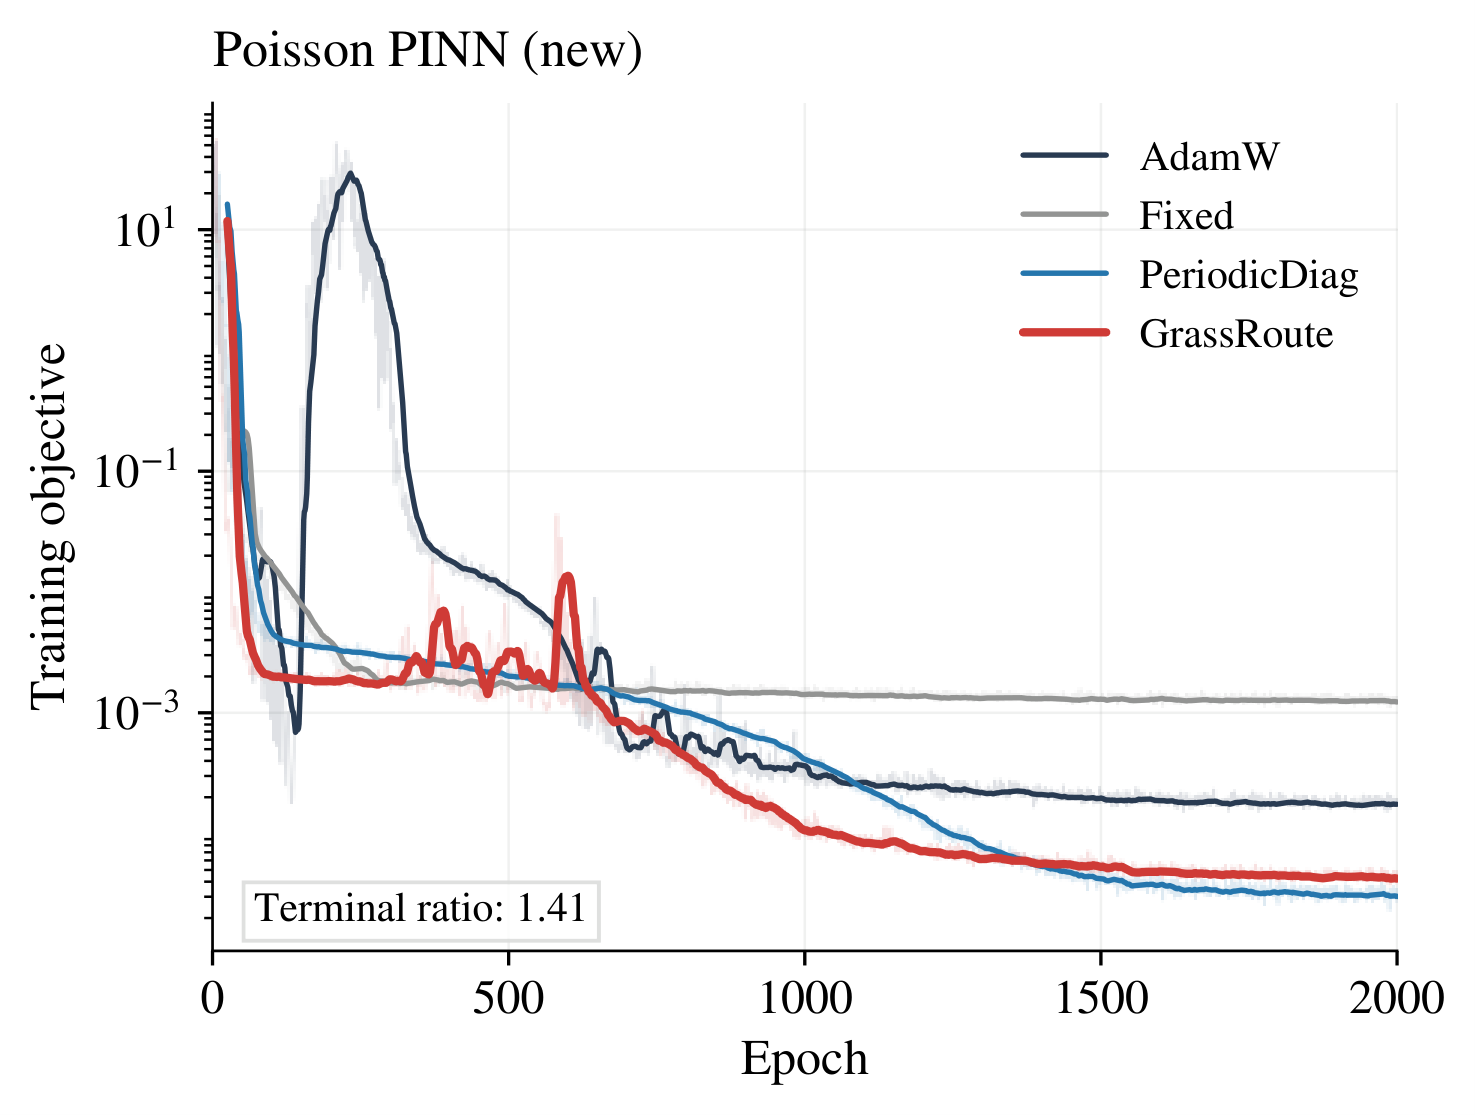
\includegraphics[width=.64\linewidth]{figures/fig_core_loss_poisson_control.png}
\caption{Poisson loss control from the independent nine-candidate validation
search, with all four selected 2000-epoch trajectories retained. Faint curves
are raw objectives and solid curves are 25-epoch trailing means. The terminal
ratio is the ratio of the final-100-epoch mean losses, GrassRoute / PeriodicDiag.
GrassRoute has lower training loss than the selected AdamW run, whereas
PeriodicDiag has the lowest loss. As with the held-out endpoints in
Table~\ref{tab:pinn-strength}, this comparison is sensitive to finite-horizon
validation selection; it does not supersede the stronger AdamW endpoint from
the original search. This control accompanies the core loss figure in the
main text without treating the protocols as interchangeable.}
\label{fig:poisson-loss-control}
\end{figure}

\subsection{Evaluation and resource conventions}
All formal comparisons use seed 42 and a predefined validation budget.
The dataset, resolution, model and training horizon are recorded with each
configuration. Test metrics refer to the final selected endpoint; shared-host
resource times include evaluation and checkpointing. Completion counts refer
to verified full trajectories, with queued and partial runs listed separately.

% WWW table style: three rules, bold headers, reference green highlight.
\subsection{Archived and original proposal results}
\label{app:full-results}
\begin{table}[ht]
\centering\small
\caption{Reported tuned historical summaries. Accuracy and Recall@20 are percentages. SciML reports best training loss; its historical SGD proxy is a different metric and is omitted. Values are selected historical observations, often best observed test accuracy, and are not final held-out endpoints from the extension.}
\label{tab:archive}
\reviewfit{\begin{tabular}{llrrrr}
\toprule {\bfseries Task} & {\bfseries Metric} & {\bfseries SGD-M} & {\bfseries AdamW} & {\bfseries Periodic SVD} & \cellcolor{oursbg}{\bfseries GrassRoute}\\
\midrule
Burgers / PINN  &  train loss $\downarrow$  &  --  &  .0110  &  .00327  &  \cellcolor{oursbg}.00197\\
Cora / GCN  &  acc. $\uparrow$  &  --  &  78.3  &  80.4  &  \cellcolor{oursbg}80.0\\
ogbn-arxiv / SAGE  &  acc. $\uparrow$  &  54.8  &  55.1  &  53.4  &  \cellcolor{oursbg}52.7\\
CIFAR-100 / partial  &  acc. $\uparrow$  &  73.13  &  71.36  &  --  &  \cellcolor{oursbg}73.32\\
CIFAR-100 / full  &  acc. $\uparrow$  &  --  &  71.36  &  65.6  &  \cellcolor{oursbg}59.45\\
MNIST / MLP  &  acc. $\uparrow$  &  98.65  &  98.53  &  98.36  &  \cellcolor{oursbg}98.25\\
Rotated MNIST  &  avg. acc. $\uparrow$  &  --  &  61.6  &  59.66  &  \cellcolor{oursbg}58.25\\
MovieLens / MF  &  R@20 $\uparrow$  &  17.1  &  6.1  &  6.2  &  \cellcolor{oursbg}7.5\\
\bottomrule
\end{tabular}}
\end{table}

The clear archived joint gain is the Burgers PINN: GrassRoute improves best training loss relative to both AdamW and tuned periodic SVD, with a reported 84.1\% reduction in persistent optimizer state. That is one scientific-learning family, not evidence from several independent PDE tasks. Its reported 1.78$\times$ step cost is a compute penalty accompanying the state saving. The old PDE evaluation is a residual-plus-initial-condition proxy rather than an actual solution relative error, and the boundary-condition omission limits physical interpretation (Appendix~\ref{app:audit}).

Cora is a qualified positive result against AdamW, but tuned periodic SVD is slightly better. The CNN partial variant improves AdamW by 1.96 percentage points and tuned SGD by only 0.19 points in the archived single run. Its state is 88.19 MB versus AdamW's 89.76 MB, saving only about 1.8\%. Full routing reduces state to 8.68 MB but loses 11.91 accuracy points relative to AdamW. These are distinct accuracy--memory trade-offs, not a CNN joint win. The graph-arxiv, MLP, recommendation, and continual-learning results do not establish a robust GrassRoute advantage. Archived ViT has complete AdamW and periodic-SVD trajectories but no complete GrassRoute endpoint.

The old broad claims about a single geometric predictor are not retained. Captured energy is not an eigengap, the recorded consecutive-basis angle is not oracle error, and nominal rank sweeps did not always change the parameter-group ranks. These issues motivate new controlled diagnostics and explicit provenance rather than retrospective reclassification of negative results.

\subsection{Validation-selected original proposal matrix}
The current extension contains 117 completed formal task--method runs out of 162, with 19 configurations complete across all six methods. The original queue was stopped after 117 completed runs; unfinished cells are marked -- and have not been used to declare a winner. The completed extension comparisons do not yet establish a new case that improves on both AdamW and periodic SVD. Against AdamW alone, the completed paired scores favor GrassRoute on PubMed / SAGE; this is a qualified comparison, not an all-baseline win. All values are final held-out test scores of the validation-selected configuration; classification and Recall@20 are percentages.

% WWW table style: three rules, bold headers, reference green highlight.
\begin{table}[htbp]
\centering\scriptsize
\setlength{\tabcolsep}{3pt}
\caption{Validation-selected extension, seed 42. Formal budgets are 1000 epochs for classification and recommendation, 2000 for MLP and scientific learning. Accuracy and Recall@20 are percentages; scientific results report solution relative error. Bold marks a best score only after all six methods have completed. -- denotes an unfinished formal comparison. GrassRoute uses diagonal moment transport; the periodic comparator retains its old second-moment diagonal at refreshes. A transport-corrected follow-up is reported separately. SubTrack++ is the pinned official implementation.}
\label{tab:extension}
\reviewfit{\begin{tabular}{llrrrrrr}
\toprule {\bfseries Task / model} & {\bfseries Metric} & {\bfseries SGD-M} & {\bfseries AdamW} & {\bfseries Fixed} & {\bfseries Periodic} & \cellcolor{oursbg}{\bfseries GrassRoute} & {\bfseries SubTrack++}\\
\midrule
MNIST / MLP  &  Acc. $\uparrow$  &  \textbf{98.65}  &  98.13  &  97.25  &  97.82  &  \cellcolor{oursbg}97.90 &  97.18 \\
ResNet-18 / CIFAR-10  &  Acc. $\uparrow$  &  \textbf{95.06}  &  94.50  &  91.43  &  92.85  &  \cellcolor{oursbg}89.99 &  93.25 \\
ResNet-18 / CIFAR-100  &  Acc. $\uparrow$  &  77.02  &  73.12  &  --  &  68.35  &  \cellcolor{oursbg}-- &  -- \\
ResNet-18 / Tiny-ImageNet  &  Acc. $\uparrow$  &  --  &  --  &  --  &  --  &  \cellcolor{oursbg}-- &  -- \\
ResNet-18 / ImageNet-100  &  Acc. $\uparrow$  &  --  &  --  &  --  &  --  &  \cellcolor{oursbg}-- &  -- \\
ViT-Tiny / CIFAR-100  &  Acc. $\uparrow$  &  --  &  --  &  --  &  --  &  \cellcolor{oursbg}-- &  -- \\
ViT-Tiny / Tiny-ImageNet  &  Acc. $\uparrow$  &  --  &  --  &  --  &  --  &  \cellcolor{oursbg}-- &  -- \\
ViT-Tiny / ImageNet-100  &  Acc. $\uparrow$  &  --  &  --  &  --  &  --  &  \cellcolor{oursbg}-- &  -- \\
Cora / SAGE  &  Acc. $\uparrow$  &  \textbf{79.50}  &  78.30  &  43.10  &  79.10  &  \cellcolor{oursbg}78.00 &  76.70 \\
CiteSeer / SAGE  &  Acc. $\uparrow$  &  \textbf{69.70}  &  68.10  &  30.80  &  68.70  &  \cellcolor{oursbg}67.10 &  67.10 \\
PubMed / SAGE  &  Acc. $\uparrow$  &  \textbf{77.40}  &  74.20  &  59.50  &  77.10  &  \cellcolor{oursbg}76.00 &  75.60 \\
ogbn-arxiv / SAGE  &  Acc. $\uparrow$  &  53.78  &  55.05  &  32.57  &  53.16  &  \cellcolor{oursbg}51.86 &  \textbf{55.46} \\
Poisson / PINN  &  Rel.$L_2\downarrow$  &  1.0000  &  {\boldmath $9.28\!\times\!10^{-5}$}  &  $9.95\!\times\!10^{-4}$  &  $2.99\!\times\!10^{-4}$  &  \cellcolor{oursbg}$1.26\!\times\!10^{-4}$ &  $4.03\!\times\!10^{-4}$ \\
Forced Burgers / PINN  &  Rel.$L_2\downarrow$  &  0.0132  &  {\boldmath $1.49\!\times\!10^{-3}$}  &  $6.41\!\times\!10^{-3}$  &  $1.90\!\times\!10^{-3}$  &  \cellcolor{oursbg}$2.08\!\times\!10^{-3}$ &  $1.55\!\times\!10^{-3}$ \\
Darcy / DeepONet  &  Rel.$L_2\downarrow$  &  0.0867  &  \textbf{0.0199}  &  0.0223  &  0.0370  &  \cellcolor{oursbg}0.0380 &  0.1087 \\
Burgers operator / FNO  &  Rel.$L_2\downarrow$  &  0.0145  &  {\boldmath $7.82\!\times\!10^{-3}$}  &  0.0177  &  0.0148  &  \cellcolor{oursbg}0.0201 &  0.0141 \\
MovieLens-1M / MF  &  R@20 $\uparrow$  &  10.59  &  \textbf{12.36}  &  11.77  &  12.35  &  \cellcolor{oursbg}12.25 &  12.33 \\
Amazon Books subset / MF  &  R@20 $\uparrow$  &  0.00  &  \textbf{1.25}  &  0.85  &  0.90  &  \cellcolor{oursbg}0.95 &  0.75 \\
Yelp subset / MF  &  R@20 $\uparrow$  &  0.20  &  \textbf{2.30}  &  1.90  &  2.00  &  \cellcolor{oursbg}1.45 &  1.95 \\
Rotated MNIST / MLP  &  Acc. $\uparrow$  &  --  &  --  &  --  &  --  &  \cellcolor{oursbg}-- &  -- \\
Split CIFAR-100 / ResNet-18  &  Acc. $\uparrow$  &  --  &  --  &  --  &  --  &  \cellcolor{oursbg}-- &  -- \\
\bottomrule
\end{tabular}}
\end{table}


The original manifest spans every proposed task/dataset with representative models, rather than the full dataset--architecture--rank Cartesian product. Its 27 configurations include three input dimensions for both matrix and low-rank regression, MNIST, four CNN datasets, three ViT datasets, four graph datasets, four scientific tasks, three recommendation datasets, and two continual-learning protocols. Completed runs use full epochs and save restartable checkpoints and all epoch records. Three learning rates per method are screened on validation data before a fresh formal run. Dataset sources, actual ranks, hyperparameters, and source hashes are recorded with each result. The high-cost queue was stopped after 117 completed cells; the rest remain visibly pending. Appendix~\ref{app:audit} defines the tasks and selection budgets precisely.

% WWW table style: three rules, bold headers, reference green highlight.
\begin{table}[t]\centering\footnotesize
\caption{\textbf{Scientific-learning validation and test endpoints.} Complete 2000-epoch formal runs from the original proposal extension, selected on validation data. All entries are solution relative error. Initial validation denotes the first stored validation checkpoint; models and tasks follow the versioned protocol.}
\label{tab:new-sciml}
\setlength{\tabcolsep}{5pt}
\reviewfit{\begin{tabular}{lrrrr}
\toprule {\bfseries Task} & {\bfseries Method} & {\bfseries Initial val.} & {\bfseries Final val.} & {\bfseries Final test}\\\midrule
Poisson / PINN  &  SGD-M  &  0.4309  &  1  &  1\\
Poisson / PINN  &  AdamW  &  2.481  &  $9.19\times10^{-5}$  &  $9.28\times10^{-5}$\\
Poisson / PINN  &  Fixed  &  0.7925  &  $9.79\times10^{-4}$  &  $9.95\times10^{-4}$\\
Poisson / PINN  &  Periodic SVD  &  0.4188  &  $2.92\times10^{-4}$  &  $2.99\times10^{-4}$\\
\rowcolor{oursbg}Poisson / PINN  & \textbf{GrassRoute} &  0.4188  &  $1.25\times10^{-4}$  &  $1.26\times10^{-4}$\\
Poisson / PINN  &  SubTrack++  &  0.5623  &  $3.94\times10^{-4}$  &  $4.03\times10^{-4}$\\
Forced Burgers / PINN  &  SGD-M  &  0.8454  &  0.01289  &  0.01316\\
Forced Burgers / PINN  &  AdamW  &  2.568  &  0.001492  &  0.001489\\
Forced Burgers / PINN  &  Fixed  &  0.4933  &  0.006064  &  0.006414\\
Forced Burgers / PINN  &  Periodic SVD  &  0.4933  &  0.001853  &  0.001898\\
\rowcolor{oursbg}Forced Burgers / PINN  & \textbf{GrassRoute} &  0.4933  &  0.001953  &  0.002079\\
Forced Burgers / PINN  &  SubTrack++  &  0.8114  &  0.001515  &  0.001549\\
Darcy / DeepONet  &  SGD-M  &  0.7469  &  0.08382  &  0.08672\\
Darcy / DeepONet  &  AdamW  &  2.201  &  0.01937  &  0.01989\\
Darcy / DeepONet  &  Fixed  &  0.5206  &  0.02219  &  0.02226\\
Darcy / DeepONet  &  Periodic SVD  &  0.5206  &  0.03552  &  0.03698\\
\rowcolor{oursbg}Darcy / DeepONet  & \textbf{GrassRoute} &  0.4898  &  0.03734  &  0.03799\\
Darcy / DeepONet  &  SubTrack++  &  0.599  &  0.1036  &  0.1087\\
Burgers operator / FNO  &  SGD-M  &  0.9935  &  0.01471  &  0.01447\\
Burgers operator / FNO  &  AdamW  &  0.4612  &  0.00797  &  0.007823\\
Burgers operator / FNO  &  Fixed  &  0.7662  &  0.01922  &  0.01772\\
Burgers operator / FNO  &  Periodic SVD  &  0.7662  &  0.01526  &  0.01476\\
\rowcolor{oursbg}Burgers operator / FNO  & \textbf{GrassRoute} &  0.7062  &  0.02147  &  0.02013\\
Burgers operator / FNO  &  SubTrack++  &  0.7643  &  0.01422  &  0.01406\\
\bottomrule\end{tabular}}
\end{table}


New task coverage is evidence only when the formal comparison completes. A lower parameter-state cost can remain useful without a test-metric win; conversely, an isolated lower error does not establish a practical advantage without accounting for state and time. We therefore retain all completed baselines, including strong SGD and fixed-routing outcomes, and report shared-host resource measurements separately from accuracy. The current finite hyperparameter search and one-seed protocol do not support statistical-significance claims or exhaustive optimizer rankings.

\subsection{Focused exploratory follow-up after scope reduction}
\label{app:focused-followup}
The original 162-cell plan was stopped after 117 completed runs. The
remaining cells are retained as unfinished, including partial CIFAR-100
trajectories; they are not interpreted as full-budget endpoints. To test
the proposed tracking mechanism with less computation, we froze a separate
three-condition rotating rank-four regression stream before inspecting its
formal outcomes. Each method used four equal-budget validation candidates
and a new 1500-step run; Table~\ref{tab:focused-regression} includes all
conditions and comparators. GrassRoute's smaller subspace-angle error in
the drifting conditions did not yield a lower prediction MSE than the
strongest baselines. The Cora GCN check is motivated by the prior Cora
GraphSAGE result, so it is an exploratory architecture replication on the
same dataset. Its full six-method matrix is in Table~\ref{tab:focused-gcn}.
\begin{table*}[t]\centering\footnotesize
\caption{\textbf{Exploratory drifting-regression controls.} A rank-four
teacher in $\mathbb{R}^{16\times64}$ rotates at the stated radians per
update; stationary is the negative control. Entries are mean independent
test MSE over the last 20\% of 1500 fresh steps after four equal-budget
validation candidates per method. All conditions and outcomes are retained.
Seed 42; lower is better. State reduction compares persistent GrassRoute
optimizer state with AdamW. This synthetic stream is distinct from
public-data generalization.}
\label{tab:focused-regression}
\setlength{\tabcolsep}{6pt}
\begin{tabular}{lrrrrrr}\toprule
Drift & SGD-M & AdamW & Fixed & Periodic SVD & GrassRoute & State reduction \\ \midrule
$0$ & $2.346\times10^{-5}$ & $9.139\times10^{-4}$ & $3.705\times10^{-5}$ & $3.425\times10^{-5}$ & \cellcolor{oursbg}$4.235\times10^{-5}$ & 68.8\% \\
$0.005$ & $3.448\times10^{-4}$ & $4.767\times10^{-3}$ & $1.149\times10^{-3}$ & $6.947\times10^{-4}$ & \cellcolor{oursbg}$7.778\times10^{-4}$ & 68.8\% \\
$0.020$ & $1.315\times10^{-3}$ & $1.002\times10^{-2}$ & $1.648\times10^{-2}$ & $1.694\times10^{-2}$ & \cellcolor{oursbg}$2.395\times10^{-1}$ & 68.8\% \\
\bottomrule\end{tabular}\end{table*}

\begin{table}[t]\centering\footnotesize
\caption{\textbf{Focused Cora GCN architecture check.} Nine 100-epoch
validation candidates per method and a fresh 1000-epoch formal run.
Final public-test accuracy (\%) on the Planetoid split, seed 42.
All six methods and incomplete cells are shown. This reuses Cora and
is an architecture replication, not a new dataset-family win.}
\label{tab:focused-gcn}
\setlength{\tabcolsep}{4pt}
\begin{tabular}{lr}\toprule Method & Test accuracy \\ \midrule
SGD & 81.10 \\
AdamW & 78.50 \\
Fixed & 21.40 \\
Periodic SVD & 80.50 \\
GrassRoute & \cellcolor{oursbg}80.30 \\
SubTrack++ & 78.60 \\
\bottomrule\end{tabular}\end{table}


We additionally froze the seed-42 validation-selected hyperparameters from
the original Cora GraphSAGE and SMS studies, then reran three new
initializations (43--45) per method on each unchanged public split. These
replications use four prespecified core comparators and retain all endpoints
in Tables~\ref{tab:focused-cora-replication}
and~\ref{tab:focused-sms-replication}; they do not add independent datasets.
A numerical failure at a frozen hyperparameter is kept as such and does not
trigger a test-selected replacement.
\begin{table*}[t]\centering\footnotesize
\caption{\textbf{Cora GraphSAGE fixed-hyperparameter seed replication.} Three fresh 1000-epoch runs use
hyperparameters frozen from the original seed-42 validation selection.
The public split and architecture are fixed; seeds 43--45 vary
initialization and stochastic training. Accuracy or macro-F1 is in
percent. Mean and sample standard deviation are descriptive.
Persistent optimizer state is in decimal MB. All endpoints are shown;
\emph{fail} denotes a retained numerical failure.}
\label{tab:focused-cora-replication}
\setlength{\tabcolsep}{7pt}
\begin{tabular}{lrrrrr}\toprule
Method & Seed 43 & Seed 44 & Seed 45 & Mean $\pm$ SD & State MB \\ \midrule
SGD & 79.30 & 79.40 & 79.00 & 79.23 $\pm$ 0.21 & 1.475 \\
AdamW & 78.10 & 77.50 & 77.30 & 77.63 $\pm$ 0.42 & 2.950 \\
Periodic SVD & 78.10 & \emph{fail} & 78.60 & -- & 0.207 \\
GrassRoute & \cellcolor{oursbg}78.30 & \cellcolor{oursbg}75.70 & \cellcolor{oursbg}76.70 & \cellcolor{oursbg}76.90 $\pm$ 1.31 & 0.207 \\
\bottomrule\end{tabular}\end{table*}

\begin{table*}[t]\centering\footnotesize
\caption{\textbf{SMS text classification fixed-hyperparameter seed replication.} Three fresh 1000-epoch runs use
hyperparameters frozen from the original seed-42 validation selection.
The public split and architecture are fixed; seeds 43--45 vary
initialization and stochastic training. Accuracy or macro-F1 is in
percent. Mean and sample standard deviation are descriptive.
Persistent optimizer state is in decimal MB. All endpoints are shown;
\emph{fail} denotes a retained numerical failure.}
\label{tab:focused-sms-replication}
\setlength{\tabcolsep}{7pt}
\begin{tabular}{lrrrrr}\toprule
Method & Seed 43 & Seed 44 & Seed 45 & Mean $\pm$ SD & State MB \\ \midrule
SGD & 96.30 & 94.63 & 94.60 & 95.18 $\pm$ 0.97 & 0.525 \\
AdamW & 95.76 & 95.20 & 95.48 & 95.48 $\pm$ 0.28 & 1.050 \\
Periodic SVD & 93.94 & 94.29 & 94.63 & 94.29 $\pm$ 0.35 & 0.071 \\
GrassRoute & \cellcolor{oursbg}94.29 & \cellcolor{oursbg}95.64 & \cellcolor{oursbg}94.29 & \cellcolor{oursbg}94.74 $\pm$ 0.78 & 0.137 \\
\bottomrule\end{tabular}\end{table*}



% WWW table style: three rules, bold headers, reference green highlight.
\begin{table}[htbp]\centering\scriptsize
\caption{All completed paired extension endpoints: state retained relative to AdamW, and final test metrics. Lower state is beneficial; metric direction is explicit. These are the original versioned periodic endpoints, not the transport-corrected follow-up. Wall time is not encoded as isolated speed.}
\label{tab:state-quality}
\reviewfit{\begin{tabular}{lrrrr}\toprule {\bfseries Task} & {\bfseries State / AdamW} & {\bfseries AdamW} & \cellcolor{oursbg}{\bfseries GrassRoute} & {\bfseries Periodic}\\\midrule
Matrix reg. / 128 $\downarrow$  &  62.5\%  &  $1.07\!\times\!10^{-4}$  &  \cellcolor{oursbg}0.484 &  $1.07\!\times\!10^{-4}$\\
Matrix reg. / 256 $\downarrow$  &  56.2\%  &  $1.12\!\times\!10^{-4}$  &  \cellcolor{oursbg}0.341 &  $1.12\!\times\!10^{-4}$\\
Matrix reg. / 512 $\downarrow$  &  53.1\%  &  $1.31\!\times\!10^{-4}$  &  \cellcolor{oursbg}0.366 &  $1.31\!\times\!10^{-4}$\\
Low-rank reg. / 128 $\downarrow$  &  62.5\%  &  $1.04\!\times\!10^{-4}$  &  \cellcolor{oursbg}0.023 &  $1.04\!\times\!10^{-4}$\\
Low-rank reg. / 256 $\downarrow$  &  56.2\%  &  $1.19\!\times\!10^{-4}$  &  \cellcolor{oursbg}0.00962 &  $1.19\!\times\!10^{-4}$\\
Low-rank reg. / 512 $\downarrow$  &  53.1\%  &  $1.32\!\times\!10^{-4}$  &  \cellcolor{oursbg}0.0194 &  $1.32\!\times\!10^{-4}$\\
MNIST / MLP $\uparrow$  &  6.5\%  &  98.13  &  \cellcolor{oursbg}97.90 &  97.82\\
ResNet-18 / CIFAR-10 $\uparrow$  &  10.4\%  &  94.50  &  \cellcolor{oursbg}89.99 &  92.85\\
Cora / SAGE $\uparrow$  &  7.0\%  &  78.30  &  \cellcolor{oursbg}78.00 &  79.10\\
CiteSeer / SAGE $\uparrow$  &  6.6\%  &  68.10  &  \cellcolor{oursbg}67.10 &  68.70\\
PubMed / SAGE $\uparrow$  &  8.5\%  &  74.20  &  \cellcolor{oursbg}76.00 &  77.10\\
ogbn-arxiv / SAGE $\uparrow$  &  16.1\%  &  55.05  &  \cellcolor{oursbg}51.86 &  53.16\\
Poisson / PINN $\downarrow$  &  14.2\%  &  $9.28\!\times\!10^{-5}$  &  \cellcolor{oursbg}$1.26\!\times\!10^{-4}$ &  $2.99\!\times\!10^{-4}$\\
Forced Burgers / PINN $\downarrow$  &  14.5\%  &  0.00149  &  \cellcolor{oursbg}0.00208 &  0.0019\\
Darcy / DeepONet $\downarrow$  &  16.5\%  &  0.0199  &  \cellcolor{oursbg}0.038 &  0.037\\
Burgers operator / FNO $\downarrow$  &  27.4\%  &  0.00782  &  \cellcolor{oursbg}0.0201 &  0.0148\\
MovieLens-1M / MF $\uparrow$  &  25.3\%  &  12.36  &  \cellcolor{oursbg}12.25 &  12.35\\
Amazon Books subset / MF $\uparrow$  &  25.1\%  &  1.25  &  \cellcolor{oursbg}0.95 &  0.90\\
Yelp subset / MF $\uparrow$  &  25.1\%  &  2.30  &  \cellcolor{oursbg}1.45 &  2.00\\
\bottomrule\end{tabular}}\end{table}


\IfFileExists{figures/strength_graph_table.tex}{% WWW table style: three rules, bold headers, reference green highlight.
\begin{table}[htbp]\centering\scriptsize\setlength{\tabcolsep}{3pt}
\caption{Independent Planetoid follow-up: nine 100-epoch validation candidates per method, then 1000 fresh formal epochs, seed 42. All accuracies are final public-test percentages; -- indicates unfinished training. The periodic method now transports both moments. SubTrack++ is the same pinned official implementation. These are transductive graph experiments.}
\label{tab:graph-strength}
\reviewfit{\begin{tabular}{lrrrrrr}\toprule {\bfseries Task} & {\bfseries SGD-M} & {\bfseries AdamW} & {\bfseries Fixed} & {\bfseries PeriodicDiag} & \cellcolor{oursbg}{\bfseries GrassRoute} & {\bfseries SubTrack++}\\\midrule
Cora / SAGE  &  \textbf{79.70}  &  77.50  &  39.10  &  77.70  &  \cellcolor{oursbg}78.60 &  77.30\\
CiteSeer / SAGE  &  68.80  &  67.40  &  36.90  &  \textbf{69.10}  &  \cellcolor{oursbg}68.40 &  64.90\\
PubMed / SAGE  &  \textbf{76.90}  &  74.80  &  53.90  &  76.80  &  \cellcolor{oursbg}76.60 &  76.20\\
\bottomrule\end{tabular}}\end{table}
}{}

\subsection{Accuracy--state evidence and independent follow-up}
\label{sec:strength-followup}
The practical claim is specific: retaining adaptive state only in selected
directions can reduce persistent optimizer memory while preserving useful
prediction quality, and continuous tracking can average noisy directional
information. It does not require the same optimizer to win every final-error
comparison. We expose both the favorable and unfavorable cases.

\paragraph{Measured state versus final prediction quality.}
On PubMed the original extension obtains 76.0\% with GrassRoute versus
74.2\% with AdamW, retaining 87,576 versus 1,031,216 state bytes: a 91.5\%
reduction and a 1.8 percentage-point accuracy gain in the single paired run.
The periodic implementation is more accurate at 77.1\% with the same state
cost. On all-user MovieLens, GrassRoute retains 25.3\% of AdamW's state and
obtains 12.247\% versus 12.363\% Recall@20, a 0.116 percentage-point loss.
This is a measured memory--quality trade-off, not a significance or
noninferiority claim. On Poisson its relative solution error is
$1.255\times10^{-4}$ versus $2.987\times10^{-4}$ for the original periodic
implementation at the same persistent state cost, but AdamW is more accurate.
Table~\ref{tab:state-quality} retains every completed paired task, including
the unfavorable regression and operator-learning results.

\paragraph{Actual-implementation tracking test.}
We run the routed optimizer code on Gaussian gradient matrices with a known
rotating population covariance, using rank 4 in dimension 64, signal/tail
eigenvalues $1$ and $0.03$, and 16 or 128 gradient rows per update. The four
rotation rates are $0,0.001,0.005,0.02$ radians per step. All methods start
from the same random frame and observe the same 2000 matrices. We compare
GrassRoute at a fixed $\rho=3$, its no-momentum ablation, a fixed router,
and transport-corrected instantaneous SVD refreshes at periods 5, 25 and 100.
The target projector is known analytically; no compressed-Gram proxy is used.
Error is measured \emph{before} updating on the current gradient, preventing
a freshly computed SVD from being evaluated only on its fitting batch.
\input{figures/strength_tracking_summary}
\input{figures/tracking_resource_table}
\IfFileExists{figures/strength_tracking_table.tex}{\input{figures/strength_tracking_table}}{}

\paragraph{Stronger smoothing controls and a faster-drift stress test.}
Instantaneous SVD does not average sample noise; that is a meaningful
property of that baseline; full-covariance estimators can also average noise. A second,
independently recorded protocol therefore adds normalized full-covariance EMA
estimators with decays $0.9$ and $0.99$, each refreshed every 5 or 25 steps.
It retains every original condition and adds rotation rate $0.1$ at both row
counts. The full $64\times64$ covariance is stored and counted. The same
moment transport, starting frame, stream and pre-update metric are used.
This control can exploit temporal smoothing without requiring Grassmann
momentum, at an additional state cost.
\IfFileExists{figures/strength_tracking_ema_summary.tex}{\input{figures/strength_tracking_ema_summary}}{}

\IfFileExists{figures/strength_tracking_ema_table.tex}{\input{figures/strength_tracking_ema_table}}{}

\paragraph{Independent, larger validation budget on exact-solution PINNs.}
We return to the scientific-learning family motivated by the archived
Burgers result and include \emph{both} exact-solution PINNs, rather than
searching only the favorable task. Each of AdamW, fixed routing,
\textsc{PeriodicDiag}, and GrassRoute receives nine 100-epoch validation
screening runs. AdamW searches nine geometrically spaced learning rates from
$10^{-4}$ to $0.03$. Each routed method searches learning rates
$\{0.001,0.003,0.01\}$, crossed with a method-specific parameter:
residual-rate ratios $\{0.3,1,3\}$ for fixed routing; refresh periods
$\{5,25,100\}$ for \textsc{PeriodicDiag}; and tracking rates
$\{0.3,1,3\}$ for GrassRoute. All candidates, including divergence records,
are retained. Selection uses final validation relative solution error;
the selected configuration is trained afresh for 2000 full epochs, and test
error is evaluated once at the end. Parameter initialization and collocation
streams are paired. The protocol and source hash were saved before the runs.
This follow-up changes the search budget and periodic transport, so its
endpoints remain separate from the 162-comparison proposal extension.
\input{figures/strength_pinn_summary}
On Poisson, GrassRoute's selected relative solution error is
$6.70\times10^{-5}$ at 0.0379 MB of persistent optimizer state, versus
$9.52\times10^{-4}$ at 0.2673 MB for the independently selected AdamW
configuration. This favorable comparison is selection-sensitive: the original,
smaller search already found an AdamW endpoint of $9.28\times10^{-5}$,
and \textsc{PeriodicDiag} in the new search achieves $4.90\times10^{-5}$.
On forced Burgers, AdamW remains better than GrassRoute. More screening
candidates do not guarantee better long-horizon selection when screening
lasts only 100 epochs; the complete endpoints, not only favorable pairs,
are shown below.
\IfFileExists{figures/strength_pinn_table.tex}{\input{figures/strength_pinn_table}}{}

\paragraph{Checking the graph result with equal, expanded search budgets.}
A separate follow-up tests Cora, CiteSeer and PubMed against all six methods,
including corrected periodic transport and official SubTrack++. Each method
receives nine 100-epoch validation candidates and 1000 fresh formal epochs.
GrassRoute crosses three learning rates with tracking rates
$\{0.3,1,3\}$; fixed routing searches residual-rate ratios, corrected periodic
routing searches refresh intervals, and official SubTrack++ searches its
initial geodesic step. AdamW and SGD each search nine learning rates. The
protocol records every candidate before training, uses paired model/dropout
streams and the public graph splits, and retains every selected endpoint.
These transductive results test optimizer performance and do not validate the
iid assumptions of the generalization theorem.
Numerical failures, bounded process retries, and a device-only CPU adapter
are recorded separately; they do not alter the nine unique hyperparameters or
permit test-driven fallback (Appendix~\ref{app:numerical-recovery}).
\input{figures/strength_graph_summary}


% WWW table style: three rules, bold headers, reference green highlight.
\subsection{Complete new public-data suite}
\label{app:new-task-full}
The six new tasks are retained as a complete evaluation set. The suite was
motivated by the geometric hypothesis after examining the earlier archive;
it is a follow-up study rather than an independent confirmation of universal
optimizer superiority. A main-text subset is identified by the rule in
Section~\ref{sec:new-public-tasks}; this appendix retains all six tasks and
all methods regardless of their ranking. No unsuccessful run is deleted
after observing its test result.

\begin{table}[htbp]\centering\small
\caption{New-task data and primary metrics. Preprocessing fits the training
split only. Counts are actual prepared examples, not nominal dataset sizes.}
\reviewfit{\begin{tabular}{lrrrl}\toprule {\bfseries Task} & {\bfseries Train} & {\bfseries Validation} & {\bfseries Test} & {\bfseries Primary metric}\\\midrule
20 Newsgroups  &  9051  &  2263  &  7532  &  Macro-F1 $\uparrow$\\
SMS Spam (deduplicated)  &  3612  &  774  &  774  &  Macro-F1 $\uparrow$\\
Adult  &  26048  &  6513  &  16281  &  AUROC $\uparrow$\\
Spambase  &  3220  &  690  &  691  &  AUROC $\uparrow$\\
Optdigits denoising  &  3058  &  765  &  1797  &  Pixel MSE $\downarrow$\\
Optdigits completion  &  3058  &  765  &  1797  &  Missing-pixel MSE $\downarrow$\\
\bottomrule\end{tabular}}\end{table}

\paragraph{Text.}
20 Newsgroups uses the official by-date train/test split through the
scikit-learn loader, with headers, footers and quotes removed
\cite{sklearn20newsdata}. A stratified 20\% of the official training set is
reserved for validation. TF-IDF uses a vocabulary of at most 2048 terms,
minimum document frequency 2, maximum document frequency 0.95, sublinear
term frequency and row normalization; its vocabulary and inverse document
frequencies fit only the training documents. Official test documents,
including empty texts and exact-text overlaps in the released corpus, are
retained and those counts are recorded; exact-text independence is not
asserted. SMS Spam \cite{uci2011sms} removes exact stripped-message duplicates
and conflicting duplicate labels before a stratified 70/15/15 split. It uses
the same TF-IDF parameters. Both text models use a 64-unit ReLU hidden layer,
dropout 0.1, and a linear classifier. Sparse inputs remain sparse in the first
matrix product. Macro-F1, rather than majority-class accuracy, is the primary
selection metric; predictions use the fixed argmax rule.

\paragraph{Structured data.}
Adult \cite{uci1996adult} retains its official test set and reserves 20\% of
its training rows for stratified validation. Continuous features are
standardized with training statistics; categories are training-fitted one-hot
features, unknown categories are ignored and missing categories are explicit.
Spambase \cite{uci1999spambase} uses a stratified 70/15/15 split and training
standardization. Both models have 128 and 64 ReLU units, dropout 0.1 after
the first hidden layer, and two output logits. The primary metric is AUROC;
accuracy, macro-F1 and cross-entropy are retained as secondary diagnostics.

\paragraph{Inverse imaging.}
The Optdigits corpus \cite{uci1998optdigits} preserves its official
writer-disjoint test set, with 20\% of the original training set reserved
for stratified validation. The 64 pixel features are divided by 16. The
denoising task adds independent Gaussian noise with standard deviation 0.3
and clips corrupted inputs to $[0,1]$. The completion task independently
masks half the pixels and concatenates the visibility mask to the input.
Training uses fresh corruptions on every full epoch; validation and testing
use fixed independent corruptions. The encoder--decoder widths are
128--32--128, with tanh hidden activations and sigmoid output. Denoising
optimizes all-pixel MSE. Completion optimizes missing-pixel MSE; observed
pixels are copied when computing full-image reconstruction MSE and PSNR.
The two tasks do not constitute separate independent image datasets.

\paragraph{Search and state accounting.}
Ranks start at 8 and are capped below the input dimension and at half the
output dimension. Small matrices and biases use full Adam fallback in routed
methods. All weight decays are zero. AdamW searches learning rates
$\{0.0003,0.0005,0.001,0.002,0.003,0.005,0.01,0.02,0.03\}$;
SGD-M searches nine geometrically spaced rates from $0.001$ to 3, with
momentum 0.9. Routed methods cross rates $\{0.001,0.003,0.01\}$ with
residual-rate ratios $\{1,10,100\}$. GrassRoute tracking rates
$\{0.3,1,3\}$ and periodic intervals $\{5,25,100\}$ are assigned in a
balanced cyclic design across those nine cells, not exhaustively crossed.
Official SubTrack++ crosses the same three parameter rates with initial
subspace steps $\{0.1,1,3\}$ and uses the device-only CPU adapter described
above. Adaptive moments use $\beta_1=0.9,\beta_2=0.999$; GrassRoute uses
routing momentum 0.9 and diagonal transport. Fixed and periodic comparators
retain no unused routing momentum. Thin SVD uses a double-precision retry
only if its single-precision decomposition raises a linear algebra error.
Persistent state is measured from allocated optimizer storage, including the
official projector state. Shared-host CPU wall times are not isolated speed
measurements.

All screening runs use 200 complete epochs; final validation selects a
configuration, which is retrained afresh for 1000 epochs before a single
held-out test evaluation. Optimizer random initialization is isolated from
dropout/corruption streams. Restartable checkpoints retain model, optimizer
and random states. Every candidate, numerical failure, full trajectory,
source hash and endpoint remains in the ledger. The frozen manifest is
\path{revision/newtask_results/protocol.json}; the checked outcome ledger is
\path{revision/newtask_status.json}. These new runs do not inflate the
original 162-comparison completion count.

% WWW table style: three rules, bold headers, reference green highlight.
\begin{table}[htbp]\centering\scriptsize\setlength{\tabcolsep}{3pt}
\caption{Complete frozen new-task matrix, seed 42. Nine 200-epoch validation candidates per method, followed by 1000 fresh full epochs. Macro-F1 and AUROC are percentages; image tasks report MSE (missing pixels for inpainting). -- means unfinished or numerically failed, with failures retained in the ledger. Best endpoints are bold only after all six methods complete.}
\label{tab:newtasks-full}
\reviewfit{\begin{tabular}{llrrrrrr}\toprule {\bfseries Task} & {\bfseries Metric} & {\bfseries SGD-M} & {\bfseries AdamW} & {\bfseries Fixed} & {\bfseries Thin SVD} & \cellcolor{oursbg}{\bfseries GrassRoute} & {\bfseries SubTrack++}\\\midrule
Optdigits / denoising  &  MSE $\downarrow$  &  0.0236  &  0.0187  &  0.0325  &  0.0241  &  \cellcolor{oursbg}0.0249 &  \textbf{0.0178}\\
Optdigits / inpainting  &  MSE $\downarrow$  &  0.0412  &  \textbf{0.0296}  &  0.0507  &  0.0379  &  \cellcolor{oursbg}0.0429 &  0.0314\\
Spambase / MLP  &  AUC $\uparrow$  &  \textbf{97.87}  &  97.62  &  97.41  &  97.58  &  \cellcolor{oursbg}97.55 &  97.80\\
Adult / MLP  &  AUC $\uparrow$  &  89.29  &  88.91  &  90.75  &  \textbf{91.23}  &  \cellcolor{oursbg}90.27 &  89.14\\
SMS / TF-IDF MLP  &  F1 $\uparrow$  &  \textbf{95.48}  &  \textbf{95.48}  &  46.69  &  94.29  &  \cellcolor{oursbg}94.63 &  95.40\\
20 News / TF-IDF MLP  &  F1 $\uparrow$  &  \textbf{54.33}  &  50.95  &  52.96  &  53.49  &  \cellcolor{oursbg}52.31 &  50.38\\
\bottomrule\end{tabular}}\end{table}

% WWW table style: three rules, bold headers, reference green highlight.
{\scriptsize\setlength{\tabcolsep}{3pt}
\begin{longtable}{llrrrrr}
\caption{All classification secondary endpoints and state costs in the new suite. Text configurations were selected by macro-F1 and tabular configurations by AUROC, never by the secondary test metrics. Accuracy, F1 and AUC are percentages; cross-entropy is unscaled; persistent state is decimal MB. -- means unfinished or inapplicable.}\label{tab:newtasks-secondary}\\
\toprule {\bfseries Task} & {\bfseries Method} & {\bfseries Accuracy} & {\bfseries Macro-F1} & {\bfseries AUROC} & {\bfseries CE} & {\bfseries State MB}\\\midrule\endfirsthead
\toprule {\bfseries Task} & {\bfseries Method} & {\bfseries Accuracy} & {\bfseries Macro-F1} & {\bfseries AUROC} & {\bfseries CE} & {\bfseries State MB}\\\midrule\endhead
Spambase / MLP & SGD-M & 93.34 & 93.02 & 97.87 & 0.3269 & 0.063\\
Spambase / MLP & AdamW & 94.07 & 93.76 & 97.62 & 0.5338 & 0.127\\
Spambase / MLP & Fixed & 94.07 & 93.78 & 97.41 & 0.4692 & 0.021\\
Spambase / MLP & Thin SVD & 93.63 & 93.34 & 97.58 & 0.3465 & 0.021\\
\rowcolor{oursbg}Spambase / MLP & \textbf{GrassRoute} & 92.19 & 91.81 & 97.55 & 0.3459 & 0.027\\
Spambase / MLP & SubTrack++ & 93.34 & 93.02 & 97.80 & 0.4853 & 0.056\\
Adult / MLP & SGD-M & 84.15 & 77.23 & 89.29 & 0.4159 & 0.089\\
Adult / MLP & AdamW & 84.14 & 76.98 & 88.91 & 0.3993 & 0.179\\
Adult / MLP & Fixed & 85.25 & 78.59 & 90.75 & 0.3185 & 0.022\\
Adult / MLP & Thin SVD & 85.58 & 79.16 & 91.23 & 0.3067 & 0.022\\
\rowcolor{oursbg}Adult / MLP & \textbf{GrassRoute} & 84.86 & 78.31 & 90.27 & 0.3408 & 0.030\\
Adult / MLP & SubTrack++ & 83.71 & 76.94 & 89.14 & 0.4541 & 0.093\\
SMS / TF-IDF MLP & SGD-M & 98.06 & 95.48 & 99.30 & 0.0799 & 0.525\\
SMS / TF-IDF MLP & AdamW & 98.06 & 95.48 & 98.28 & 0.1752 & 1.050\\
SMS / TF-IDF MLP & Fixed & 87.60 & 46.69 & 64.97 & 0.3601 & 0.071\\
SMS / TF-IDF MLP & Thin SVD & 97.67 & 94.29 & 99.02 & 0.0952 & 0.071\\
\rowcolor{oursbg}SMS / TF-IDF MLP & \textbf{GrassRoute} & 97.80 & 94.63 & 99.08 & 0.0931 & 0.137\\
SMS / TF-IDF MLP & SubTrack++ & 98.06 & 95.40 & 97.50 & 0.1415 & 0.153\\
20 News / TF-IDF MLP & SGD-M & 55.12 & 54.33 & -- & 2.1272 & 0.530\\
20 News / TF-IDF MLP & AdamW & 51.66 & 50.95 & -- & 2.4000 & 1.060\\
20 News / TF-IDF MLP & Fixed & 54.25 & 52.96 & -- & 1.4909 & 0.074\\
20 News / TF-IDF MLP & Thin SVD & 54.30 & 53.49 & -- & 1.6752 & 0.074\\
\rowcolor{oursbg}20 News / TF-IDF MLP & \textbf{GrassRoute} & 53.21 & 52.31 & -- & 1.7997 & 0.141\\
20 News / TF-IDF MLP & SubTrack++ & 50.94 & 50.38 & -- & 5.9154 & 0.159\\
\bottomrule\end{longtable}
}

\clearpage
\begin{figure}[htbp]\centering
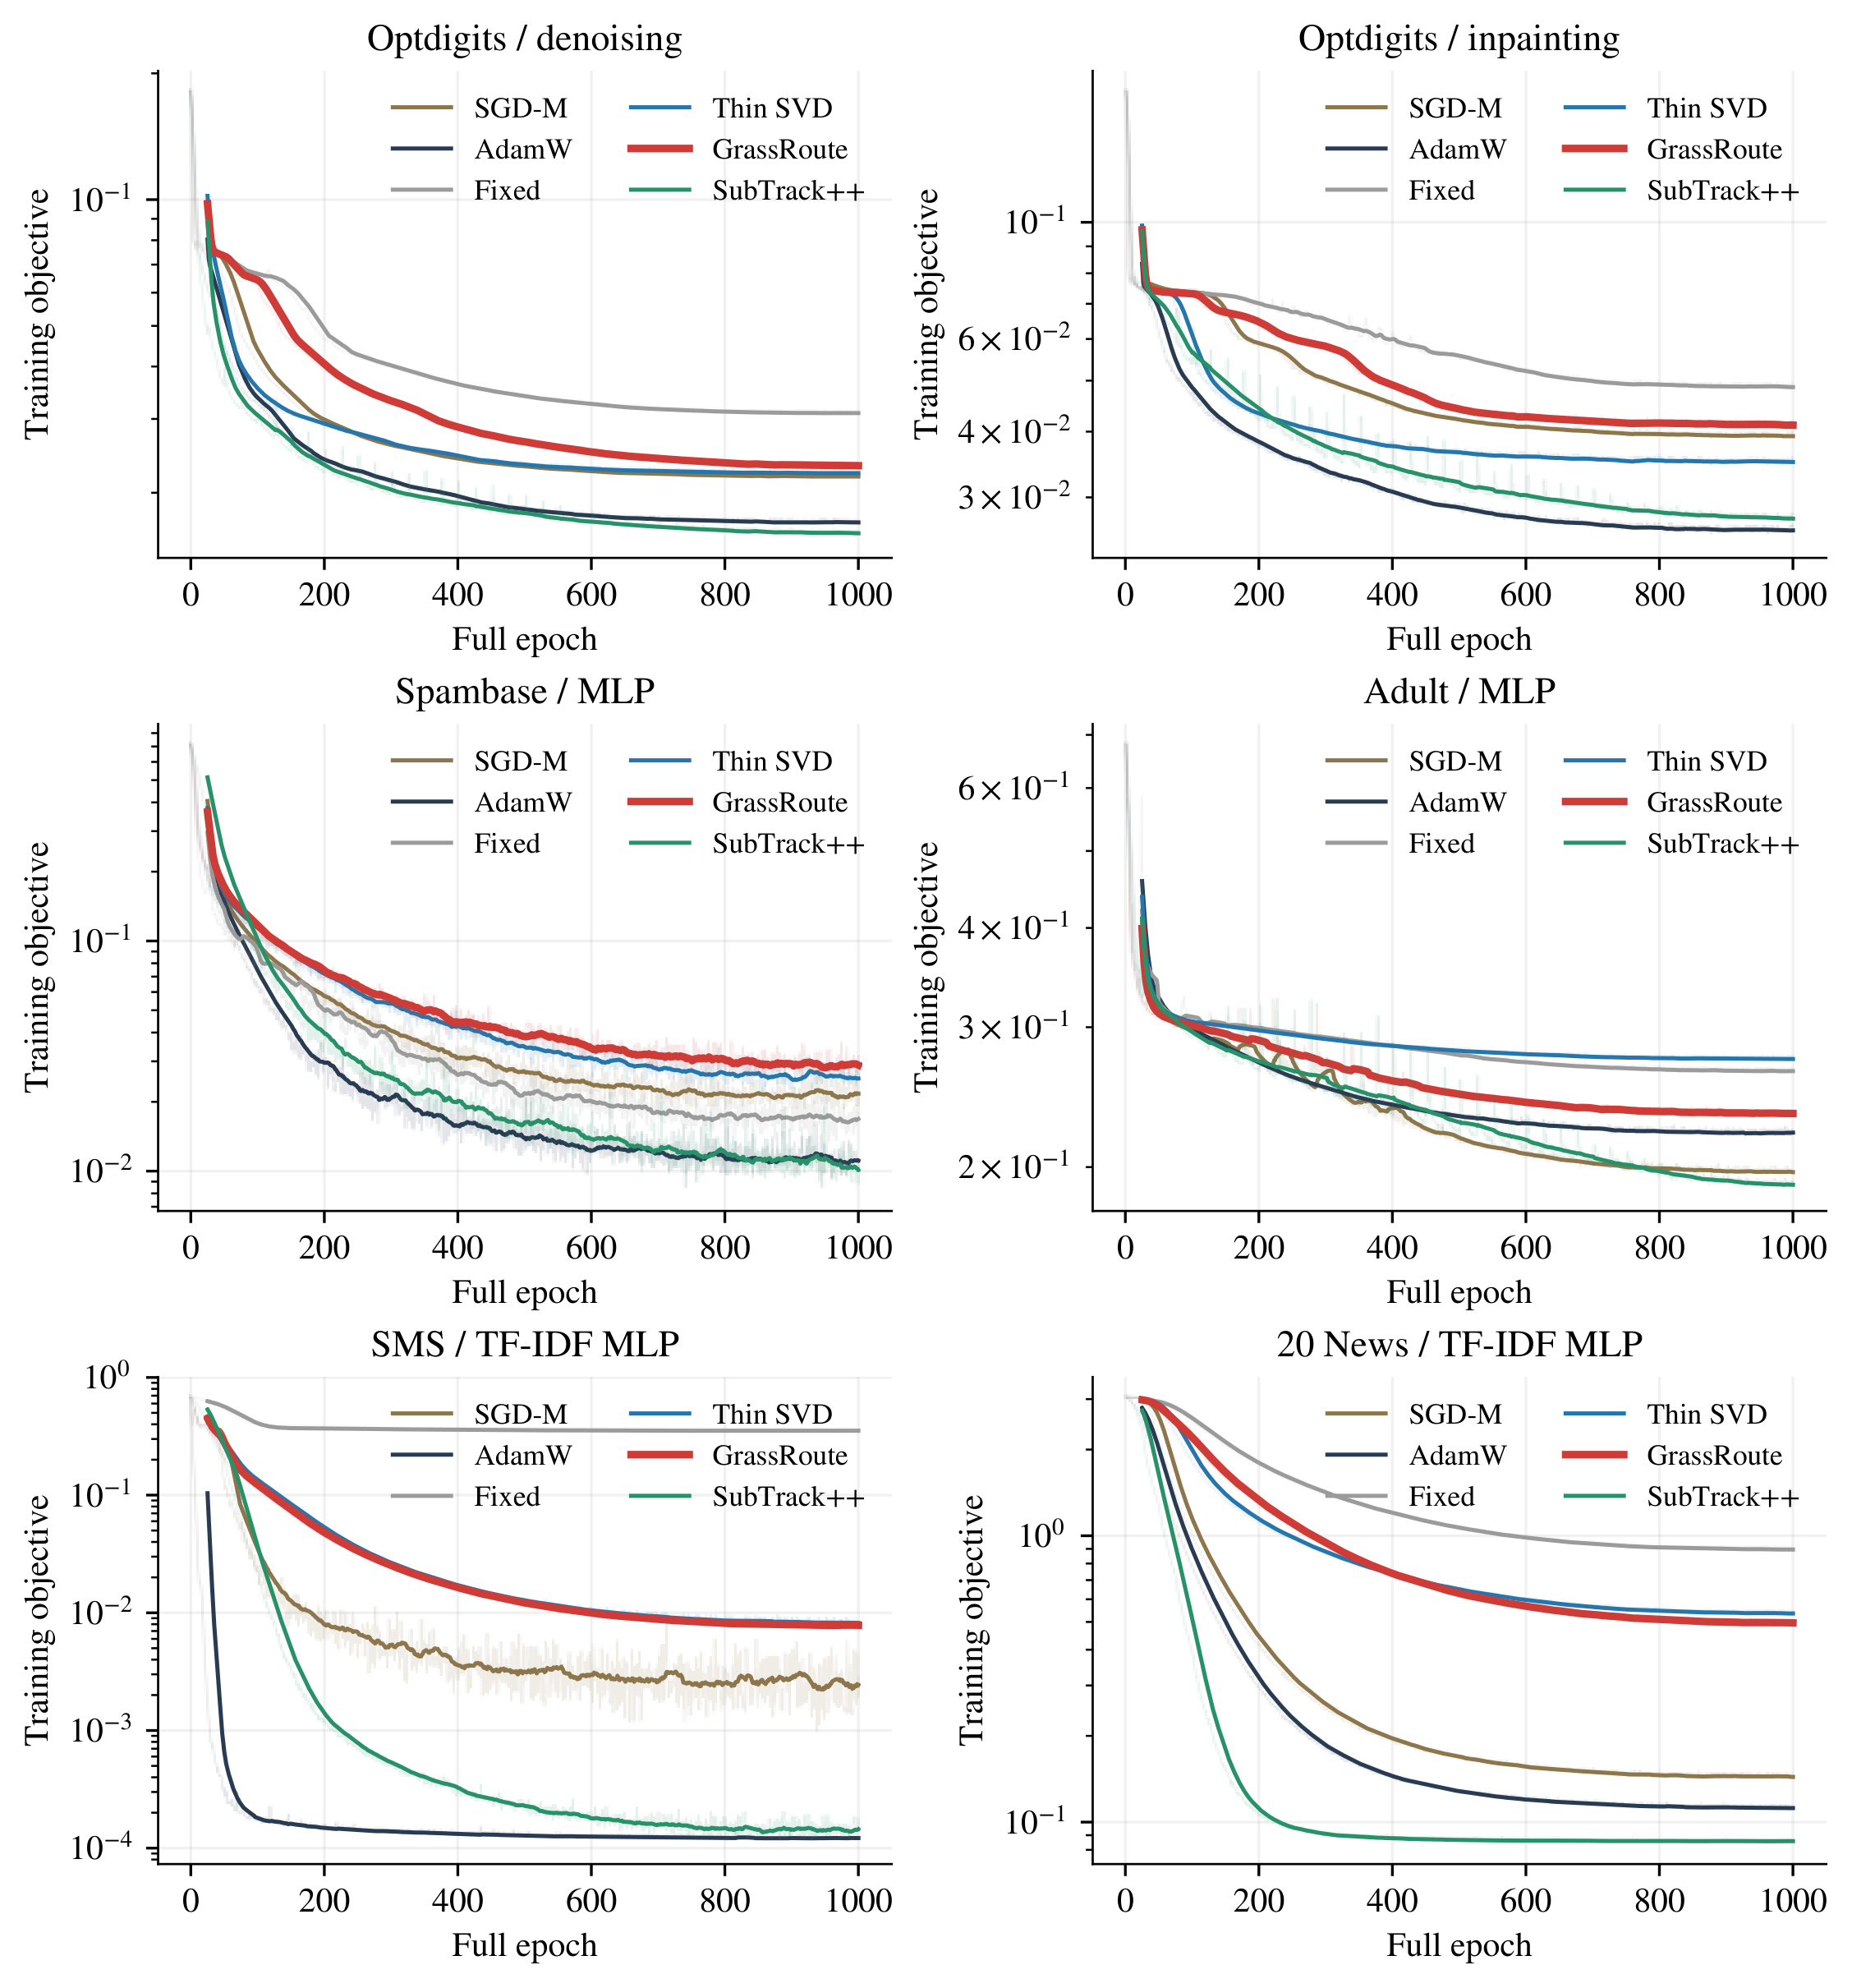
\includegraphics[width=\linewidth]{figures/fig_newtask_losses_all.png}
\caption{Complete new-task training-loss matrix, including every completed
formal optimizer run. Missing curves indicate unfinished or failed formal
training, never an omitted unfavorable endpoint. All full runs have 1000
epochs. Faint lines are raw objectives and solid lines are 25-epoch trailing
means. Task selection for the main-text illustration does not remove any
curve from this complete matrix.}
\label{fig:newtasks-all}
\end{figure}


\end{document}
